%% LyX 2.4.3 created this file.  For more info, see https://www.lyx.org/.
%% Do not edit unless you really know what you are doing.
\documentclass[journal,article,submit,pdftex,moreauthors]{Definitions/mdpi}
\usepackage[utf8]{inputenc}
\usepackage{color}
\usepackage{array}
\usepackage{float}
\usepackage{url}
\usepackage{varwidth}
\usepackage{amsmath}
\usepackage{graphicx}
\usepackage{rotfloat}

\makeatletter

%%%%%%%%%%%%%%%%%%%%%%%%%%%%%% LyX specific LaTeX commands.

\Title{The Echo Optimizer: A Novel Metaheuristic Inspired by Acoustic Reflection
Principles}

\TitleCitation{The Echo Optimizer: A Novel Metaheuristic Inspired by Acoustic Reflection
Principles}

\Author{Vasileios Charilogis$^{1}$, Ioannis G. Tsoulos$^{2,*}$ }

\AuthorNames{Vasileios Charilogis, Ioannis G. Tsoulos}

\AuthorCitation{Charilogis, V.; Tsoulos, I.G.}


\address{$^{1}$\quad{}Department of Informatics and Telecommunications,
University of Ioannina, 47150 Kostaki Artas, Greece; v.charilog@uoi.gr\\
$^{2}$\quad{}Department of Informatics and Telecommunications, University
of Ioannina, 47150 Kostaki Artas, Greece; itsoulos@uoi.gr}


\corres{Correspondence: itsoulos@uoi.gr}


\abstract{The Echo Optimizer Method is an innovative optimization technique
inspired by the natural behavior of sound echoes. It is based on generating
modified solutions (echoes) that combine directed reflection toward
the best-known solution and random noise that attenuates over time.
The method introduces two groundbreaking mechanisms to enhance performance:
an approximate evaluation system that avoids costly computations for
unpromising solutions, and an echo memory that stores and reuses past
evaluations. These mechanisms enable a significant reduction in computational
resources (up to 40--60\% fewer evaluations) while maintaining the
method's effectiveness. The Echo Optimizer excels in balancing exploration
of the solution space with exploitation of the best-known solutions,
demonstrating impressive performance in problems with numerous local
minima and high dimensionality. Experimental tests on standard optimization
problems have shown faster convergence and reduced result variability
compared to classical methods, making it a highly attractive choice
for various optimization challenges, particularly in cases where evaluating
the objective function is computationally expensive.}


\keyword{Optimization; Echo Optimizer; Evolutionary Algorithms; Global Optimization;
Adaptive Termination; Mutation Strategies; Metaheuristics;}

\newcommand*\LyXZeroWidthSpace{\hspace{0pt}}
\DeclareTextSymbolDefault{\textquotedbl}{T1}
%% Because html converters don't know tabularnewline
\providecommand{\tabularnewline}{\\}
%% Variable width box for table cells
\newenvironment{cellvarwidth}[1][t]
    {\begin{varwidth}[#1]{\linewidth}}
    {\@finalstrut\@arstrutbox\end{varwidth}}
\floatstyle{ruled}
\newfloat{algorithm}{tbp}{loa}
\providecommand{\algorithmname}{Algorithm}
\floatname{algorithm}{\protect\algorithmname}

%%%%%%%%%%%%%%%%%%%%%%%%%%%%%% User specified LaTeX commands.
\usepackage{rotating}

%  LaTeX support: latex@mdpi.com 
%  For support, please attach all files needed for compiling as well as the log file, and specify your operating system, LaTeX version, and LaTeX editor.

%=================================================================


% For posting an early version of this manuscript as a preprint, you may use "preprints" as the journal and change "submit" to "accept". The document class line would be, e.g., \documentclass[preprints,article,accept,moreauthors,pdftex]{mdpi}. This is especially recommended for submission to arXiv, where line numbers should be removed before posting. For preprints.org, the editorial staff will make this change immediately prior to posting.

%--------------------
% Class Options:
%--------------------
%----------
% journal
%----------
% Choose between the following MDPI journals:
% acoustics, actuators, addictions, admsci, adolescents, aerospace, agriculture, agriengineering, agronomy, ai, algorithms, allergies, alloys, analytica, animals, antibiotics, antibodies, antioxidants, applbiosci, appliedchem, appliedmath, applmech, applmicrobiol, applnano, applsci, aquacj, architecture, arts, asc, asi, astronomy, atmosphere, atoms, audiolres, automation, axioms, bacteria, batteries, bdcc, behavsci, beverages, biochem, bioengineering, biologics, biology, biomass, biomechanics, biomed, biomedicines, biomedinformatics, biomimetics, biomolecules, biophysica, biosensors, biotech, birds, bloods, blsf, brainsci, breath, buildings, businesses, cancers, carbon, cardiogenetics, catalysts, cells, ceramics, challenges, chemengineering, chemistry, chemosensors, chemproc, children, chips, cimb, civileng, cleantechnol, climate, clinpract, clockssleep, cmd, coasts, coatings, colloids, colorants, commodities, compounds, computation, computers, condensedmatter, conservation, constrmater, cosmetics, covid, crops, cryptography, crystals, csmf, ctn, curroncol, currophthalmol, cyber, dairy, data, dentistry, dermato, dermatopathology, designs, diabetology, diagnostics, dietetics, digital, disabilities, diseases, diversity, dna, drones, dynamics, earth, ebj, ecologies, econometrics, economies, education, ejihpe, electricity, electrochem, electronicmat, electronics, encyclopedia, endocrines, energies, eng, engproc, ent, entomology, entropy, environments, environsciproc, epidemiologia, epigenomes, est, fermentation, fibers, fintech, fire, fishes, fluids, foods, forecasting, forensicsci, forests, foundations, fractalfract, fuels, futureinternet, futureparasites, futurepharmacol, futurephys, futuretransp, galaxies, games, gases, gastroent, gastrointestdisord, gels, genealogy, genes, geographies, geohazards, geomatics, geosciences, geotechnics, geriatrics, hazardousmatters, healthcare, hearts, hemato, heritage, highthroughput, histories, horticulturae, humanities, humans, hydrobiology, hydrogen, hydrology, hygiene, idr, ijerph, ijfs, ijgi, ijms, ijns, ijtm, ijtpp, immuno, informatics, information, infrastructures, inorganics, insects, instruments, inventions, iot, j, jal, jcdd, jcm, jcp, jcs, jdb, jeta, jfb, jfmk, jimaging, jintelligence, jlpea, jmmp, jmp, jmse, jne, jnt, jof, joitmc, jor, journalmedia, jox, jpm, jrfm, jsan, jtaer, jzbg, kidney, kidneydial, knowledge, land, languages, laws, life, liquids, literature, livers, logics, logistics, lubricants, lymphatics, machines, macromol, magnetism, magnetochemistry, make, marinedrugs, materials, materproc, mathematics, mca, measurements, medicina, medicines, medsci, membranes, merits, metabolites, metals, meteorology, methane, metrology, micro, microarrays, microbiolres, micromachines, microorganisms, microplastics, minerals, mining, modelling, molbank, molecules, mps, msf, mti, muscles, nanoenergyadv, nanomanufacturing, nanomaterials, ncrna, network, neuroglia, neurolint, neurosci, nitrogen, notspecified, nri, nursrep, nutraceuticals, nutrients, obesities, oceans, ohbm, onco, oncopathology, optics, oral, organics, organoids, osteology, oxygen, parasites, parasitologia, particles, pathogens, pathophysiology, pediatrrep, pharmaceuticals, pharmaceutics, pharmacoepidemiology, pharmacy, philosophies, photochem, photonics, phycology, physchem, physics, physiologia, plants, plasma, pollutants, polymers, polysaccharides, poultry, powders, preprints, proceedings, processes, prosthesis, proteomes, psf, psych, psychiatryint, psychoactives, publications, quantumrep, quaternary, qubs, radiation, reactions, recycling, regeneration, religions, remotesensing, reports, reprodmed, resources, rheumato, risks, robotics, ruminants, safety, sci, scipharm, seeds, sensors, separations, sexes, signals, sinusitis, skins, smartcities, sna, societies, socsci, software, soilsystems, solar, solids, sports, standards, stats, stresses, surfaces, surgeries, suschem, sustainability, symmetry, synbio, systems, taxonomy, technologies, telecom, test, textiles, thalassrep, thermo, tomography, tourismhosp, toxics, toxins, transplantology, transportation, traumacare, traumas, tropicalmed, universe, urbansci, uro, vaccines, vehicles, venereology, vetsci, vibration, viruses, vision, waste, water, wem, wevj, wind, women, world, youth, zoonoticdis 

%---------
% article
%---------
% The default type of manuscript is "article", but can be replaced by: 
% abstract, addendum, article, book, bookreview, briefreport, casereport, comment, commentary, communication, conferenceproceedings, correction, conferencereport, entry, expressionofconcern, extendedabstract, datadescriptor, editorial, essay, erratum, hypothesis, interestingimage, obituary, opinion, projectreport, reply, retraction, review, perspective, protocol, shortnote, studyprotocol, systematicreview, supfile, technicalnote, viewpoint, guidelines, registeredreport, tutorial
% supfile = supplementary materials

%----------
% submit
%----------
% The class option "submit" will be changed to "accept" by the Editorial Office when the paper is accepted. This will only make changes to the frontpage (e.g., the logo of the journal will get visible), the headings, and the copyright information. Also, line numbering will be removed. Journal info and pagination for accepted papers will also be assigned by the Editorial Office.

%------------------
% moreauthors
%------------------
% If there is only one author the class option oneauthor should be used. Otherwise use the class option moreauthors.

%---------
% pdftex
%---------
% The option pdftex is for use with pdfLaTeX. If eps figures are used, remove the option pdftex and use LaTeX and dvi2pdf.

%=================================================================
% MDPI internal commands - do not modify
\firstpage{1} 
 
\setcounter{page}{\@firstpage} 

\pubvolume{1}
\issuenum{1}
\articlenumber{0}
\pubyear{2024}
\copyrightyear{2024}
%\externaleditor{Academic Editor: Firstname Lastname} % For journal Automation, please change Academic Editor to "Communicated by"
\datereceived{}
\daterevised{ } % Comment out if no revised date
\dateaccepted{}
\datepublished{}
%\datecorrected{} % Corrected papers include a "Corrected: XXX" date in the original paper.
%\dateretracted{} % Corrected papers include a "Retracted: XXX" date in the original paper.
\hreflink{https://doi.org/} % If needed use \linebreak
%\doinum{}
%------------------------------------------------------------------
% The following line should be uncommented if the LaTeX file is uploaded to arXiv.org
%\pdfoutput=1

%=================================================================
% Add packages and commands here. The following packages are loaded in our class file: fontenc, inputenc, calc, indentfirst, fancyhdr, graphicx, epstopdf, lastpage, ifthen, lineno, float, amsmath, setspace, enumitem, mathpazo, booktabs, titlesec, etoolbox, tabto, xcolor, soul, multirow, microtype, tikz, totcount, changepage, attrib, upgreek, cleveref, amsthm, hyphenat, natbib, hyperref, footmisc, url, geometry, newfloat, caption

%=================================================================
%% Please use the following mathematics environments: Theorem, Lemma, Corollary, Proposition, Characterization, Property, Problem, Example, ExamplesandDefinitions, Hypothesis, Remark, Definition, Notation, Assumption
%% For proofs, please use the proof environment (the amsthm package is loaded by the MDPI class).

%=================================================================
% The fields PACS, MSC, and JEL may be left empty or commented out if not applicable
%\PACS{J0101}
%\MSC{}
%\JEL{}

%%%%%%%%%%%%%%%%%%%%%%%%%%%%%%%%%%%%%%%%%%
% Only for the journal Diversity
%\LSID{\url{http://}}

%%%%%%%%%%%%%%%%%%%%%%%%%%%%%%%%%%%%%%%%%%
% Only for the journal Applied Sciences:
%\featuredapplication{Authors are encouraged to provide a concise description of the specific application or a potential application of the work. This section is not mandatory.}
%%%%%%%%%%%%%%%%%%%%%%%%%%%%%%%%%%%%%%%%%%

%%%%%%%%%%%%%%%%%%%%%%%%%%%%%%%%%%%%%%%%%%
% Only for the journal Data:
%\dataset{DOI number or link to the deposited data set in cases where the data set is published or set to be published separately. If the data set is submitted and will be published as a supplement to this paper in the journal Data, this field will be filled by the editors of the journal. In this case, please make sure to submit the data set as a supplement when entering your manuscript into our manuscript editorial system.}

%\datasetlicense{license under which the data set is made available (CC0, CC-BY, CC-BY-SA, CC-BY-NC, etc.)}

%%%%%%%%%%%%%%%%%%%%%%%%%%%%%%%%%%%%%%%%%%
% Only for the journal Toxins
%\keycontribution{The breakthroughs or highlights of the manuscript. Authors can write one or two sentences to describe the most important part of the paper.}

%%%%%%%%%%%%%%%%%%%%%%%%%%%%%%%%%%%%%%%%%%
% Only for the journal Encyclopedia
%\encyclopediadef{Instead of the abstract}
%\entrylink{The Link to this entry published on the encyclopedia platform.}
%%%%%%%%%%%%%%%%%%%%%%%%%%%%%%%%%%%%%%%%%%

%%%%%%%%%%%%%%%%%%%%%%%%%%%%%%%%%%%%%%%%%%
% Only for the journal Advances in Respiratory Medicine
%\addhighlights{yes}
%\renewcommand{\addhighlights}{%

%\noindent This is an obligatory section in “Advances in Respiratory Medicine”, whose goal is to increase the discoverability and readability of the article via search engines and other scholars. Highlights should not be a copy of the abstract, but a simple text allowing the reader to quickly and simplified find out what the article is about and what can be cited from it. Each of these parts should be devoted up to 2~bullet points.\vspace{3pt}\\
%\textbf{What are the main findings?}
% \begin{itemize}[labelsep=2.5mm,topsep=-3pt]
% \item First bullet.
% \item Second bullet.
% \end{itemize}\vspace{3pt}
%\textbf{What is the implication of the main finding?}
% \begin{itemize}[labelsep=2.5mm,topsep=-3pt]
% \item First bullet.
% \item Second bullet.
% \end{itemize}
%}
%%%%%%%%%%%%%%%%%%%%%%%%%%%%%%%%%%%%%%%%%%
% Added by lyx2lyx
\usepackage{array}

\makeatother

\begin{document}
\maketitle

\section{Introduction}

Global optimization deals with finding the absolute lowest point (global
minimum) of a continuous objective function $f(x)$ defined over a
bounded, n-dimensional search space $S$. Mathematically, the goal
is to identify the point $x^{*}$ in $S$ where $f(x)$ attains its
smallest possible value:

\begin{equation}
x^{*}=\mbox{arg}\min_{x\in S}f(x).
\end{equation}
where:
\begin{itemize}
\item $f(x)$ is the objective function to minimize (e.g., cost, error,
or energy).
\item $S$ is a compact (closed and bounded) subset of $R^{n}$, often defined
as an n-dimensional hyperrectangle:
\end{itemize}
\textbf{
\[
S=\left[a_{1},b_{1}\right]\otimes\left[a_{2},b_{2}\right]\otimes\ldots\left[a_{n},b_{n}\right]
\]
}

Here, $a_{i}$ and $b_{i}$ are the lower and upper bounds for each
variable$x_{i}$, confining the search to a specific region.

Optimization constitutes a central field of computational mathematics
with applications to multifaceted scientific and industrial problems.
Optimization methods are classified into broad categories according
to their underlying strategies and the properties of the problems
they address. Among the most well-known techniques are classical gradient
methods such as steepest descent \citep{Tapkin} and Newton's method
\citep{Cawade}, stochastic methods like Monte Carlo \citep{Bonate}
algorithms and simulated annealing \citep{Eglese,Siarry} population-based
methods including genetic algorithms \citep{Sohail} and differential
evolution \citep{Deng,Pant,Charilogis,Charilogis2}, convex optimization
methods such as the ellipsoid method \citep{Vishnoi,Vishnoi-1} and
cutting-plane method \citep{Pi=0000F3ro}, simplex-based methods like
the Nelder-Mead method \citep{Nelder}, response surface methods including
krigin \citep{Jones}, trust-region methods like Bayesian optimization
\citep{Snoek,Mockus}, conjugate gradient methods such as Fletcher-Reeves
\citep{Fletcher} and Polak-Ribière \citep{Polak,Nocedal}, constrained
optimization methods including penalty function methods and interior-point
methods, decomposition approaches like Benders decomposition \citep{Benders,Geoffrion}
and Dantzig-Wolfe decomposition \citep{Dantzig}, space-partitioning
methods such as DIRECT \citep{Jones-1} and branch-and-bound \citep{Land,Lemarechal},
neural network-based methods including reinforcement learning algorithms,
socially-inspired methods like particle swarm optimization \citep{Shami,Gad}
and ant colony optimization \citep{Dorigo}, physics-inspired methods
including crystal structure optimization \citep{Rappoport} and gravitational
search algorithms \citep{Rashedi}, hybrid methods such as neuro-fuzzy
algorithms \citep{Jang}, and biologically-inspired methods like photosynthesis
algorithms \citep{Zhang-1} and DNA-based computing \citep{Adleman}.

Within this context, the Echo Optimizer method (EO) introduces a novel
approach based on the physical analogy of sound echoes. The core concept
involves generating modified solutions that simulate sound reflection,
with systematic adjustment of exploration intensity through a decay
factor. This technique combines elements from population-based methods
and stochastic techniques, offering a flexible mechanism for addressing
diverse optimization problems. The method's ability to balance solution
space exploration with exploitation of known optimal solutions makes
it particularly effective for high-dimensional problems and non-convex
functions.

The presentation of the method will focus on its theoretical foundations,
algorithmic design, and experimental performance compared to other
contemporary techniques. Furthermore, we will analyze its application
potential to real-world problems, along with the challenges arising
from its use in complex systems. This work aims to highlight the method's
distinctive properties that make it a valuable addition to the toolkit
of modern optimization techniques.

The rest of the paper is organized as follows:

The introduction provides the background and motivation for the study.
The Echo Optimizer method is presented in Section \ref{sec:echoMethod},
detailing the core algorithm and its components. Subsection \ref{subsec:approEval}
introduces the technique of approximate evaluations, while Subsection
\ref{subsec:memoryEcho} describes the technique of echo memory. Followed
by subsection \ref{subsec:overalAlgorithm} where the complete algorithm
is described. The experimental setup and benchmark results are discussed
in Section \ref{sec:Results}, which includes an overview of the benchmark
functions in Subsection \ref{subsec:benchmarkFunctions} and the experimental
results in Subsection \ref{subsec:experimentalResults}. Finally,
the conclusions are presented in Section \ref{sec:Conclusions}, summarizing
the key findings and implications of the study.

\section{The Echo Optimizer method \label{sec:echoMethod}}

The EO algorithm is an evolutionary method inspired by the natural
behavior of sound echoes, combining mathematical optimization strategies
with physical analogies. Its core principle lies in generating solutions
(called \textquotedbl echoes\textquotedbl ) through a directed reflection
of current solutions towards the best-known solution, coupled with
the addition of random noise that attenuates over time. The initial
population of solutions is generated randomly within the bounds of
the search space, and each solution is evaluated based on an objective
function. During each iteration, solutions are updated using a combination
of directed reflection, which pulls them closer to the best-known
solution, and random noise, which allows exploration of new regions
in the solution space. The noise diminishes as the algorithm progresses,
enabling a transition from exploration to exploitation. This mechanism
ensures the algorithm’s ability to balance the discovery of new potential
solutions with the refinement of promising ones, making it effective
for tackling high-dimensional problems and complex landscapes with
multiple local minima.

The basic EO algorithm generates new solutions, called echoes, based
on a combination of directed reflection and random noise.

For each dimension $d$ of the solution $x_{i}$\LyXZeroWidthSpace ,
the updated value $echo_{d}$ is computed as:

\begin{equation}
echo_{d}=x_{i,d}+coef\cdot(x_{best,d}-x_{i,d})+noise_{d}
\end{equation}

Where:
\begin{itemize}
\item $coef\cdot(x_{best,d}-x_{i,d})$: A directed reflection term that
moves the solution toward the best-known solution $x_{best}$.
\item $coef$: Reflection factor
\item $noise_{d}=random[-1,1]\cdot(1-currentDelay)$: A random noise term
that attenuates as $currentDelay$ decreases over iterations.
\item $currentDelay=initDelay-(initDelay-finalDelay)\cdot(\frac{iter}{iter_{max}})$:
A decay factor that adjusts over the course of $iter_{max}$ iterations.
\end{itemize}

\subsection{The echo memory technique \label{subsec:memoryEcho}}

The memory technique introduces a unique mechanism to the EO algorithm
by enabling the storage and reuse of information from previously evaluated
solutions, significantly reducing computational overhead. Specifically,
each evaluated solution is stored in an echo memory along with its
corresponding objective function value. When a new solution is generated,
the algorithm checks if a similar solution exists in memory, using
a predefined tolerance level to determine similarity. If a match is
found, the stored value is retrieved instead of recalculating the
objective function. This feature is particularly beneficial in problems
where evaluating solutions is computationally expensive. Moreover,
the memory is dynamically updated with new, improved solutions, ensuring
the algorithm’s adaptability to evolving optimization scenarios. This
mechanism enhances the algorithm's efficiency by focusing computational
resources on exploring truly novel areas of the search space, rather
than redundantly evaluating similar solutions.

In the memory-enhanced EO configuration, the algorithm stores previously
evaluated solutions and their corresponding fitness values to avoid
redundant computations. When a new solution echo is generated, the
algorithm checks if a similar solution exists in the memory within
a predefined tolerance ($e$: small number e.g. 0.5):

\begin{equation}
|echo_{d}-memory_{j,d}|<e
\end{equation}

If a match is found:
\begin{itemize}
\item Retrieve $memoryFitness_{j}$.
\item If $memoryFitness_{j}$\textless{} $f_{i}$, update the current solution
and its fitness:
\begin{itemize}
\item $x_{i}=echo$
\item $f_{i}=memoryFitness_{j}$
\end{itemize}
\end{itemize}
Similarity in the EO method is determined exclusively by the Euclidean
distance between the coordinates of the candidate solution and those
stored in memory. Similarity is evaluated by comparing the differences
in the coordinate values for each dimension. If the absolute difference
between the respective values is smaller than the predefined tolerance,
the solution is considered similar to one already stored in memory.
The calculation is based on the Equation 3, where the result is compared
against the tolerance value $e$ (Table \ref{tab:settings}). The
objective function values are not used in the similarity determination
process. The evaluation relies solely on geometric proximity, specifically
the position of the solutions within the search space.

\subsection{The approximate evaluations technique \label{subsec:approEval}}

The approximation technique allows the algorithm to estimate the quality
of solutions quickly and efficiently, avoiding unnecessary computations
for solutions that are unlikely to provide improvements. When a new
solution is generated, instead of immediately evaluating it using
the objective function, the algorithm applies an approximation function
to predict its quality based on its proximity to the best-known solution.
If the approximation exceeds a predefined threshold, the solution
is rejected without further processing. This selective evaluation
process accelerates convergence by focusing on promising solutions
and reducing the number of expensive objective function calculations.
The approximation technique thus improves the algorithm's speed without
sacrificing accuracy or its ability to explore the solution space,
making it particularly efficient in scenarios where objective function
evaluations are resource-intensive.

In the configuration with approximate evaluations, the algorithm uses
a heuristic to estimate the quality of a solution before computing
the objective function. The approximate fitness is calculated as:

\begin{equation}
approxFitness=\left(\sum_{d=1}^{n}(echo_{d}-x_{best,d})^{2}\right)\cdot currentDelay
\end{equation}

If: $approxFitness>approxThreshold\cdot f_{i}$: 

then the solution is rejected without evaluating the objective function,
and the algorithm proceeds to the next individual.

\medskip{}

The memory and approximation techniques in the EO differ from similar
approaches such as Long Term Memory Assistance for Evolutionary Algorithms
(LTMA) \citep{Crepinsek} and Surrogate Modelling \citep{Loper},
both in philosophy and implementation. In the case of memory, EO utilizes
a dynamic storage structure that contains previously evaluated solutions
and their fitness values. This mechanism avoids redundant computations
by comparing new solutions with those already stored in memory and
using the stored fitness value if the new solution is sufficiently
similar. In contrast, LTMA maintains historical data from previous
generations of evolutionary algorithms and focuses on strategically
guiding the optimization process based on long-term trends and changes
in the population of solutions. EO’s memory mechanism is more localized
and aimed at reducing computational costs, while LTMA operates on
a broader scale, emphasizing exploration guidance. Regarding approximation
techniques, EO relies on heuristic estimates to discard unpromising
solutions before the objective function is evaluated. These estimates
are based on the distance of the new solution from the best-known
solution and a decay factor that adjusts over the iterations. On the
other hand, Surrogate Modelling creates accurate mathematical or statistical
models, such as Gaussian Processes, to approximate the objective function.
These models require training on previously evaluated data points
and are used to select the most promising solutions. EO employs a
lighter approach suitable for rapid execution, whereas Surrogate Modeling
offers higher accuracy but comes with greater computational cost.
Overall, EO emphasizes simplicity and reduced computational overhead,
while LTMA and Surrogate Modelling pursue strategic guidance and increased
accuracy, respectively, often at the expense of higher resource and
time requirements.

\subsection{The overall algorithm\label{subsec:overalAlgorithm}}

The overall algorithm of the method follows:
\begin{algorithm}[H]
{\footnotesize Algorithm: Echo Optimization with Approximate Evaluations
and Memory}{\footnotesize\par}

{\footnotesize Input:}{\footnotesize\par}

{\footnotesize - $NP$: Population size}{\footnotesize\par}

{\footnotesize - $initDelay\in[0,1]$: Initial delay factor}{\footnotesize\par}

{\footnotesize - $finalDelay\in[0,1]$: Final delay factor}{\footnotesize\par}

{\footnotesize - $reflectionFactor\in[0,1]$: Reflection coefficient}{\footnotesize\par}

{\footnotesize - $iter_{max}$: Maximum iterations}{\footnotesize\par}

{\footnotesize - $approxThreshold$: Approximation threshold (e.g.,
0.2 - 20\%)}{\footnotesize\par}

{\footnotesize - $maxMemorySize$: Memory capacity}{\footnotesize\par}

{\footnotesize - $technique\in$\{ECHO, ECHO+APP, ECHO+MEM, ECHO+APP+MEM\}:
Variant selection}{\footnotesize\par}

{\footnotesize - $searchSpace$: Feasible solution bounds}{\footnotesize\par}

{\footnotesize Output:}{\footnotesize\par}

{\footnotesize - $x_{best}$: Optimal solution found, $f_{best}$:
Corresponding fitness value}{\footnotesize\par}

{\footnotesize Initialization:}{\footnotesize\par}

{\footnotesize 01: Initialize population $X=\{x_{i}|x_{i}~U(searchSpace),i=1,...,NP$\}}{\footnotesize\par}

{\footnotesize 02: Evaluate initial fitness $F=\{f=f(x_{i})|i=1,...,NP\}$}{\footnotesize\par}

{\footnotesize 03: Set ($x_{best}$, $f_{best}$) = $argmin_{(x_{i},f_{i})}f_{i}$}{\footnotesize\par}

{\footnotesize 04: Initialize empty memory: $M=\varnothing$, $F_{M}=\varnothing$}{\footnotesize\par}

{\footnotesize Main Optimization Loop:}{\footnotesize\par}

{\footnotesize 05: for iter = 1 to $iter_{max}$ do}{\footnotesize\par}

{\footnotesize 06: \hspace{0.5cm}$currentDelay=initDelay-(initDelay-finalDelay)\cdot(\frac{iter}{iter_{max}})$}{\footnotesize\par}

{\footnotesize 07: \hspace{0.5cm}for each individual $x_{i}$ in $X$
do}{\footnotesize\par}

{\footnotesize 08: \hspace{0.5cm}\hspace{0.5cm}// Echo vector generation}{\footnotesize\par}

{\footnotesize 09: \hspace{0.5cm}\hspace{0.5cm}for d = 1 to dim do}{\footnotesize\par}

{\footnotesize 10: \hspace{0.5cm}\hspace{0.5cm}\hspace{0.5cm}$echo_{d}=x_{i,d}+coef\cdot(x_{best,d}-x_{i,d})+U(-1,1)\cdot(1-currentDelay)$}{\footnotesize\par}

{\footnotesize 11: \hspace{0.5cm}\hspace{0.5cm}\hspace{0.5cm}$echo_{d}=clamp(echo_{d},searchSpace.lower_{d},searchSpace.upper_{d})$}{\footnotesize\par}

{\footnotesize 12: \hspace{0.5cm}\hspace{0.5cm}end for}{\footnotesize\par}

{\footnotesize 13: \hspace{0.5cm}\hspace{0.5cm}// Approximation evaluation
(Optional)}{\footnotesize\par}

{\footnotesize 14: \hspace{0.5cm}\hspace{0.5cm}if $technique$ =
\textquotedbl ECHO+APP\textquotedbl{} then}{\footnotesize\par}

{\footnotesize 15: \hspace{0.5cm}\hspace{0.5cm}\hspace{0.5cm}$approxFitness=\left(\sum_{d=1}^{n}(echo_{d}-x_{best,d})^{2}\right)\cdot currentDelay$}{\footnotesize\par}

{\footnotesize 16: \hspace{0.5cm}\hspace{0.5cm}\hspace{0.5cm}if
$approxFitness>approxThreshold\cdot f_{i}$ then}{\footnotesize\par}

{\footnotesize 17: \hspace{0.5cm}\hspace{0.5cm}\hspace{0.5cm}\hspace{0.5cm}continue
to next individual}{\footnotesize\par}

{\footnotesize 18: \hspace{0.5cm}\hspace{0.5cm}\hspace{0.5cm}end
if}{\footnotesize\par}

{\footnotesize 19: \hspace{0.5cm}\hspace{0.5cm}end if}{\footnotesize\par}

{\footnotesize 20: \hspace{0.5cm}\hspace{0.5cm}// Memory lookup (Optional)}{\footnotesize\par}

{\footnotesize 21: \hspace{0.5cm}\hspace{0.5cm}if $technique$ =
\textquotedbl ECHO+MEM\textquotedbl{} then}{\footnotesize\par}

{\footnotesize 22: \hspace{0.5cm}\hspace{0.5cm}\hspace{0.5cm}if
$\exists j:||echo-M_{j}||<\varepsilon$ then}{\footnotesize\par}

{\footnotesize 23: \hspace{0.5cm}\hspace{0.5cm}\hspace{0.5cm}\hspace{0.5cm}if
$F_{M_{j}}<f_{i}$ then}{\footnotesize\par}

{\footnotesize 24: \hspace{0.5cm}\hspace{0.5cm}\hspace{0.5cm}\hspace{0.5cm}\hspace{0.5cm}$x_{i}\leftarrow echo$}{\footnotesize\par}

{\footnotesize 25: \hspace{0.5cm}\hspace{0.5cm}\hspace{0.5cm}\hspace{0.5cm}\hspace{0.5cm}$f_{i}\leftarrow F_{M_{j}}$}{\footnotesize\par}

{\footnotesize 26: \hspace{0.5cm}\hspace{0.5cm}\hspace{0.5cm}\hspace{0.5cm}\hspace{0.5cm}UpdateBest($x_{i}$,$f_{i}$)}{\footnotesize\par}

{\footnotesize 27: \hspace{0.5cm}\hspace{0.5cm}\hspace{0.5cm}\hspace{0.5cm}end
if}{\footnotesize\par}

{\footnotesize 28: \hspace{0.5cm}\hspace{0.5cm}\hspace{0.5cm}\hspace{0.5cm}continue
to next individual}{\footnotesize\par}

{\footnotesize 29: \hspace{0.5cm}\hspace{0.5cm}\hspace{0.5cm}end
if}{\footnotesize\par}

{\footnotesize 30: \hspace{0.5cm}\hspace{0.5cm}end if}{\footnotesize\par}

{\footnotesize 31: \hspace{0.5cm}\hspace{0.5cm}// Full evaluation}{\footnotesize\par}

{\footnotesize 32: \hspace{0.5cm}\hspace{0.5cm}$f_{echo}=f(echo)$}{\footnotesize\par}

{\footnotesize 33: \hspace{0.5cm}\hspace{0.5cm}if $f_{echo}\le f_{i}$
then}{\footnotesize\par}

{\footnotesize 34: \hspace{0.5cm}\hspace{0.5cm}\hspace{0.5cm}$x_{i}\leftarrow echo$}{\footnotesize\par}

{\footnotesize 35: \hspace{0.5cm}\hspace{0.5cm}\hspace{0.5cm}$f_{i}\leftarrow f_{echo}$}{\footnotesize\par}

{\footnotesize 36: \hspace{0.5cm}\hspace{0.5cm}\hspace{0.5cm}UpdateBest($x_{i}$,$f_{i}$) }{\footnotesize\par}

{\footnotesize 37: \hspace{0.5cm}\hspace{0.5cm}\hspace{0.5cm}//
Update memory (if applicable)}{\footnotesize\par}

{\footnotesize 38: \hspace{0.5cm}\hspace{0.5cm}\hspace{0.5cm}if
$technique$ = \textquotedbl memory\textquotedbl{} and $|M|<maxMemorySize$
then}{\footnotesize\par}

{\footnotesize 39: \hspace{0.5cm}\hspace{0.5cm}\hspace{0.5cm}\hspace{0.5cm}$M\leftarrow M\cup\{echo\}$}{\footnotesize\par}

{\footnotesize 40: \hspace{0.5cm}\hspace{0.5cm}\hspace{0.5cm}\hspace{0.5cm}$F_{M}\leftarrow F_{M}\cup\{f_{echo}\}$}{\footnotesize\par}

{\footnotesize 41: \hspace{0.5cm}\hspace{0.5cm}\hspace{0.5cm}end
if}{\footnotesize\par}

{\footnotesize 42: \hspace{0.5cm}\hspace{0.5cm}end if}{\footnotesize\par}

{\footnotesize 43: \hspace{0.5cm}end for}{\footnotesize\par}

{\footnotesize 44: \hspace{0.5cm}// Local search phase (Optional)\citep{Lam}}{\footnotesize\par}

{\footnotesize 45: \hspace{0.5cm}for each individual $x_{i}$ in $X$
do}{\footnotesize\par}

{\footnotesize 46: \hspace{0.5cm}\hspace{0.5cm}if $U(0,1)<localSearchRate$
then}{\footnotesize\par}

{\footnotesize 47: \hspace{0.5cm}\hspace{0.5cm}\hspace{0.5cm}$x_{refined},f_{refined}=localSearch(x_{i})$}{\footnotesize\par}

{\footnotesize 48: \hspace{0.5cm}\hspace{0.5cm}\hspace{0.5cm}if
$f_{refined}<f_{i}$ then}{\footnotesize\par}

{\footnotesize 59: \hspace{0.5cm}\hspace{0.5cm}\hspace{0.5cm}\hspace{0.5cm}$x_{i}\leftarrow x_{refined}$}{\footnotesize\par}

{\footnotesize 60: \hspace{0.5cm}\hspace{0.5cm}\hspace{0.5cm}\hspace{0.5cm}$f_{i}\leftarrow f_{refined}$}{\footnotesize\par}

{\footnotesize 61: \hspace{0.5cm}\hspace{0.5cm}\hspace{0.5cm}\hspace{0.5cm}UpdateBest($x_{i}$,$f_{i}$)}{\footnotesize\par}

{\footnotesize 62: \hspace{0.5cm}\hspace{0.5cm}\hspace{0.5cm}end
if}{\footnotesize\par}

{\footnotesize 63: \hspace{0.5cm}\hspace{0.5cm}end if}{\footnotesize\par}

{\footnotesize 64: \hspace{0.5cm}end for}{\footnotesize\par}

{\footnotesize 65: \hspace{0.5cm}if termination criteria $SR$ is
meet then end for\ref{tab:settings}}{\footnotesize\par}

{\footnotesize 66: end for}{\footnotesize\par}

{\footnotesize 67: return ($x_{best}$, $f_{best}$)}{\footnotesize\par}

\caption{Pseudocode of EO\label{alg:pseudocode}}
\end{algorithm}

The EO algorithm (Algorithm \ref{alg:pseudocode}) begins by initializing
its parameters, which include the population size $NP$, the initial
delay factor $initDelay$, the final delay factor $finalDelay$, the
reflection factor $coef$, the maximum number of iterations $iter_{max}$
, the approximation threshold $approxThreshold$, and the maximum
memory size $maxMemorySize$. A random population of solutions $x_{i}$
is generated within the predefined bounds of the search space, where
$i$ ranges from 1 to $NP$. Each solution in the population is evaluated
using the objective function to compute its fitness $f_{i}$. The
best solution, referred to as $x_{best},$ and its fitness $f_{best}$
are identified. An echo memory, echoMemory, is initialized as an empty
structure, along with its corresponding memory fitness values.

The optimization process enters the main loop, which runs for a maximum
of $iter_{max}$ iterations. At each iteration, the delay factor $currentDecay$
is computed as a linear interpolation between $initDelay$ and $finalDelay$,
depending on the current iteration $iter$ relative to $iter_{max}$.
For each solution $x_{i}$ in the population, a new solution (echo)
is generated dimension by dimension. The new value for each dimension
$echo_{d}$ is calculated by adding three components: the reflection
term, which directs the solution toward $x_{best,d}$, the noise term,
which introduces randomness and decreases as $currentDecay$ reduces
over time, and the original value of the dimension. Boundary correction
is applied to ensure the new solution remains within valid limits.

After generating the echo, optional techniques may be applied to enhance
computational efficiency. If the approximation technique is enabled,
an approximate fitness $approxFitness$ is calculated based on the
proximity of the echo to $x_{best}$. If $approxFitness$ exceeds
$approxThreshold\cdot f_{i}$ , the echo is discarded without further
evaluation, and the algorithm moves to the next solution. If the memory
technique is enabled, the algorithm checks whether the echo exists
in the echo memory within a tolerance. If a match is found, the stored
fitness value is used. If the stored fitness is better than the current
$f_{i}$ , $x_{i}$ and $f_{i}$ are updated accordingly. For echoes
that pass these checks or if the optional techniques are not applied,
the fitness of the echo $echoFitness$ is calculated by evaluating
the objective function. If $echoFitness$ is better than $f_{i}$
, the echo replaces the current solution $x_{i}$, and $f_{i}$ is
updated. If the echo is the best solution found so far, $x_{best}$
and $f_{best}$ are updated.

An optional local search phase may follow, where individual solutions
are refined with a certain probability. If the refined fitness improves
upon the current fitness, the solution and its fitness are updated.
The algorithm continues to iterate until $iter_{max}$ is reached
or a termination condition is met, at which point the best solution
$x_{best}$ is returned as the result of the optimization process.

\subsection{Parameters Sensitivity}

The reflection factor ($coef$), which regulates the attraction toward
the current best solution, directly affects the algorithm’s ability
to escape local minima. Values around 0.5 generally work well across
various problems, but for functions with steep gradients or many small
local minima, fine-tuning may be necessary. In contrast, the parameters
that control the linear decay exhibit greater stability, with default
values providing a balanced transition from exploration to exploitation
without causing major disruptions.

The approximation threshold ($approxThreshold$) determines the tendency
to reject candidate solutions and directly influences convergence
speed. Values near 0.2 provide an acceptable balance between accuracy
and speed. However, in problems with wide basins of attraction, it
can be increased up to 0.3 to accelerate the process, whereas in problems
with sharp ridges, it may be reduced to 0.1 to avoid mistakenly discarding
valid solutions. The local search rate may also require attention,
especially in problems with numerous local minima, as higher values
tend to improve reliability at the cost of increased computational
overhead.

For practical applications, it is recommended to begin with the default
parameter values, followed by gradual adjustments depending on the
problem type. Avoiding extreme values in sensitive parameters is important,
as values outside reasonable bounds can significantly degrade performance.
Empirical testing on representative problems remains the most reliable
strategy for parameter tuning, while the development of automatic
parameter control mechanisms would be a valuable extension in future
versions of the algorithm.

The memory tolerance parameter ($e$) is particularly sensitive and
directly affects the efficiency of the memory mechanism. The default
value of e = 0.5 works well for many problems, typically corresponding
to 5--10\% of the variable range in standard optimization benchmarks.
However, the optimal value depends on the characteristics of the objective
function. Small values (e \textless{} 0.2) greatly increase the number
of stored solutions, improving accuracy but also leading to excessive
memory usage, increased computational cost during similarity checks,
and a risk of overfitting to local variations. On the other hand,
large values (e \textgreater{} 1.0) reduce the effectiveness of memory
by allowing false associations between dissimilar solutions, lowering
reuse rates, and leading to redundant objective function evaluations.
For functions with steep slopes or narrow valleys (e.g., ROSENBROCK),
lower values (e = 0.2--0.4) are recommended to ensure accuracy. For
functions with wide attraction basins (e.g., SPHERE), higher values
(e = 0.6--0.8) improve reuse efficiency. In noisy functions, setting
e \ensuremath{\le} 0.3 helps avoid contamination of the memory with
unstable solutions. The interaction between e and the memory size
(maxMemorySize) is also critical. When memory is limited, a slightly
increased e improves coverage without overloading the system, while
in cases with large memory availability, a smaller e allows more precise
mapping of the search space. There is no universally optimal value;
selection must rely on experimental evaluation across representative
subproblems.

\section{Experimental setup and benchmark results \label{sec:Results}}

This section first introduces the benchmark functions selected for
experimental evaluation, followed by a comprehensive analysis of the
conducted experiments. The study systematically examines the various
parameters of the ECHO+APP+MEM algorithm to assess its reliability
and effectiveness in different optimization scenarios. The complete
parameter configurations used throughout these experiments are documented
in Table \ref{tab:settings}.

\begin{table}[H]
\caption{Parameters and settings \label{tab:settings}}

\centering{}{\footnotesize{}%
\begin{tabular}{|c|c|c|}
\hline 
{\footnotesize PARAMETER} & {\footnotesize VALUE} & {\footnotesize EXPLANATION}\tabularnewline
\hline 
\hline 
{\footnotesize$NP$} & {\footnotesize 200, 50, $4+\left\lfloor 3\cdot\log(\text{dimension})\right\rfloor $} & {\footnotesize Population}\tabularnewline
\hline 
{\footnotesize$iter_{max}$} & {\footnotesize 200} & {\footnotesize Maximum number of iterations for all methods}\tabularnewline
\hline 
{\footnotesize$initialDelay$} & {\footnotesize 0.9}$^{*}$  & {\footnotesize Initial echo delay factor for EO}\tabularnewline
\hline 
{\footnotesize$finalDelay$} & {\footnotesize 0.1}$^{*}$ & {\footnotesize Final echo delay factor for EO}\tabularnewline
\hline 
{\footnotesize$coef$} & {\footnotesize 0.5}$^{*}$ & {\footnotesize Reflection factor towards best solution for EO}\tabularnewline
\hline 
{\footnotesize$approxThreshold$} & {\footnotesize 0.2 (20\%)}$^{*}$ & {\footnotesize Approximate threshold for EO}\tabularnewline
\hline 
{\footnotesize$e$} & {\footnotesize 0.5$^{**}$} & {\footnotesize Echo memory tolerance for EO}\tabularnewline
\hline 
{\footnotesize$SR$} & {\footnotesize$\delta_{sim}^{(iter)}=\left|f_{sim,min}^{(iter)}-f_{sim,min}^{(iter-1)}\right|$
\citep{Gianni,Charilogis-1,Lagaris}} & {\footnotesize Stopping rule for all methods}\tabularnewline
\hline 
{\footnotesize$N_{s}$} & {\footnotesize 12} & {\footnotesize Similarity $count_{max}$ for stopping rule}\tabularnewline
\hline 
{\footnotesize$LS$} & {\footnotesize 0.02 (2\%), Tables: \ref{tab:echo}, \ref{tab:balance},
\ref{tab:callsLow200}} & {\footnotesize Local search rate}\tabularnewline
\hline 
{\footnotesize$T_{s}$} & {\footnotesize Tourament size 8 \citep{Goldberg}} & {\footnotesize Selection of GA}\tabularnewline
\hline 
{\footnotesize$C_{rate}$} & {\footnotesize double, 0.1 (10\%) (classic values) } & {\footnotesize Crossover for GA}\tabularnewline
\hline 
{\footnotesize$M_{rate}$} & {\footnotesize double, 0,05 (5\%) (classic values)} & {\footnotesize Mutation for GA}\tabularnewline
\hline 
{\footnotesize$c_{1},c_{2}$} & {\footnotesize 1.193 } & {\footnotesize Cognitive and Social coefficient for PSO}\tabularnewline
\hline 
{\footnotesize$w$} & {\footnotesize 0.721} & {\footnotesize Inertia for PSO}\tabularnewline
\hline 
{\footnotesize$c_{1},c_{2}$} & {\footnotesize 1.494} & {\footnotesize Cognitive and Social coefficient for LCPSO}\tabularnewline
\hline 
{\footnotesize$w$} & {\footnotesize 0,729} & {\footnotesize Inertia for LCPSO}\tabularnewline
\hline 
{\footnotesize$F$} & {\footnotesize 0.5} & {\footnotesize Initial scaling factor for SaDE}\tabularnewline
\hline 
{\footnotesize$CR$} & {\footnotesize 0.5} & {\footnotesize Initial crossover rate for SaDE}\tabularnewline
\hline 
{\footnotesize$P_{r}$} & {\footnotesize -0.301, $\mathrm{memory_{tolerance}}=(\text{10})^{-0.301}\approx0.5$} & {\footnotesize Precision control parameter for LTMA}\tabularnewline
\hline 
\end{tabular}}{\footnotesize\par}
\end{table}

$^{*}$The parameter values of the EO method were selected to ensure
the method's maximum possible effectiveness.

$^{**}$The method uses a tolerance of 0.5 to determine if a new solution
is similar to those stored in memory, providing a balance between
sensitivity and flexibility. This value allows small deviations in
variables while preserving the ability to distinguish significant
changes. In problems with a range of values from -5 to 5, the tolerance
represents about 5--10\% of the total range, preventing excessive
storage of solutions or overly strict comparisons that could reduce
efficiency. The choice is based on experimental analysis to balance
reducing unnecessary objective function calls with maintaining solution
quality. A tolerance of 0.5 meets typical accuracy requirements by
detecting meaningful improvements while ignoring minor fluctuations.
For problems with different characteristics, the tolerance can be
adjusted, but it serves as a good initial choice for most applications.

\subsection{\textbf{Test Functions \label{subsec:benchmarkFunctions}}}

The experiments were conducted on a wide range of test functions \citep{Siarry,Koyuncu,LaTorre}
as shown in Table \ref{tab:benchmarkFunctions}. The functions are
standard benchmark optimization test functions, which are widely used
in the literature and have not been modified with shifting or rotation
for the experimental tests. 

\begin{table}[H]
\caption{The benchmark functions used in the conducted experiments \label{tab:benchmarkFunctions}}

\centering{}{\tiny{}%
\begin{tabular}{|c|c|c|c|}
\hline 
{\tiny NAME} & {\tiny FORMULA} & {\tiny DIMENSION} & {\tiny$Global_{min}$}\tabularnewline
\hline 
\hline 
{\tiny ACKLEY} & \begin{cellvarwidth}[t]
\centering
{\tiny$f(x)=-a\exp\left(-b\sqrt{\frac{1}{n}\sum_{i=1}^{n}x_{i}^{2}}\right)-\exp\left(\frac{1}{n}\sum_{i=1}^{n}\cos\left(cx_{i}\right)\right)+a+\exp(1)$}{\tiny\par}

{\tiny$a=20.0$}
\end{cellvarwidth} & {\tiny 2} & {\tiny 4.440892099e-16}\tabularnewline
\hline 
{\tiny BF1} & {\tiny$f(x)=x_{1}^{2}+2x_{2}^{2}-\frac{3}{10}\cos\left(3\pi x_{1}\right)-\frac{4}{10}\cos\left(4\pi x_{2}\right)+\frac{7}{10}$} & {\tiny 2} & {\tiny 0}\tabularnewline
\hline 
{\tiny BF2} & {\tiny$f(x)=x_{1}^{2}+2x_{2}^{2}-\frac{3}{10}\cos\left(3\pi x_{1}\right)\cos\left(4\pi x_{2}\right)+\frac{3}{10}$} & {\tiny 2} & {\tiny 0}\tabularnewline
\hline 
{\tiny BF3} & {\tiny$f(x)=x_{1}^{2}+2x_{2}^{2}-\frac{3}{10}\cos\left(3\pi x_{1}+4\pi x_{2}\right)+\frac{3}{10}$} & {\tiny 2} & {\tiny 0}\tabularnewline
\hline 
{\tiny BRANIN} & \begin{cellvarwidth}[t]
\centering
{\tiny$f(x)=\left(x_{2}-\frac{5.1}{4\pi^{2}}x_{1}^{2}+\frac{5}{\pi}x_{1}-6\right)^{2}+10\left(1-\frac{1}{8\pi}\right)\cos(x_{1})+10$}{\tiny\par}

{\tiny$-5\le x_{1}\le10,\ 0\le x_{2}\le15$}
\end{cellvarwidth} & {\tiny 2} & {\tiny 0.3978873577}\tabularnewline
\hline 
{\tiny CAMEL} & {\tiny$f(x)=4x_{1}^{2}-2.1x_{1}^{4}+\frac{1}{3}x_{1}^{6}+x_{1}x_{2}-4x_{2}^{2}+4x_{2}^{4},\quad x\in[-5,5]^{2}$} & {\tiny 2} & {\tiny -1.031628453}\tabularnewline
\hline 
{\tiny DIFFERENT POWERS} & {\tiny$f(\mathbf{x})=\sqrt{\sum_{i=1}^{n}|x_{i}|^{2+4\frac{i-1}{n-1}}}$} & {\tiny 10-250} & {\tiny 0}\tabularnewline
\hline 
{\tiny DIFFPOWER} & {\tiny$f(x)=\sum_{i=1}^{n}|x_{i}-y_{i}|^{p}$$\ p=2,5,10$} & {\tiny 2} & {\tiny 0}\tabularnewline
\hline 
{\tiny DISCUS} & {\tiny$f(x)=10^{6}x_{1}^{2}+\sum_{i=2}^{n}x_{i}^{2}$} & {\tiny 10} & {\tiny 0}\tabularnewline
\hline 
{\tiny EASOM} & {\tiny$f(x)=-\cos\left(x_{1}\right)\cos\left(x_{2}\right)\exp\left(\left(x_{2}-\pi\right)^{2}-\left(x_{1}-\pi\right)^{2}\right)$} & {\tiny 2} & {\tiny -1}\tabularnewline
\hline 
{\tiny ELP} & {\tiny$f(x)=\sum_{i=1}^{n}\left(10^{6}\right)^{\frac{i-1}{n-1}}x_{i}^{2}$} & {\tiny 10-250} & {\tiny 0}\tabularnewline
\hline 
{\tiny EQUAL MAXIMA} & {\tiny$f(x)=\sin^{6}(5\pi x)\cdot e^{-2\log(2)\cdot\left(\frac{x-0.1}{0.8}\right)^{2}}$} & {\tiny 10-250} & {\tiny 0}\tabularnewline
\hline 
{\tiny EXP} & {\tiny$f(x)=-\exp\left(-0.5\sum_{i=1}^{n}x_{i}^{2}\right),\quad-1\le x_{i}\le1$} & {\tiny 10-250} & {\tiny -1}\tabularnewline
\hline 
{\tiny GKLS \citep{Gaviano}} & {\tiny$f(x)=\mbox{Gkls}(x,n,w)$$\ w=50,100$} & {\tiny 2,3} & {\tiny -1}\tabularnewline
\hline 
{\tiny GOLDSTEIN} & \begin{cellvarwidth}[t]
\centering
{\tiny$f(x)=[1+(x_{1}+x_{2+1)})^{2}(19-14x_{1}+3x_{1}^{2}14x_{2}+6x_{1}x_{2}+3x_{2}^{2})]$}{\tiny\par}

{\tiny$[30+(2x_{1}-3x_{2})^{2}(18-32x_{1}+12x_{1}^{2}+48x_{2}-36x_{1}x_{2}+27x_{2}^{2})]$}
\end{cellvarwidth} & {\tiny 2} & {\tiny 3}\tabularnewline
\hline 
{\tiny GRIEWANK2} & {\tiny$f(x)=1+\frac{1}{200}\sum_{i=1}^{2}x_{i}^{2}-\prod_{i=1}^{2}\frac{\cos(x_{i})}{\sqrt{(i)}}$} & {\tiny 2} & {\tiny 0}\tabularnewline
\hline 
{\tiny GRIEWANK10} & {\tiny$f(x)=1+\frac{1}{200}\sum_{i=1}^{10}x_{i}^{2}-\prod_{i=1}^{10}\frac{\cos(x_{i})}{\sqrt{(i)}}$} & {\tiny 10} & {\tiny 0}\tabularnewline
\hline 
\begin{cellvarwidth}[t]
\centering
{\tiny GRIEWANK }{\tiny\par}

{\tiny ROSENBROCK}
\end{cellvarwidth} & {\tiny$f(\mathbf{x})=\underbrace{\left(\frac{\|\mathbf{x}\|^{2}}{4000}-\prod_{i=1}^{n}\cos\left(\frac{x_{i}}{\sqrt{i}}\right)+1\right)}_{\text{Griewank}}\cdot\underbrace{\left(\frac{1}{10}\sum_{i=1}^{n-1}\left[100(x_{i+1}-x_{i}^{2})^{2}+(1-x_{i})^{2}\right]\right)}_{\text{Rosenbrock}}$} & {\tiny 10-250} & {\tiny 0}\tabularnewline
\hline 
{\tiny HANSEN} & {\tiny$f(x)=\sum_{i=1}^{5}i\cos\left[(i-1)x_{1}+i\right]\sum_{j=1}^{5}j\cos\left[(j+1)x_{2}+j\right]$} & {\tiny 2} & {\tiny -176.5417931}\tabularnewline
\hline 
{\tiny HARTMAN3} & {\tiny$f(x)=-\sum_{i=1}^{4}c_{i}\exp\left(-\sum_{j=1}^{3}a_{ij}\left(x_{j}-p_{ij}\right)^{2}\right)$} & {\tiny 3} & {\tiny -3.862782148}\tabularnewline
\hline 
{\tiny HARTMAN6} & {\tiny$f(x)=-\sum_{i=1}^{4}c_{i}\exp\left(-\sum_{j=1}^{6}a_{ij}\left(x_{j}-p_{ij}\right)^{2}\right)$} & {\tiny 6} & {\tiny -3.22368011}\tabularnewline
\hline 
{\tiny LEVY} & \begin{cellvarwidth}[t]
\centering
{\tiny$f(\mathbf{x})=\sin^{2}(\pi w_{1})+\sum_{i=1}^{n-1}(w_{i}-1)^{2}\left[1+10\sin^{2}(\pi w_{i}+1)\right]+(w_{n}-1)^{2}\left[1+\sin^{2}(2\pi w_{n})\right]$}{\tiny\par}

{\tiny$w_{i}=1+\frac{x_{i}-1}{4}$}
\end{cellvarwidth} & {\tiny 10} & {\tiny 1.499759783}\tabularnewline
\hline 
{\tiny MICHALEWICZ} & {\tiny$f(\mathbf{x})=-\sum_{i=1}^{n}\sin(x_{i})\cdot\sin^{2m}\left(\frac{i\cdot x_{i}^{2}}{\pi}\right)$} & {\tiny 4} & {\tiny -3.698857098}\tabularnewline
\hline 
{\tiny POTENTIAL \citep{Lennard}} & {\tiny$V_{LJ}(r)=4\epsilon\left[\left(\frac{\sigma}{r}\right)^{12}-\left(\frac{\sigma}{r}\right)^{6}\right]$} & {\tiny 9,15,21,} & {\tiny -9.103852416}\tabularnewline
\hline 
{\tiny RASTRIGIN} & {\tiny$f(x)=x_{1}^{2}+x_{2}^{2}-\cos(18x_{1})-\cos(18x_{2})$} & {\tiny 2} & {\tiny -2}\tabularnewline
\hline 
{\tiny ROSENBROCK} & \begin{cellvarwidth}[t]
\centering
{\tiny$f(x)=\sum_{i=1}^{n-1}\left(100\left(x_{i+1}-x_{i}^{2}\right)^{2}+\left(x_{i}-1\right)^{2}\right),$}{\tiny\par}

{\tiny$\quad-30\le x_{i}\le30$}
\end{cellvarwidth} & {\tiny 4-200} & {\tiny 0}\tabularnewline
\hline 
{\tiny SHARP RIDGE} & {\tiny$f(\mathbf{x})=x_{1}^{2}+\alpha\sum_{i=2}^{n}x_{i}^{2},\ a>1$} & {\tiny 10-250} & {\tiny 0}\tabularnewline
\hline 
{\tiny SHEKEL5} & {\tiny$f(x)=-\sum_{i=1}^{5}\frac{1}{(x-a_{i})(x-a_{i})^{T}+c_{i}}$} & {\tiny 4} & {\tiny -10.10774912}\tabularnewline
\hline 
{\tiny SHEKEL7} & {\tiny$f(x)=-\sum_{i=1}^{7}\frac{1}{(x-a_{i})(x-a_{i})^{T}+c_{i}}$} & {\tiny 4} & {\tiny -10.342377774}\tabularnewline
\hline 
{\tiny SHEKEL10} & {\tiny$f(x)=-\sum_{i=1}^{10}\frac{1}{(x-a_{i})(x-a_{i})^{T}+c_{i}}$} & {\tiny 4} & {\tiny -10.53640982}\tabularnewline
\hline 
{\tiny SINUSOIDAL \citep{Zabinsky}} & {\tiny$f(x)=-\left(2.5\prod_{i=1}^{n}\sin\left(x_{i}-z\right)+\prod_{i=1}^{n}\sin\left(5\left(x_{i}-z\right)\right)\right),\quad0\le x_{i}\le\pi$} & {\tiny 8,16} & {\tiny -3.5}\tabularnewline
\hline 
{\tiny SPHERE} & {\tiny$f(\mathbf{x})=\sum_{i=1}^{n}x_{i}^{2}$} & {\tiny 10-250} & {\tiny 0}\tabularnewline
\hline 
{\tiny STEP ELLIPSOIDAL} & {\tiny$f(\mathbf{x})=\sum_{i=1}^{n}\left\lfloor x_{i}+0.5\right\rfloor ^{2}+\alpha\sum_{i=1}^{n}\left(10^{6}\cdot\frac{i-1}{n-1}\right)x_{i}^{2},\ a=1$} & {\tiny 4} & {\tiny 0}\tabularnewline
\hline 
{\tiny TEST2N} & {\tiny$f(x)=\frac{1}{2}\sum_{i=1}^{n}x_{i}^{4}-16x_{i}^{2}+5x_{i}$} & {\tiny 4,5} & \begin{cellvarwidth}[t]
\centering
{\tiny -156.6646628}{\tiny\par}

{\tiny -195.88285}
\end{cellvarwidth}\tabularnewline
\hline 
{\tiny TESTN} & \begin{cellvarwidth}[t]
\centering
{\tiny$f(\mathbf{x})=\frac{1}{10}\sin^{2}\left(3\pi x_{1}\right)\sum_{i=2}^{n-1}\left(\left(x_{i}-1\right)^{2}\left(1+\sin^{2}\left(3\pi x_{i+1}\right)\right)\right)+$}{\tiny\par}

{\tiny$\left(x_{n}-1\right)^{2}\left(1+\sin^{2}\left(2\pi x_{n}\right)\right)$}
\end{cellvarwidth} & {\tiny 10} & {\tiny 0}\tabularnewline
\hline 
{\tiny ZAKHAROV} & {\tiny$f(\mathbf{x})=\sum_{i=1}^{n}x_{i}^{2}+\left(\sum_{i=1}^{n}\frac{i}{2}x_{i}\right)^{2}+\left(\sum_{i=1}^{n}\frac{i}{2}x_{i}\right)^{4}$} & {\tiny 10-250} & {\tiny 0}\tabularnewline
\hline 
\end{tabular}}{\tiny\par}
\end{table}


\subsection{\textbf{Experimental results\label{subsec:experimentalResults}} }

The experimental evaluation was performed on a high-performance computing
system featuring an AMD Ryzen 5950X processor and 128GB RAM, operating
under Debian Linux. To ensure statistical reliability, each benchmark
function was evaluated through 30 independent runs with randomized
initial conditions. The implementation was developed in optimized
ANSI C++ within the GLOBALOPTIMUS framework \citep{Tsoulos}, an open-source
optimization platform available at https://github.com/itsoulos/GLOBALOPTIMUS
(last accessed June 8, 2025). The complete parameter configuration
for all methods is detailed in Table \ref{tab:settings}.

The results present the mean number of objective function evaluations
across all trials. Parenthetical values denote the success rate in
locating the global optimum, with omitted percentages indicating perfect
(100\%) convergence across all repetitions. In the experimental tables,
the values marked in green indicate the best performance, corresponding
to the lowest number of function calls, while those marked in blue
are the standard deviation from the mean of the 30 iterations for
each reference function. The experiments present five tables that
evaluate the performance of the ECHO+APP+MEM method , along with its
individual variants, in comparison with other well-known optimization
techniques. The measurements were conducted on standard benchmark
functions under specific experimental settings. All parameters and
initializations not explicitly stated below follow the values defined
in Table \ref{tab:settings}.
\begin{itemize}
\item Table \ref{tab:echo} presents the effectiveness of the ECHO+APP+MEM
method across a wide range of low- and medium-dimensional functions.
The experiments were conducted using a population size of 200 and
a 2\% local optimization rate. For comparison, the ECHO, ECHO+APP,
ECHO+MEM, and ECHO+LTMA variants are also included.
\item Table \ref{tab:balance} focuses on analyzing the balance between
exploration and exploitation of the ECHO+APP+MEM method. It includes
metrics such as $IPD$ (Initial Population Diversity), $FPD$ (Final
Population Diversity), $AER$ (Average Exploration Ratio), $MER$
(Median Exploration Ratio), and $ABI$ (Average Balance Index).
\item Table \ref{tab:callsLow200} compares the ECHO+APP+MEM method with
classical optimization techniques (GA, PSO, SaDE \citep{Qin}, jDE
\citep{Brest}, CMA-ES \citep{Hansen}) on low- and medium-dimensional
functions. The experimental setup used a population of 200 and a 2\%
local optimization rate. To ensure fair comparison, whenever the number
of function calls exceeded 10,000, the evaluations were capped at
this limit.
\item Table \ref{tab:callsHigh50} examines the performance of the ECHO+APP+MEM
method on high-dimensional functions using a population size of 50
and without applying local optimization. The optimization methods
GA and PSO were removed due to poor performance and CLPSO \citep{Liang}
was added, which is suitable for high-dimensional problems.
\item Table \ref{tab:callsHighFormula} also evaluates high-dimensional
functions, but in this case, the population size is not fixed and
is computed using the formula: $Np=4+\left\lfloor 3\cdot\log(\text{dimension})\right\rfloor $.
Local optimization was not applied in this configuration either.
\end{itemize}
\begin{table}[H]
\caption{Comparison of function calls of the different versions of the EO algorithm\label{tab:echo}}

\centering{}{\scriptsize{}%
\begin{tabular}{|l|c|c|c|c|c|}
\hline 
{\scriptsize\textbf{FUNCTION}} & {\scriptsize\textbf{ECHO}} & {\scriptsize\textbf{ECHO+APP}} & {\scriptsize\textbf{ECHO+MEM}} & {\scriptsize\textbf{ECHO+LTMA}} & {\scriptsize\textbf{ECHO+APP+MEM}}\tabularnewline
\hline 
\hline 
{\scriptsize\textbf{ACKLEY}} & {\scriptsize 11,057} & {\scriptsize 4987} & {\scriptsize 6551} & {\scriptsize 8364} & {\scriptsize 4325}\tabularnewline
\hline 
{\scriptsize\textbf{BF1}} & {\scriptsize 5807} & {\scriptsize 4899} & {\scriptsize 3448} & {\scriptsize 4413} & {\scriptsize 3430}\tabularnewline
\hline 
{\scriptsize\textbf{BF2}} & {\scriptsize 5287} & {\scriptsize 4189} & {\scriptsize 2993} & {\scriptsize 3935} & {\scriptsize 2973}\tabularnewline
\hline 
{\scriptsize\textbf{BF3}} & {\scriptsize 4729} & {\scriptsize 3632} & {\scriptsize 2502} & {\scriptsize 3441} & {\scriptsize 2472}\tabularnewline
\hline 
{\scriptsize\textbf{BRANIN}} & {\scriptsize 3967} & {\scriptsize 3018} & {\scriptsize 1395} & {\scriptsize 2746} & {\scriptsize 1377}\tabularnewline
\hline 
{\scriptsize\textbf{CAMEL}} & {\scriptsize 4360} & {\scriptsize 2239} & {\scriptsize 1727} & {\scriptsize 2774} & {\scriptsize 1727}\tabularnewline
\hline 
{\scriptsize\textbf{DIFFERENTPOWERS10}} & {\scriptsize 10,731} & {\scriptsize 9972} & {\scriptsize 8787} & {\scriptsize 9593} & {\scriptsize 8931}\tabularnewline
\hline 
{\scriptsize\textbf{DIFFPOWER2}} & {\scriptsize 9813} & {\scriptsize 8355} & {\scriptsize 6688} & {\scriptsize 6918} & {\scriptsize 6688}\tabularnewline
\hline 
{\scriptsize\textbf{DIFFPOWER5}} & {\scriptsize 24,766} & {\scriptsize 24,661} & {\scriptsize 22,991} & {\scriptsize 21,761} & {\scriptsize 22,319}\tabularnewline
\hline 
{\scriptsize\textbf{DIFFPOWER10}} & {\scriptsize 28,913} & {\scriptsize 27,632} & {\scriptsize 27,032} & {\scriptsize 27,216} & {\scriptsize 27,034}\tabularnewline
\hline 
{\scriptsize\textbf{DISCUS10}} & {\scriptsize 4009} & {\scriptsize 3668} & {\scriptsize 4009} & {\scriptsize 4009} & {\scriptsize 3668}\tabularnewline
\hline 
{\scriptsize\textbf{EASOM}} & {\scriptsize 3511} & {\scriptsize 786} & {\scriptsize 3062} & {\scriptsize 3511} & {\scriptsize 786}\tabularnewline
\hline 
{\scriptsize\textbf{ELLIPSOIDAL10}} & {\scriptsize 5734} & {\scriptsize 5393} & {\scriptsize 3678} & {\scriptsize 4504} & {\scriptsize 3665}\tabularnewline
\hline 
{\scriptsize\textbf{EQUALMAXIMA10}} & {\scriptsize 16,493} & {\scriptsize 13,526} & {\scriptsize 14,700} & {\scriptsize 16493} & {\scriptsize 13,525}\tabularnewline
\hline 
{\scriptsize\textbf{EXPONENTIAL10}} & {\scriptsize 4285} & {\scriptsize 2400} & {\scriptsize 2213} & {\scriptsize 2281} & {\scriptsize 2213}\tabularnewline
\hline 
{\scriptsize\textbf{GKLS250}} & {\scriptsize 4091} & {\scriptsize 1749} & {\scriptsize 1072} & {\scriptsize 2539} & {\scriptsize 1075}\tabularnewline
\hline 
{\scriptsize\textbf{GKLS350}} & {\scriptsize 4470} & {\scriptsize 2168} & {\scriptsize 920} & {\scriptsize 1131} & {\scriptsize 920}\tabularnewline
\hline 
{\scriptsize\textbf{GOLDSTEIN}} & {\scriptsize 5318} & {\scriptsize 5318} & {\scriptsize 2433} & {\scriptsize 2748} & {\scriptsize 2433}\tabularnewline
\hline 
{\scriptsize\textbf{GRIEWANK2}} & {\scriptsize 6696} & {\scriptsize 2060(0.86)} & {\scriptsize 4168(0.93)} & {\scriptsize 5624} & {\scriptsize 1987(0.86)}\tabularnewline
\hline 
{\scriptsize\textbf{GRIEWANK10}} & {\scriptsize 7862} & {\scriptsize 6579} & {\scriptsize 7862} & {\scriptsize 9348} & {\scriptsize 6579}\tabularnewline
\hline 
{\scriptsize\textbf{GRIEWANKROSENBROCK10}} & {\scriptsize 7017} & {\scriptsize 5342} & {\scriptsize 5462} & {\scriptsize 5985} & {\scriptsize 5456}\tabularnewline
\hline 
{\scriptsize\textbf{HANSEN}} & {\scriptsize 5262} & {\scriptsize 2081(0.96)} & {\scriptsize 2205} & {\scriptsize 4643} & {\scriptsize 1968(0.96)}\tabularnewline
\hline 
{\scriptsize\textbf{HARTMAN3}} & {\scriptsize 4417} & {\scriptsize 1833} & {\scriptsize 1741} & {\scriptsize 4247} & {\scriptsize 1741}\tabularnewline
\hline 
{\scriptsize\textbf{HARTMAN6}} & {\scriptsize 5183} & {\scriptsize 2437} & {\scriptsize 2372} & {\scriptsize 2800} & {\scriptsize 2372}\tabularnewline
\hline 
{\scriptsize\textbf{LEVY10}} & {\scriptsize 5522} & {\scriptsize 3943(0.90)} & {\scriptsize 3545(0.96)} & {\scriptsize 4937(0.96)} & {\scriptsize 3540}\tabularnewline
\hline 
{\scriptsize\textbf{MICHALEWICZ4}} & {\scriptsize 5471(0.83)} & {\scriptsize 3197(0.73)} & {\scriptsize 3022} & {\scriptsize 3578(0.83)} & {\scriptsize 3000}\tabularnewline
\hline 
{\scriptsize\textbf{POTENTIAL5}} & {\scriptsize 8581} & {\scriptsize 6678} & {\scriptsize 7019} & {\scriptsize 8581} & {\scriptsize 6354}\tabularnewline
\hline 
{\scriptsize\textbf{POTENTIAL6}} & {\scriptsize 11,695(0.73)} & {\scriptsize 9043(0.6)} & {\scriptsize 9565(0.73)} & {\scriptsize 11,694(0.73)} & {\scriptsize 8632(0.66)}\tabularnewline
\hline 
{\scriptsize\textbf{POTENTIAL10}} & {\scriptsize 16,044} & {\scriptsize 14,732(0.96)} & {\scriptsize 13,746} & {\scriptsize 16,041} & {\scriptsize 13,498}\tabularnewline
\hline 
{\scriptsize\textbf{RASTRIGIN}} & {\scriptsize 5386} & {\scriptsize 2901} & {\scriptsize 2322} & {\scriptsize 4707} & {\scriptsize 2910}\tabularnewline
\hline 
{\scriptsize\textbf{ROSENBROCK8}} & {\scriptsize 7172} & {\scriptsize 6839} & {\scriptsize 6400} & {\scriptsize 7169} & {\scriptsize 6260}\tabularnewline
\hline 
{\scriptsize\textbf{ROSENBROCK16}} & {\scriptsize 9873} & {\scriptsize 9524} & {\scriptsize 9866} & {\scriptsize 9870} & {\scriptsize 9520}\tabularnewline
\hline 
{\scriptsize\textbf{SHARPRIDGE10}} & {\scriptsize 10,117} & {\scriptsize 9775} & {\scriptsize 8614} & {\scriptsize 10,053} & {\scriptsize 8706}\tabularnewline
\hline 
{\scriptsize\textbf{SHEKEL5}} & {\scriptsize 4886} & {\scriptsize 2903} & {\scriptsize 2580} & {\scriptsize 3738} & {\scriptsize 2580}\tabularnewline
\hline 
{\scriptsize\textbf{SHEKEL7}} & {\scriptsize 4926(0.96)} & {\scriptsize 2843} & {\scriptsize 2641} & {\scriptsize 3532(0.96)} & {\scriptsize 2641}\tabularnewline
\hline 
{\scriptsize\textbf{SHEKEL10}} & {\scriptsize 4907} & {\scriptsize 2776} & {\scriptsize 2613} & {\scriptsize 3080(0.96)} & {\scriptsize 2613}\tabularnewline
\hline 
{\scriptsize\textbf{SPHERE10}} & {\scriptsize 3272} & {\scriptsize 2243} & {\scriptsize 1008} & {\scriptsize 1430} & {\scriptsize 1008}\tabularnewline
\hline 
{\scriptsize\textbf{STEPELLIPSOIDAL4}} & {\scriptsize 3125(0.73)} & {\scriptsize 1900(0.73)} & {\scriptsize 640(0.8)} & {\scriptsize 722(0.73)} & {\scriptsize 640(0.8)}\tabularnewline
\hline 
{\scriptsize\textbf{SINUSOIDAL8}} & {\scriptsize 4710} & {\scriptsize 3048} & {\scriptsize 2650} & {\scriptsize 2644} & {\scriptsize 2650}\tabularnewline
\hline 
{\scriptsize\textbf{SINUSOIDAL16}} & {\scriptsize 5052} & {\scriptsize 5656} & {\scriptsize 2967} & {\scriptsize 3256} & {\scriptsize 2967}\tabularnewline
\hline 
{\scriptsize\textbf{TEST2N4}} & {\scriptsize 4778(0.76)} & {\scriptsize 2224} & {\scriptsize 2351(0.93)} & {\scriptsize 4473(0.76)} & {\scriptsize 2222}\tabularnewline
\hline 
{\scriptsize\textbf{TEST2N5}} & {\scriptsize 4925} & {\scriptsize 2531(0.86)} & {\scriptsize 2821(0.76)} & {\scriptsize 4303(0.5)} & {\scriptsize 2531(0.86)}\tabularnewline
\hline 
{\scriptsize\textbf{TEST30N10}} & {\scriptsize 6431} & {\scriptsize 4165} & {\scriptsize 4772} & {\scriptsize 6364} & {\scriptsize 4159}\tabularnewline
\hline 
{\scriptsize\textbf{ZAKHAROV10}} & {\scriptsize 4054} & {\scriptsize 3583} & {\scriptsize 2072} & {\scriptsize 4048} & {\scriptsize 2072}\tabularnewline
\hline 
{\scriptsize\textbf{TOTAL}} & {\scriptsize\textbf{324,705(0.97)}} & {\scriptsize\textbf{249,428(0.96)}} & {\scriptsize\textbf{231,225(0.97)}} & {\scriptsize\textbf{275,244(0.96)}} & {\scriptsize\textbf{218,167(0.98)}}\tabularnewline
\hline 
\end{tabular}}{\scriptsize\par}
\end{table}

Table \ref{tab:echo} presents comparative results of the ECHO+APP+MEM
method across a set of standard benchmark functions, in comparison
with four other variants of the basic ECHO method. More specifically,
the first column lists the test functions, while the next five columns
show the performance of the following methods: ECHO, ECHO with the
approximate evaluations technique (ECHO+APP), ECHO with solution memory
(ECHO+MEM), ECHO with long-term memory assistance (ECHO+LTMA), and
finally the ECHO+APP+MEM method, which integrates both approximate
evaluations and memory lookup (ECHO+APP+MEM).

The values shown in the table represent the number of objective function
calls required to reach the optimal solution for each test function.
In some cases, next to the function call count, the success rate is
also shown in parentheses, indicating the percentage of experimental
runs in which the global minimum was successfully found.

The last row of the table shows the total number of function calls
for each method, along with the average success rate in parentheses.
The goal is to achieve the best possible performance, meaning the
lowest number of objective function calls and the highest success
rate.

The ECHO+APP+MEM method achieves the lowest total number of calls,
with 218,167 function calls and a success rate of 98\%, clearly demonstrating
its superiority over all other ECHO variants. The ECHO+MEM method
also performs relatively well with 231,225 calls and a 97\% success
rate, while the basic ECHO version exhibits significantly worse performance,
requiring 324,705 calls with the same 97\% success rate. Using only
the approximate evaluations technique (ECHO+APP) provides an improvement
over the baseline, but not as substantial as when combined with solution
memory. The variant with long-term memory assistance (ECHO+LTMA) yields
intermediate performance but falls short compared to the ECHO+APP+MEM
combination.

Overall, the values in the Table \ref{tab:echo} demonstrate that
combining approximate evaluations and memory lookup within the ECHO
framework significantly reduces the required number of computations
without sacrificing solution quality.

In the same table, the reduced performance of the ECHO+APP+MEM variant
on functions such as Rastrigin, DIFFPOWER10, GKLS250 and SHARPRIDGE10
compared to the ECHO+APP or ECHO+MEM versions is mainly due to the
lack of synergy between the two techniques when applied simultaneously.
The approximation technique (APP) tends to reject candidate solutions
based on simplified estimations, which can prematurely discard promising
points especially in complex or multimodal landscapes. This limits
population diversity and reduces the chances of identifying solutions
that could later be stored and reused by the memory mechanism. At
the same time, the effectiveness of the memory technique (MEM) depends
on the recurrence of similar solutions in the search space, which
is disrupted by the aggressive filtering of the approximation phase.
As a result, the combined use of both techniques adds computational
overhead without yielding significant benefits. In many cases, using
only memory provides a better balance between efficiency and accuracy.
This suggests that, depending on the nature of the optimization problem,
activating just one of the two techniques can be more effective than
combining them.

In several cases from Table 3, the ECHO+MEM and ECHO+APP+MEM variants
yield identical results, as observed in functions such as CAMEL, DIFFPOWER2,
and EXPONENTIAL10. This suggests that the addition of the approximate
evaluation technique (APP) did not further influence the optimization
process beyond what was already achieved through the use of memory
(MEM). The reason is that, in specific problems, the memory mechanism
alone is sufficient to reduce the number of function evaluations without
compromising performance. At the same time, APP may be activated infrequently
due to mild deviations in candidate solutions or may rarely reject
solutions, as the newly generated candidates are already effective.
In such cases, adding APP brings no tangible benefit, and the algorithm’s
behavior is primarily shaped by the memory component. This supports
the notion that the selection of auxiliary techniques should depend
on the characteristics of the problem, as increased complexity does
not always translate into improved performance.

A similar phenomenon is observed in the DISCUS10 function, where ECHO+APP
and ECHO+APP+MEM produce identical results. This indicates that in
some problems, the memory mechanism adds no further advantage when
approximate evaluations are already in use. Especially in functions
with a sharply defined optimum or limited opportunity for solution
reuse, memory remains largely inactive or unnecessary. As a result,
performance is determined primarily by the APP technique, while the
memory component has little or no effect. This observation confirms
that combining both techniques is not always essential, and that overall
efficiency depends heavily on the nature and landscape of the optimization
function.

\begin{table}[H]
\caption{Balance between exploration and exploitation of the ECHO+APP+MEM method
in each benchmark function\label{tab:balance}}

\begin{centering}
\begin{tabular}{|l|c|c|c|c|c|c|}
\hline 
\textbf{FUNCTION} & \textbf{CALLS} & \textbf{IPD} & \textbf{FPD} & \textbf{AER} & \textbf{MER} & \textbf{ABI}\tabularnewline
\hline 
\hline 
\textbf{ACKLEY} & 4325 & 17.224 & 16.378 & 0.004 & 0.001 & 0.492\tabularnewline
\hline 
\textbf{BF1} & 3430 & 28.275 & 2.314 & 1.248 & 0.08 & 0.325\tabularnewline
\hline 
\textbf{BF2} & 2973 & 38.275 & 3.19 & 1.249 & 0.084 & 0.326\tabularnewline
\hline 
\textbf{BF3} & 2472 & 38.275 & 2.094 & 1.229 & 0.085 & 0.325\tabularnewline
\hline 
\textbf{BRANIN} & 1377 & 5.741 & 2.038 & 0.11 & 0.009 & 0.442\tabularnewline
\hline 
\textbf{CAMEL} & 1727 & 3.828 & 1.349 & 0.211 & 0.015 & 0.41\tabularnewline
\hline 
\textbf{DIFFERENTPOWERS10} & 8931 & 9.053 & 0.726 & 0.72 & 0.037 & 0.36\tabularnewline
\hline 
\textbf{DIFFPOWER2} & 6688 & 0.766 & 0.311 & 0.144 & 0.02 & 0.403\tabularnewline
\hline 
\textbf{DIFFPOWER5} & 22,319 & 1.235 & 0.344 & 0.208 & 0.022 & 0.394\tabularnewline
\hline 
\textbf{DIFFPOWER10} & 27,034 & 1.811 & 0.58 & 0.17 & 0.021 & 0.393\tabularnewline
\hline 
\textbf{DISCUS10} & 3668 & 1285.56 & 657.42 & 1.135 & 0.084 & 0.337\tabularnewline
\hline 
\textbf{EASOM} & 786 & 76.55 & 75.79 & 0.002 & 0.0002 & 0.503\tabularnewline
\hline 
\textbf{ELLIPSOIDAL10} & 3665 & 18.106 & 1.396 & 1.146 & 0.047 & 0.357\tabularnewline
\hline 
\textbf{EQUALMAXIMA10} & 13,525 & 18.106 & 17.876 & 0.001 & 0.0001 & 0.5\tabularnewline
\hline 
\textbf{EXPONENTIAL10} & 2213 & 1.811 & 1.424 & 0.035 & 0.017 & 0.415\tabularnewline
\hline 
\textbf{GKLS250} & 1075 & 0.766 & 0.499 & 0.064 & 0.004 & 0.482\tabularnewline
\hline 
\textbf{GKLS350} & 920 & 0.936 & 0.448 & 0.089 & 0.004 & 0.473\tabularnewline
\hline 
\textbf{GOLDSTEIN} & 2433 & 1.531 & 0.685 & 0.119 & 0.008 & 0.442\tabularnewline
\hline 
\textbf{GRIEWANK2} & 1987 & 76.55 & 60.439 & 0.02 & 0.002 & 0.499\tabularnewline
\hline 
\textbf{GRIEWANK10} & 6579 & 1085.56 & 857.38 & 0.031 & 0.015 & 0.425\tabularnewline
\hline 
\textbf{GRIEWANKROSENBROCK10} & 5456 & 9.053 & 1.087 & 0.705 & 0.035 & 0.367\tabularnewline
\hline 
\textbf{HANSEN} & 1968 & 7.655 & 7.328 & 0.006 & 0.002 & 0.498\tabularnewline
\hline 
\textbf{HARTMAN3} & 1741 & 0.468 & 0.466 & 0.004 & 0.002 & 0.498\tabularnewline
\hline 
\textbf{HARTMAN6} & 2372 & 0.679 & 0.665 & 0.005 & 0.002 & 0.489\tabularnewline
\hline 
\textbf{LEVY10} & 3540 & 18.106 & 2.888 & 0.326 & 0.021 & 0.397\tabularnewline
\hline 
\textbf{MICHALEWICZ4} & 3000 & 1.728 & 1.706 & 0.002 & 0.001 & 0.497\tabularnewline
\hline 
\textbf{POTENTIAL5} & 6354 & 4.438 & 3.586 & 0.028 & 0.011 & 0.438\tabularnewline
\hline 
\textbf{POTENTIAL6} & 8632 & 4.862 & 3.761 & 0.027 & 0.08 & 0.443\tabularnewline
\hline 
\textbf{POTENTIAL10} & 13,498 & 6.314 & 5.063 & 0.031 & 0.007 & 0.443\tabularnewline
\hline 
\textbf{RASTRIGIN} & 2910 & 0.766 & 0.483 & 0.063 & 0.005 & 0.489\tabularnewline
\hline 
\textbf{ROSENBROCK8} & 6260 & 47.697 & 1.154 & 2.911 & 0.096 & 0.341\tabularnewline
\hline 
\textbf{ROSENBROCK16} & 9520 & 68.641 & 1.438 & 3.188 & 0.117 & 0.335\tabularnewline
\hline 
\textbf{SHARPRIDGE10} & 8706 & 9.053 & 0.994 & 0.735 & 0.038 & 0.361\tabularnewline
\hline 
\textbf{SHEKEL5} & 2580 & 5.52 & 5.003 & 0.014 & 0.008 & 0.464\tabularnewline
\hline 
\textbf{SHEKEL7} & 2641 & 5.52 & 4.906 & 0.015 & 0.008 & 0.463\tabularnewline
\hline 
\textbf{SHEKEL10} & 2613 & 5.52 & 4.805 & 0.016 & 0.008 & 0.459\tabularnewline
\hline 
\textbf{SPHERE10} & 1008 & 9.27 & 0.572 & 0.815 & 0.041 & 0.353\tabularnewline
\hline 
\textbf{STEPELLIPSOIDAL4} & 640 & 5.499 & 1.047 & 0.405 & 0.028 & 0.383\tabularnewline
\hline 
\textbf{SINUSOIDAL8} & 2650 & 2.497 & 2.452 & 0.003 & 0.001 & 0.493\tabularnewline
\hline 
\textbf{SINUSOIDAL16} & 2967 & 3.594 & 3.49 & 0.003 & 0.001 & 0.492\tabularnewline
\hline 
\textbf{TEST2N4} & 2222 & 5.499 & 5.001 & 0.019 & 0.003 & 0.498\tabularnewline
\hline 
\textbf{TEST2N5} & 2531 & 6.173 & 5.556 & 0.016 & 0.003 & 0.498\tabularnewline
\hline 
\textbf{TEST30N10} & 4159 & 18.106 & 15.808 & 0.021 & 0.003 & 0.468\tabularnewline
\hline 
\textbf{ZAKHAROV10} & 2072 & 13.58 & 1.288 & 0.893 & 0.041 & 0.366\tabularnewline
\hline 
\textbf{TOTAL} & \textbf{218,167} & \textbf{67.504} & \textbf{40.527} & \textbf{0.414} & \textbf{0.025} & \textbf{0.428}\tabularnewline
\hline 
\end{tabular}
\par\end{centering}
\end{table}

Diversity is an indirect and limited measure for assessing the balance
between exploration and exploitation, as it captures the geometric
dispersion of the population without considering the structure of
the objective function landscape or the relationship of solutions
to attraction basins. In our work, we chose to examine this balance
through a set of indicators ($IPD$, $FPD$, $AER$, $MER$, and $ABI$)
which, although based on population diversity, are designed to reflect
both the temporal dynamics of exploration (through changes in diversity
over iterations) and the tendency toward exploitation (through final
population convergence). However, we acknowledge that the investigation
of direct evaluation methods, such as attraction basin mapping or
monitoring the concentration of solutions around local/global optima,
could provide more meaningful insights into the search process and
enhance the interpretation of the results. This represents an important
direction for future extension of the present study.

The metrics presented in Table \ref{tab:balance} are related to measuring
and monitoring the balance between exploration and exploitation during
the execution of the ECHO+APP+MEM method. Their calculation is based
on changes in population diversity as well as the behavior of the
algorithm across iterations.

The $IPD$metric measures the diversity of the population at the beginning
of the optimization process and is calculated as the average Euclidean
distance between all individuals in the initial population:

\begin{equation}
IPD=\frac{2}{NP(NP-1)}\sum_{i=1}^{NP-1}\sum_{j=i+1}^{NP}d(x_{i},x_{j})
\end{equation}

where $d(x_{i},x_{j})$ is the Euclidean distance between solutions
$x_{i}$ and $x_{j}$, and $NP$ is the population size.

The $FPD$ is computed in the same way but applied to the final population
at the end of the execution.

The AER represents the average exploration ratio throughout all iterations.
It is defined as:

\begin{equation}
AER=\frac{1}{G}\sum_{g=1}^{iter_{max}}\frac{IPD_{g}}{IPD_{1}}
\end{equation}

where $iter_{max}$ is the total number of generations, $IPD_{g}$
is the population diversity at iteration $g$, and $IPD_{1}$ and
is the initial diversity.

The $MER$ is the median of the exploration ratio values across all
generations:

\begin{equation}
MER=\text{median}\left(\frac{IPD_{g}}{IPD_{1}}\right),\quad\text{for }g=1,\dots,iter_{max}
\end{equation}

The ABI evaluates the overall balance between exploration and exploitation.
It results from a weighted combination of AER and FPD (or other exploitation-related
indicators), often expressed as:

\begin{equation}
ABI=\frac{AER}{AER+\epsilon}\cdot\left(1-\frac{FPD}{IPD}\right)
\end{equation}

where $\epsilon$ is a very small constant to avoid division by zero.
The $ABI$ tends to values close to 0.5 when exploration and exploitation
are well balanced.

Table \ref{tab:balance} concerns the ECHO+APP+MEM method and presents,
for each test function, the number of objective function calls required,
along with five metrics that describe the algorithm's behavior in
terms of exploration and exploitation throughout the optimization
process. The five metrics are $IPD$ , $FPD$, $AER$, $MER$, and
$ABI$).

The analysis of the individual values reveals significant variation
between the test functions, depending on the nature of each problem.
For example, the ACKLEY function has an initial diversity ($IPD$)
of 17.224 and a final diversity ($FPD$) of 16.378, which indicates
relatively low convergence of the population. This is further supported
by the very low $AER$ of 0.004 and $MER$ of 0.001. Nevertheless,
its $ABI$ is 0.492, indicating a well-balanced process. In contrast,
the BF1, BF2, and BF3 functions start with much higher diversity ($IPD$:
28--38) that drastically decreases ($FPD$: 2--3), demonstrating
strong initial exploration that transitions to exploitation. These
functions exhibit high $AER$ values above 1.2 and lower $ABI$ scores
(0.325), suggesting aggressive early exploration with limited final
balance.

The BRANIN and CAMEL functions show relatively low diversity throughout
the process, with $IPD$ values below 6 and $AER$ in the range of
0.1--0.2, which translates to mild exploration dynamics. Their ABI
values (0.442 and 0.41 respectively) indicate a balanced yet conservative
search strategy. On the other hand, functions like DIFFERENTPOWERS10,
DIFFPOWER2, DIFFPOWER5, and DIFFPOWER10 exhibit very low FPD (0.3--0.7)
compared to their initial $IPD$, with $AER$ ranging from 0.14 to
0.72, reflecting an increasing focus on exploitation towards the end.
Their $ABI$ values range between 0.36 and 0.40.

The DISCUS10 function shows extremely high diversity both initially
and finally ($IPD$: 1285.56, $FPD$: 657.42), along with $AER$ 1.135
and $ABI$ 0.337, indicating that the population maintains a high
degree of variation until the end. In contrast, EASOM shows minimal
change in diversity ($IPD$: 76.55, FPD: 75.79) and extremely low
$AER$ and $MER$ values, yet an $ABI$ of 0.503 very close to ideal
balance. Similar behavior is observed in EQUALMAXIMA10 and GRIEWANK2,
which achieve $ABI$ scores of 0.5 and 0.499 respectively, demonstrating
a well-balanced dynamic despite minimal change in diversity.

ELLIPSOIDAL10 and LEVY10 show more pronounced diversity reduction,
with $IPD$ values around 18 and $FPD$ near 1.4--2.9, $AER$ values
around 1.1, and $ABI$ scores between 0.36 and 0.39. Functions like
HANSEN, HARTMAN3, HARTMAN6, MICHALEWICZ4, and SHEKEL5/7/10 achieve
stable $ABI$ values around 0.46--0.5, indicating a consistent balance
throughout. In ROSENBROCK8 and ROSENBROCK16, we observe very high
IPD values (47.6--68.6) with very low final diversity (1.1--1.4),
resulting in $AER$ and $MER$ above 2.9 and $ABI$ values near 0.34,
signaling strong exploitation dominance over exploration.

The STEPELLIPSOIDAL4 function exhibits low $IPD$ (5.499) and even
lower $FPD$ (1.047), with $AER$ 0.405 and $ABI$ 0.383, while SPHERE10
yields an $ABI$ of only 0.353. SINUSOIDAL8 and SINUSOIDAL16 achieve
extremely low $AER$ and $MER$ (0.003 and 0.001), yet $ABI$ remains
stable around 0.492--0.493, indicating a balanced exploitation phase.
TEST2N4, TEST2N5, and TEST30N10 maintain low $AER$ but steady $ABI$
close to 0.498, suggesting a stable search behavior. Finally, ZAKHAROV10
shows $AER$ 0.893 and ABI 0.366, confirming an increased exploration
tendency.

The last row of the table shows the total number of function calls,
which amounts to 218,167, along with the average or total values of
the other indicators. These values generally suggest a balanced behavior,
with an $ABI$ of 0.428, close to the theoretical target of 0.5 for
optimal balance. The $AER$ value is 0.414, and $FPD$ is significantly
lower than IPD, indicating a transition from exploration to exploitation
in the later stages of the process. Overall, the table demonstrates
that the ECHO+APP+MEM method begins with a high level of exploration
and smoothly transitions into a state of exploitation, maintaining
a desirable balance between the two phases an essential quality for
efficiently solving complex global optimization problems.

{\tiny{}
\begin{sidewaystable}[H]
{\scriptsize\caption{{\scriptsize Comparison of function calls of the different optimization
methods for low-dimensional benchmark functions}\label{tab:callsLow200}}
}{\scriptsize\par}
\centering{}{\scriptsize{}%
\begin{tabular}{|l|c|c|c|c|c|c|c|c|c|c|c|c|}
\hline 
{\scriptsize\textbf{FUNCTION}} & {\scriptsize\textbf{GA}} & {\scriptsize\textbf{ST}} & {\scriptsize\textbf{PSO}} & {\scriptsize\textbf{ST}} & {\scriptsize\textbf{SaDE}} & {\scriptsize\textbf{ST}} & {\scriptsize\textbf{jDE}} & {\scriptsize\textbf{ST}} & {\scriptsize\textbf{CMA-ES}} & {\scriptsize\textbf{ST}} & {\scriptsize\textbf{ECHO+APP+MEM}} & {\scriptsize\textbf{ST}}\tabularnewline
\hline 
\hline 
{\scriptsize\textbf{ACKLEY}} & {\scriptsize 7174} & {\scriptsize\textcolor{blue}{882.7}} & {\scriptsize 7638} & {\scriptsize\textcolor{blue}{820.1}} & {\scriptsize 8893} & {\scriptsize\textcolor{blue}{943.0}} & {\scriptsize 8913} & {\scriptsize\textcolor{blue}{941.4}} & {\scriptsize 5997} & {\scriptsize\textcolor{blue}{548.7}} & {\scriptsize\textbf{\textcolor{green}{4325}}} & {\scriptsize\textcolor{blue}{682.3}}\tabularnewline
\hline 
{\scriptsize\textbf{BF1}} & {\scriptsize 5031} & {\scriptsize\textcolor{blue}{430.1}} & {\scriptsize 5475} & {\scriptsize\textcolor{blue}{436.3}} & {\scriptsize 5633} & {\scriptsize\textcolor{blue}{413.5}} & {\scriptsize 5303} & {\scriptsize\textcolor{blue}{338.6}} & {\scriptsize 5291} & {\scriptsize\textcolor{blue}{308.5}} & {\scriptsize\textbf{\textcolor{green}{3430}}} & {\scriptsize\textcolor{blue}{432.6}}\tabularnewline
\hline 
{\scriptsize\textbf{BF2}} & {\scriptsize 4886} & {\scriptsize\textcolor{blue}{307.7}} & {\scriptsize 5037} & {\scriptsize\textcolor{blue}{259.8}} & {\scriptsize 5210} & {\scriptsize\textcolor{blue}{362.0}} & {\scriptsize 5062} & {\scriptsize\textcolor{blue}{281.2}} & {\scriptsize 4921} & {\scriptsize\textcolor{blue}{238.8}} & {\scriptsize\textbf{\textcolor{green}{2973}}} & {\scriptsize\textcolor{blue}{236.6}}\tabularnewline
\hline 
{\scriptsize\textbf{BF3}} & {\scriptsize 4648} & {\scriptsize\textcolor{blue}{215.2}} & {\scriptsize 4695} & {\scriptsize\textcolor{blue}{257.4}} & {\scriptsize 4659} & {\scriptsize\textcolor{blue}{251.5}} & {\scriptsize 4524} & {\scriptsize\textcolor{blue}{278.4}} & {\scriptsize 4668} & {\scriptsize\textcolor{blue}{474.3}} & {\scriptsize\textbf{\textcolor{green}{2472}}} & {\scriptsize\textcolor{blue}{174.1}}\tabularnewline
\hline 
{\scriptsize\textbf{BRANIN}} & {\scriptsize 3536} & {\scriptsize\textcolor{blue}{142.8}} & {\scriptsize 3814} & {\scriptsize\textcolor{blue}{129.4}} & {\scriptsize 3882} & {\scriptsize\textcolor{blue}{119.3}} & {\scriptsize 3762} & {\scriptsize\textcolor{blue}{134.6}} & {\scriptsize 3884} & {\scriptsize\textcolor{blue}{128.8}} & {\scriptsize\textbf{\textcolor{green}{1377}}} & {\scriptsize\textcolor{blue}{121.6}}\tabularnewline
\hline 
{\scriptsize\textbf{CAMEL}} & {\scriptsize 3954} & {\scriptsize\textcolor{blue}{176.1}} & {\scriptsize 4251} & {\scriptsize\textcolor{blue}{198.8}} & {\scriptsize 4327} & {\scriptsize\textcolor{blue}{204.8}} & {\scriptsize 4249} & {\scriptsize\textcolor{blue}{251.1}} & {\scriptsize 4323} & {\scriptsize\textcolor{blue}{4323}} & {\scriptsize\textbf{\textcolor{green}{1727}}} & {\scriptsize\textcolor{blue}{163.7}}\tabularnewline
\hline 
{\scriptsize\textbf{DIFFERENTPOWERS10}} & {\scriptsize 9073} & {\scriptsize\textcolor{blue}{945.6}} & {\scriptsize 9561} & {\scriptsize\textcolor{blue}{673.9}} & {\scriptsize 9758} & {\scriptsize\textcolor{blue}{629.9}} & {\scriptsize 9636} & {\scriptsize\textcolor{blue}{620.0}} & {\scriptsize 9780} & {\scriptsize\textcolor{blue}{428.6}} & {\scriptsize\textbf{\textcolor{green}{8598}}} & {\scriptsize\textcolor{blue}{1021.8}}\tabularnewline
\hline 
{\scriptsize\textbf{DIFFPOWER2}} & {\scriptsize 5806} & {\scriptsize\textcolor{blue}{1624.2}} & {\scriptsize 8824} & {\scriptsize\textcolor{blue}{996.9}} & {\scriptsize 8914} & {\scriptsize\textcolor{blue}{1095.7}} & {\scriptsize 8949} & {\scriptsize\textcolor{blue}{1090.0}} & {\scriptsize 9637} & {\scriptsize\textcolor{blue}{1407.3}} & {\scriptsize\textbf{\textcolor{green}{6621}}} & {\scriptsize\textcolor{blue}{1933.4}}\tabularnewline
\hline 
{\scriptsize\textbf{DIFFPOWER5}} & {\scriptsize\textbf{\textcolor{green}{9875}}} & {\scriptsize\textcolor{blue}{504.7}} & {\scriptsize 10,000} & {\scriptsize\textcolor{blue}{5661.3}} & {\scriptsize 10,000} & {\scriptsize\textcolor{blue}{5245.2}} & {\scriptsize 10,000} & {\scriptsize\textcolor{blue}{3993.6}} & {\scriptsize 10,000} & {\scriptsize\textcolor{blue}{4214.7}} & {\scriptsize 10,000} & {\scriptsize\textcolor{blue}{5249.9}}\tabularnewline
\hline 
{\scriptsize\textbf{DIFFPOWER10}} & {\scriptsize\textcolor{green}{10,000}} & {\scriptsize\textcolor{blue}{4000.5}} & {\scriptsize\textbf{\textcolor{green}{10,000}}} & {\scriptsize\textcolor{blue}{5946.3}} & {\scriptsize\textbf{\textcolor{green}{10,000}}} & {\scriptsize\textcolor{blue}{5231}} & {\scriptsize\textbf{\textcolor{green}{10,000}}} & {\scriptsize\textcolor{blue}{3782.6}} & {\scriptsize\textbf{\textcolor{green}{10,000}}} & {\scriptsize\textcolor{blue}{5049.1}} & {\scriptsize\textbf{\textcolor{green}{10,000}}} & {\scriptsize\textcolor{blue}{5676}}\tabularnewline
\hline 
{\scriptsize\textbf{DISCUS10}} & {\scriptsize\textbf{\textcolor{green}{3279}}} & {\scriptsize\textcolor{blue}{69.8}} & {\scriptsize 3834} & {\scriptsize\textcolor{blue}{135.3}} & {\scriptsize 3883} & {\scriptsize\textcolor{blue}{173.1}} & {\scriptsize 3814} & {\scriptsize\textcolor{blue}{89.2}} & {\scriptsize 3925} & {\scriptsize\textcolor{blue}{196.7}} & {\scriptsize 3668} & {\scriptsize\textcolor{blue}{102.0}}\tabularnewline
\hline 
{\scriptsize\textbf{EASOM}} & {\scriptsize 3201} & {\scriptsize\textcolor{blue}{108.2}} & {\scriptsize 3189} & {\scriptsize\textcolor{blue}{153.1}} & {\scriptsize 3238} & {\scriptsize\textcolor{blue}{62.1}} & {\scriptsize 3273} & {\scriptsize\textcolor{blue}{79.4}} & {\scriptsize 3358} & {\scriptsize\textcolor{blue}{68.7}} & {\scriptsize\textbf{\textcolor{green}{786}}} & {\scriptsize\textcolor{blue}{65.8}}\tabularnewline
\hline 
{\scriptsize\textbf{ELLIPSOIDAL10}} & {\scriptsize 4049} & {\scriptsize\textcolor{blue}{268.9}} & {\scriptsize 5418} & {\scriptsize\textcolor{blue}{343.3}} & {\scriptsize 5475} & {\scriptsize\textcolor{blue}{400.2}} & {\scriptsize 5147} & {\scriptsize\textcolor{blue}{213.4}} & {\scriptsize 5272} & {\scriptsize\textcolor{blue}{339.0}} & {\scriptsize\textbf{\textcolor{green}{3665}}} & {\scriptsize\textcolor{blue}{384}}\tabularnewline
\hline 
{\scriptsize\textbf{EQUALMAXIMA10}} & {\scriptsize\textcolor{green}{6855}} & {\scriptsize\textcolor{blue}{869.6}} & {\scriptsize 10,000} & {\scriptsize\textcolor{blue}{1770.2}} & {\scriptsize 10,000} & {\scriptsize\textcolor{blue}{2047.4}} & {\scriptsize 10,000} & {\scriptsize\textcolor{blue}{1101.6}} & {\scriptsize 10,000} & {\scriptsize\textcolor{blue}{1926.8}} & {\scriptsize 10,000} & {\scriptsize\textcolor{blue}{1801.3}}\tabularnewline
\hline 
{\scriptsize\textbf{EXPONENTIAL10}} & {\scriptsize 4189} & {\scriptsize\textcolor{blue}{191.9}} & {\scriptsize 4762} & {\scriptsize\textcolor{blue}{236.7}} & {\scriptsize 4953} & {\scriptsize\textcolor{blue}{324.3}} & {\scriptsize 4782} & {\scriptsize\textcolor{blue}{170}} & {\scriptsize 4921} & {\scriptsize\textcolor{blue}{293.1}} & {\scriptsize\textbf{\textcolor{green}{2213}}} & {\scriptsize\textcolor{blue}{304.1}}\tabularnewline
\hline 
{\scriptsize\textbf{GKLS250}} & {\scriptsize 3512} & {\scriptsize\textcolor{blue}{196.6}} & {\scriptsize 3777} & {\scriptsize\textcolor{blue}{171.7}} & {\scriptsize 4008} & {\scriptsize\textcolor{blue}{244.4}} & {\scriptsize 3824} & {\scriptsize\textcolor{blue}{192}} & {\scriptsize 3622} & {\scriptsize\textcolor{blue}{154.4}} & {\scriptsize\textbf{\textcolor{green}{1075}}} & {\scriptsize\textcolor{blue}{111.0}}\tabularnewline
\hline 
{\scriptsize\textbf{GKLS350}} & {\scriptsize 3979} & {\scriptsize\textcolor{blue}{330.4}} & {\scriptsize 3990} & {\scriptsize\textcolor{blue}{225.6}} & {\scriptsize 4387} & {\scriptsize\textcolor{blue}{407.9}} & {\scriptsize 4581} & {\scriptsize\textcolor{blue}{685.4}} & {\scriptsize 3393} & {\scriptsize\textcolor{blue}{95.8}} & {\scriptsize\textbf{\textcolor{green}{920}}} & {\scriptsize\textcolor{blue}{127.1}}\tabularnewline
\hline 
{\scriptsize\textbf{GOLDSTEIN}} & {\scriptsize 4722} & {\scriptsize\textcolor{blue}{311.2}} & {\scriptsize 5077} & {\scriptsize\textcolor{blue}{282.6}} & {\scriptsize 5071} & {\scriptsize\textcolor{blue}{298.0}} & {\scriptsize 4829} & {\scriptsize\textcolor{blue}{353.6}} & {\scriptsize 4922(0.86)} & {\scriptsize\textcolor{blue}{321.1}} & {\scriptsize\textbf{\textcolor{green}{2433}}} & {\scriptsize\textcolor{blue}{218.6}}\tabularnewline
\hline 
{\scriptsize\textbf{GRIEWANK2}} & {\scriptsize 6040(0.66)} & {\scriptsize\textcolor{blue}{1274.1}} & {\scriptsize 7179(0.6)} & {\scriptsize\textcolor{blue}{1398.3}} & {\scriptsize 7515(0.83)} & {\scriptsize\textcolor{blue}{1727}} & {\scriptsize 6506(0.53)} & {\scriptsize\textcolor{blue}{1645.4}} & {\scriptsize 4559} & {\scriptsize\textcolor{blue}{192.8}} & {\scriptsize\textbf{\textcolor{green}{2556(0.86)}}} & {\scriptsize\textcolor{blue}{597}}\tabularnewline
\hline 
{\scriptsize\textbf{GRIEWANK10}} & {\scriptsize 6962(0.86)} & {\scriptsize\textcolor{blue}{1138.8}} & {\scriptsize 9090} & {\scriptsize\textcolor{blue}{744.2}} & {\scriptsize 9161(0.96)} & {\scriptsize\textcolor{blue}{857.3}} & {\scriptsize 8795} & {\scriptsize\textcolor{blue}{926.2}} & {\scriptsize 8442(0.63)} & {\scriptsize\textcolor{blue}{674.2}} & {\scriptsize\textbf{\textcolor{green}{6579}}} & {\scriptsize\textcolor{blue}{904.6}}\tabularnewline
\hline 
{\scriptsize\textbf{GRIEWANK10}} & {\scriptsize 6497} & {\scriptsize\textcolor{blue}{615.4}} & {\scriptsize 9278} & {\scriptsize\textcolor{blue}{659.4}} & {\scriptsize 9601} & {\scriptsize\textcolor{blue}{674.3}} & {\scriptsize 9120} & {\scriptsize\textcolor{blue}{539.2}} & {\scriptsize 9469} & {\scriptsize\textcolor{blue}{559.5}} & {\scriptsize\textbf{\textcolor{green}{5456}}} & {\scriptsize\textcolor{blue}{701.1}}\tabularnewline
\hline 
{\scriptsize\textbf{HANSEN}} & {\scriptsize 4384} & {\scriptsize\textcolor{blue}{579.5}} & {\scriptsize 4772} & {\scriptsize\textcolor{blue}{804.1}} & {\scriptsize 5034} & {\scriptsize\textcolor{blue}{732.9}} & {\scriptsize 4888} & {\scriptsize\textcolor{blue}{674.5}} & {\scriptsize 4126(0.96)} & {\scriptsize\textcolor{blue}{152.8}} & {\scriptsize\textbf{\textcolor{green}{1968(0.96)}}} & {\scriptsize\textcolor{blue}{332.4}}\tabularnewline
\hline 
{\scriptsize\textbf{HARTMAN3}} & {\scriptsize 3895} & {\scriptsize\textcolor{blue}{166.9}} & {\scriptsize 4290} & {\scriptsize\textcolor{blue}{199.9}} & {\scriptsize 4311} & {\scriptsize\textcolor{blue}{232.9}} & {\scriptsize 4242} & {\scriptsize\textcolor{blue}{189.8}} & {\scriptsize 4368} & {\scriptsize\textcolor{blue}{145.2}} & {\scriptsize\textbf{\textcolor{green}{1833}}} & {\scriptsize\textcolor{blue}{162.4}}\tabularnewline
\hline 
{\scriptsize\textbf{HARTMAN6}} & {\scriptsize 4209} & {\scriptsize\textcolor{blue}{227.6}} & {\scriptsize 4791} & {\scriptsize\textcolor{blue}{316.9}} & {\scriptsize 5059} & {\scriptsize\textcolor{blue}{321.3}} & {\scriptsize 4923} & {\scriptsize\textcolor{blue}{225.6}} & {\scriptsize 5012} & {\scriptsize\textcolor{blue}{252.9}} & {\scriptsize\textbf{\textcolor{green}{2437}}} & {\scriptsize\textcolor{blue}{181.1}}\tabularnewline
\hline 
{\scriptsize\textbf{LEVY10}} & {\scriptsize 6715(0.96)} & {\scriptsize\textcolor{blue}{763.8}} & {\scriptsize 4819(0.76)} & {\scriptsize\textcolor{blue}{1393.5}} & {\scriptsize 9674(0.23)} & {\scriptsize\textcolor{blue}{896.5}} & {\scriptsize 8948(0.13)} & {\scriptsize\textcolor{blue}{1350.1}} & {\scriptsize 5656(0.1)} & {\scriptsize\textcolor{blue}{475.6}} & {\scriptsize\textbf{\textcolor{green}{3831}}} & {\scriptsize\textcolor{blue}{693.4}}\tabularnewline
\hline 
{\scriptsize\textbf{MICHALEWICZ4}} & {\scriptsize 5406(0.93)} & {\scriptsize\textcolor{blue}{781.8}} & {\scriptsize 6580(0.93)} & {\scriptsize\textcolor{blue}{1093.1}} & {\scriptsize 6463} & {\scriptsize\textcolor{blue}{1008.0}} & {\scriptsize 7179(0.93)} & {\scriptsize\textcolor{blue}{1321.6}} & {\scriptsize 4953(0.46)} & {\scriptsize\textcolor{blue}{272.6}} & {\scriptsize\textbf{\textcolor{green}{3197}}} & {\scriptsize\textcolor{blue}{680.8}}\tabularnewline
\hline 
{\scriptsize\textbf{POTENTIAL5}} & {\scriptsize 7667} & {\scriptsize\textcolor{blue}{887.9}} & {\scriptsize 9075} & {\scriptsize\textcolor{blue}{631.7}} & {\scriptsize 8615} & {\scriptsize\textcolor{blue}{777.5}} & {\scriptsize 8118} & {\scriptsize\textcolor{blue}{581.2}} & {\scriptsize 8542} & {\scriptsize\textcolor{blue}{733.1}} & {\scriptsize\textbf{\textcolor{green}{6354}}} & {\scriptsize\textcolor{blue}{771.5}}\tabularnewline
\hline 
{\scriptsize\textbf{POTENTIAL6}} & {\scriptsize 9065(0.73)} & {\scriptsize\textcolor{blue}{1048.6}} & {\scriptsize 9879(0.66)} & {\scriptsize\textcolor{blue}{313.6}} & {\scriptsize 9809(0.53)} & {\scriptsize\textcolor{blue}{419.2}} & {\scriptsize 9350(0.53)} & {\scriptsize\textcolor{blue}{747.1}} & {\scriptsize 9341} & {\scriptsize\textcolor{blue}{689.7}} & {\scriptsize\textbf{\textcolor{green}{8399(0.66)}}} & {\scriptsize\textcolor{blue}{1225.6}}\tabularnewline
\hline 
{\scriptsize\textbf{POTENTIAL10}} & {\scriptsize 9989(0.9)} & {\scriptsize\textcolor{blue}{49.8}} & {\scriptsize 10,000(0.93)} & {\scriptsize\textcolor{blue}{3478.5}} & {\scriptsize 10,000(0.9)} & {\scriptsize\textcolor{blue}{2548.5}} & {\scriptsize 10,000(0.9)} & {\scriptsize\textcolor{blue}{3753.5}} & {\scriptsize\textbf{\textcolor{green}{9981(0.66)}}} & {\scriptsize\textcolor{blue}{101.9}} & {\scriptsize 9986} & {\scriptsize\textcolor{blue}{70.5}}\tabularnewline
\hline 
{\scriptsize\textbf{RASTRIGIN}} & {\scriptsize 5281} & {\scriptsize\textcolor{blue}{592.0}} & {\scriptsize 5439} & {\scriptsize\textcolor{blue}{561.0}} & {\scriptsize 5728} & {\scriptsize\textcolor{blue}{741.8}} & {\scriptsize 5898} & {\scriptsize\textcolor{blue}{1263.6}} & {\scriptsize 4351(0.96)} & {\scriptsize\textcolor{blue}{612.4}} & {\scriptsize\textbf{\textcolor{green}{2302}}} & {\scriptsize\textcolor{blue}{334.3}}\tabularnewline
\hline 
{\scriptsize\textbf{8}} & {\scriptsize\textcolor{green}{5597}} & {\scriptsize\textcolor{blue}{430.9}} & {\scriptsize 8909} & {\scriptsize\textcolor{blue}{966.3}} & {\scriptsize 8922} & {\scriptsize\textcolor{blue}{757.0}} & {\scriptsize 8070} & {\scriptsize\textcolor{blue}{703.4}} & {\scriptsize 8546(0.96)} & {\scriptsize\textcolor{blue}{564.7}} & {\scriptsize 6260} & {\scriptsize\textcolor{blue}{437.1}}\tabularnewline
\hline 
{\scriptsize\textbf{ROSENBROCK16}} & {\scriptsize\textcolor{green}{8298}} & {\scriptsize\textcolor{blue}{756.1}} & {\scriptsize 9956} & {\scriptsize\textcolor{blue}{197.4}} & {\scriptsize 10,000} & {\scriptsize\textcolor{blue}{1418.5}} & {\scriptsize 9900} & {\scriptsize\textcolor{blue}{301.5}} & {\scriptsize 9949} & {\scriptsize\textcolor{blue}{192.4}} & {\scriptsize 9395} & {\scriptsize\textcolor{blue}{544.4}}\tabularnewline
\hline 
{\scriptsize\textbf{SHARPRIDGE10}} & {\scriptsize\textcolor{green}{6899}} & {\scriptsize\textcolor{blue}{1066.0}} & {\scriptsize 9764} & {\scriptsize\textcolor{blue}{391.9}} & {\scriptsize 9825} & {\scriptsize\textcolor{blue}{479.9}} & {\scriptsize 9614} & {\scriptsize\textcolor{blue}{547.6}} & {\scriptsize 9713} & {\scriptsize\textcolor{blue}{505.6}} & {\scriptsize 8578} & {\scriptsize\textcolor{blue}{1112}}\tabularnewline
\hline 
{\scriptsize\textbf{SHEKEL5}} & {\scriptsize 4240} & {\scriptsize\textcolor{blue}{208.7}} & {\scriptsize 5284} & {\scriptsize\textcolor{blue}{529.5}} & {\scriptsize 5128} & {\scriptsize\textcolor{blue}{277.8}} & {\scriptsize 4980} & {\scriptsize\textcolor{blue}{352.4}} & {\scriptsize 5732} & {\scriptsize\textcolor{blue}{651.9}} & {\scriptsize\textbf{\textcolor{green}{2588}}} & {\scriptsize\textcolor{blue}{425.7}}\tabularnewline
\hline 
{\scriptsize\textbf{SHEKEL7}} & {\scriptsize 4330} & {\scriptsize\textcolor{blue}{185.3}} & {\scriptsize 5311} & {\scriptsize\textcolor{blue}{413}} & {\scriptsize 5091} & {\scriptsize\textcolor{blue}{313.2}} & {\scriptsize 4940} & {\scriptsize\textcolor{blue}{292.6}} & {\scriptsize 5433} & {\scriptsize\textcolor{blue}{580.9}} & {\scriptsize\textbf{\textcolor{green}{2843}}} & {\scriptsize\textcolor{blue}{420.9}}\tabularnewline
\hline 
{\scriptsize\textbf{SHEKEL10}} & {\scriptsize 4598} & {\scriptsize\textcolor{blue}{484.7}} & {\scriptsize 5388} & {\scriptsize\textcolor{blue}{548.6}} & {\scriptsize 5135} & {\scriptsize\textcolor{blue}{368.8}} & {\scriptsize 4926} & {\scriptsize\textcolor{blue}{308.5}} & {\scriptsize 5781} & {\scriptsize\textcolor{blue}{1212.4}} & {\scriptsize\textbf{\textcolor{green}{2776}}} & {\scriptsize\textcolor{blue}{409.5}}\tabularnewline
\hline 
{\scriptsize\textbf{SPHERE10}} & {\scriptsize 3028} & {\scriptsize\textcolor{blue}{50.4}} & {\scriptsize 3008} & {\scriptsize\textcolor{blue}{27.0}} & {\scriptsize 3069} & {\scriptsize\textcolor{blue}{40.8}} & {\scriptsize 3052} & {\scriptsize\textcolor{blue}{23.6}} & {\scriptsize 3078} & {\scriptsize\textcolor{blue}{121.6}} & {\scriptsize\textbf{\textcolor{green}{1008}}} & {\scriptsize\textcolor{blue}{38.2}}\tabularnewline
\hline 
{\scriptsize\textbf{STEPELLIPSOIDAL4}} & {\scriptsize 3425} & {\scriptsize\textcolor{blue}{139.4}} & {\scriptsize 3101} & {\scriptsize\textcolor{blue}{237.3}} & {\scriptsize 4028} & {\scriptsize\textcolor{blue}{519.7}} & {\scriptsize 4537} & {\scriptsize\textcolor{blue}{459.0}} & {\scriptsize 2959(0.33)} & {\scriptsize\textcolor{blue}{18.8}} & {\scriptsize\textbf{\textcolor{green}{640(0.8)}}} & {\scriptsize\textcolor{blue}{31.9}}\tabularnewline
\hline 
{\scriptsize\textbf{SINUSOIDAL8}} & {\scriptsize 4468} & {\scriptsize\textcolor{blue}{251.8}} & {\scriptsize 5335} & {\scriptsize\textcolor{blue}{445.8}} & {\scriptsize 5746} & {\scriptsize\textcolor{blue}{505.4}} & {\scriptsize 5593} & {\scriptsize\textcolor{blue}{520.4}} & {\scriptsize 5523} & {\scriptsize\textcolor{blue}{498.6}} & {\scriptsize\textbf{\textcolor{green}{2650}}} & {\scriptsize\textcolor{blue}{349.9}}\tabularnewline
\hline 
{\scriptsize\textbf{SINUSOIDAL16}} & {\scriptsize 6896(0.9)} & {\scriptsize\textcolor{blue}{562.4}} & {\scriptsize 6348} & {\scriptsize\textcolor{blue}{683.9}} & {\scriptsize 8165} & {\scriptsize\textcolor{blue}{1091.2}} & {\scriptsize 7902} & {\scriptsize\textcolor{blue}{944.7}} & {\scriptsize 7330} & {\scriptsize\textcolor{blue}{723.4}} & {\scriptsize\textbf{\textcolor{green}{2967}}} & {\scriptsize\textcolor{blue}{814.0}}\tabularnewline
\hline 
{\scriptsize\textbf{TEST2N4}} & {\scriptsize 4514} & {\scriptsize\textcolor{blue}{465.7}} & {\scriptsize 4804} & {\scriptsize\textcolor{blue}{353.5}} & {\scriptsize 5173} & {\scriptsize\textcolor{blue}{562.0}} & {\scriptsize 5197} & {\scriptsize\textcolor{blue}{975.1}} & {\scriptsize 4490} & {\scriptsize\textcolor{blue}{192.2}} & {\scriptsize\textbf{\textcolor{green}{2222}}} & {\scriptsize\textcolor{blue}{360.7}}\tabularnewline
\hline 
{\scriptsize\textbf{TEST2N5}} & {\scriptsize 4822} & {\scriptsize\textcolor{blue}{532.7}} & {\scriptsize 5301} & {\scriptsize\textcolor{blue}{699.1}} & {\scriptsize 5834} & {\scriptsize\textcolor{blue}{993.1}} & {\scriptsize 5660} & {\scriptsize\textcolor{blue}{1052.4}} & {\scriptsize 4656(0.86)} & {\scriptsize\textcolor{blue}{210.5}} & {\scriptsize\textbf{\textcolor{green}{2531(0.86)}}} & {\scriptsize\textcolor{blue}{490.4}}\tabularnewline
\hline 
{\scriptsize\textbf{TEST30N10}} & {\scriptsize 4195} & {\scriptsize\textcolor{blue}{1248.0}} & {\scriptsize 6081} & {\scriptsize\textcolor{blue}{1661.9}} & {\scriptsize 5894} & {\scriptsize\textcolor{blue}{2095}} & {\scriptsize 6455} & {\scriptsize\textcolor{blue}{1928.4}} & {\scriptsize 6401} & {\scriptsize\textcolor{blue}{1904.1}} & {\scriptsize\textbf{\textcolor{green}{4159}}} & {\scriptsize\textcolor{blue}{2232.5}}\tabularnewline
\hline 
{\scriptsize\textbf{ZAKHAROV10}} & {\scriptsize 3655} & {\scriptsize\textcolor{blue}{146.9}} & {\scriptsize 4138} & {\scriptsize\textcolor{blue}{176.0}} & {\scriptsize 4515} & {\scriptsize\textcolor{blue}{282.7}} & {\scriptsize 4227} & {\scriptsize\textcolor{blue}{117.5}} & {\scriptsize 4448} & {\scriptsize\textcolor{blue}{271.2}} & {\scriptsize\textbf{\textcolor{green}{2072}}} & {\scriptsize\textcolor{blue}{160.4}}\tabularnewline
\hline 
{\scriptsize\textbf{TOTAL}} & {\scriptsize\textbf{242,844(0.97)}} & {\scriptsize\textbf{\textcolor{blue}{596.2}}} & {\scriptsize\textbf{277,262(0.97)}} & {\scriptsize\textbf{\textcolor{blue}{855.1}}} & {\scriptsize\textbf{289,786(0,96)}} & {\scriptsize\textbf{\textcolor{blue}{756.6}}} & {\scriptsize\textbf{283,668(0,95)}} & {\scriptsize\textbf{\textcolor{blue}{825.9}}} & {\scriptsize\textbf{270,753(0,92)}} & {\scriptsize\textbf{\textcolor{blue}{750.6}}} & {\scriptsize\textbf{\textcolor{green}{184,876(0.96)}}} & {\scriptsize\textbf{\textcolor{blue}{756.6}}}\tabularnewline
\hline 
\end{tabular}}{\scriptsize\par}
\end{sidewaystable}
}{\tiny\par}

From Table \ref{tab:callsLow200}, which presents a comparative analysis
of optimization methods on low-dimensional functions, clear conclusions
can be drawn regarding the superiority of the ECHO+APP+MEM method.
The ECHO+APP+MEM approach achieves the lowest total number of objective
function calls specifically 184,876 calls with a success rate of 96\%.
This represents a significant improvement over the other methods:
GA requires 242,844 calls (97\% success), PSO 277,262 calls (97\%),
SaDE 289,786 calls (96\%), jDE 283,668 calls (95\%), and CMA-ES 270,753
calls (92\%). The reduction in function evaluations reaches up to
24\% compared to GA and 40\% compared to SaDE, highlighting the efficiency
of the ECHO+APP+MEM method in managing computational resources.

In many demanding test functions, the ECHO+APP+MEM method demonstrates
remarkable improvements. For instance, in the EASOM function, it requires
only 786 calls, compared to over 3200 by the other methods an improvement
of at least 75\%. Similarly, in GKLS250, it needs only 1075 calls
versus more than 3500 in GA and CMA-ES. For the RASTRIGIN function,
it performs with 2302 calls, while GA and SaDE require 5281 and 5728
respectively. In the STEPELLIPSOIDAL4 function, the ECHO+APP+MEM method
completes with 640 calls and an 80\% success rate, whereas CMA-ES
requires 2959 calls for only 33\% success.

In medium-dimensional or structurally complex functions, the ECHO+APP+MEM
method maintains consistent performance. In DIFFERENTPOWERS10, it
reports 8598 calls, significantly fewer than GA’s 9073 and CMA-ES’s
9780. In GRIEWANKROSENBROCK10, it achieves the result in 5456 calls
approximately 30--40\% fewer than PSO’s 9278 and SaDE’s 9601. However,
in some functions such as DIFFPOWER5, DIFFPOWER10, and EQUALMAXIMA10,
where many methods reach the upper limit of 10,000 calls (a setting
enforced for fair comparisons), the ECHO+APP+MEM method shows similar
behavior, indicating limitations when addressing highly demanding
problems.

The high success rate of the ECHO+APP+MEM method in functions with
many local optima demonstrates the effectiveness of its internal mechanisms.
In the HANSEN function, with 1968 calls and 96\% success, it clearly
outperforms CMA-ES, which requires 4126 calls to achieve the same
success rate. Similarly, in the GOLDSTEIN function, the ECHO+APP+MEM
method achieves the result in 2433 calls compared to over 4722 in
GA, with a higher success rate (100\% versus 76\% for CMA-ES). These
results confirm the method’s ability to effectively balance exploration
of the solution space and exploitation of promising areas.

Overall, the ECHO+APP+MEM method outperforms all other approaches
in 34 out of the 40 test functions in terms of the number of function
calls. In 6 cases (such as DIFFPOWER5), its performance is comparable
to the top-performing competing methods. The stability of its results
across different types of problems, combined with its high success
rate, establishes the ECHO+APP+MEM method as a robust approach for
low-dimensional optimization problems.

\begin{figure}[H]
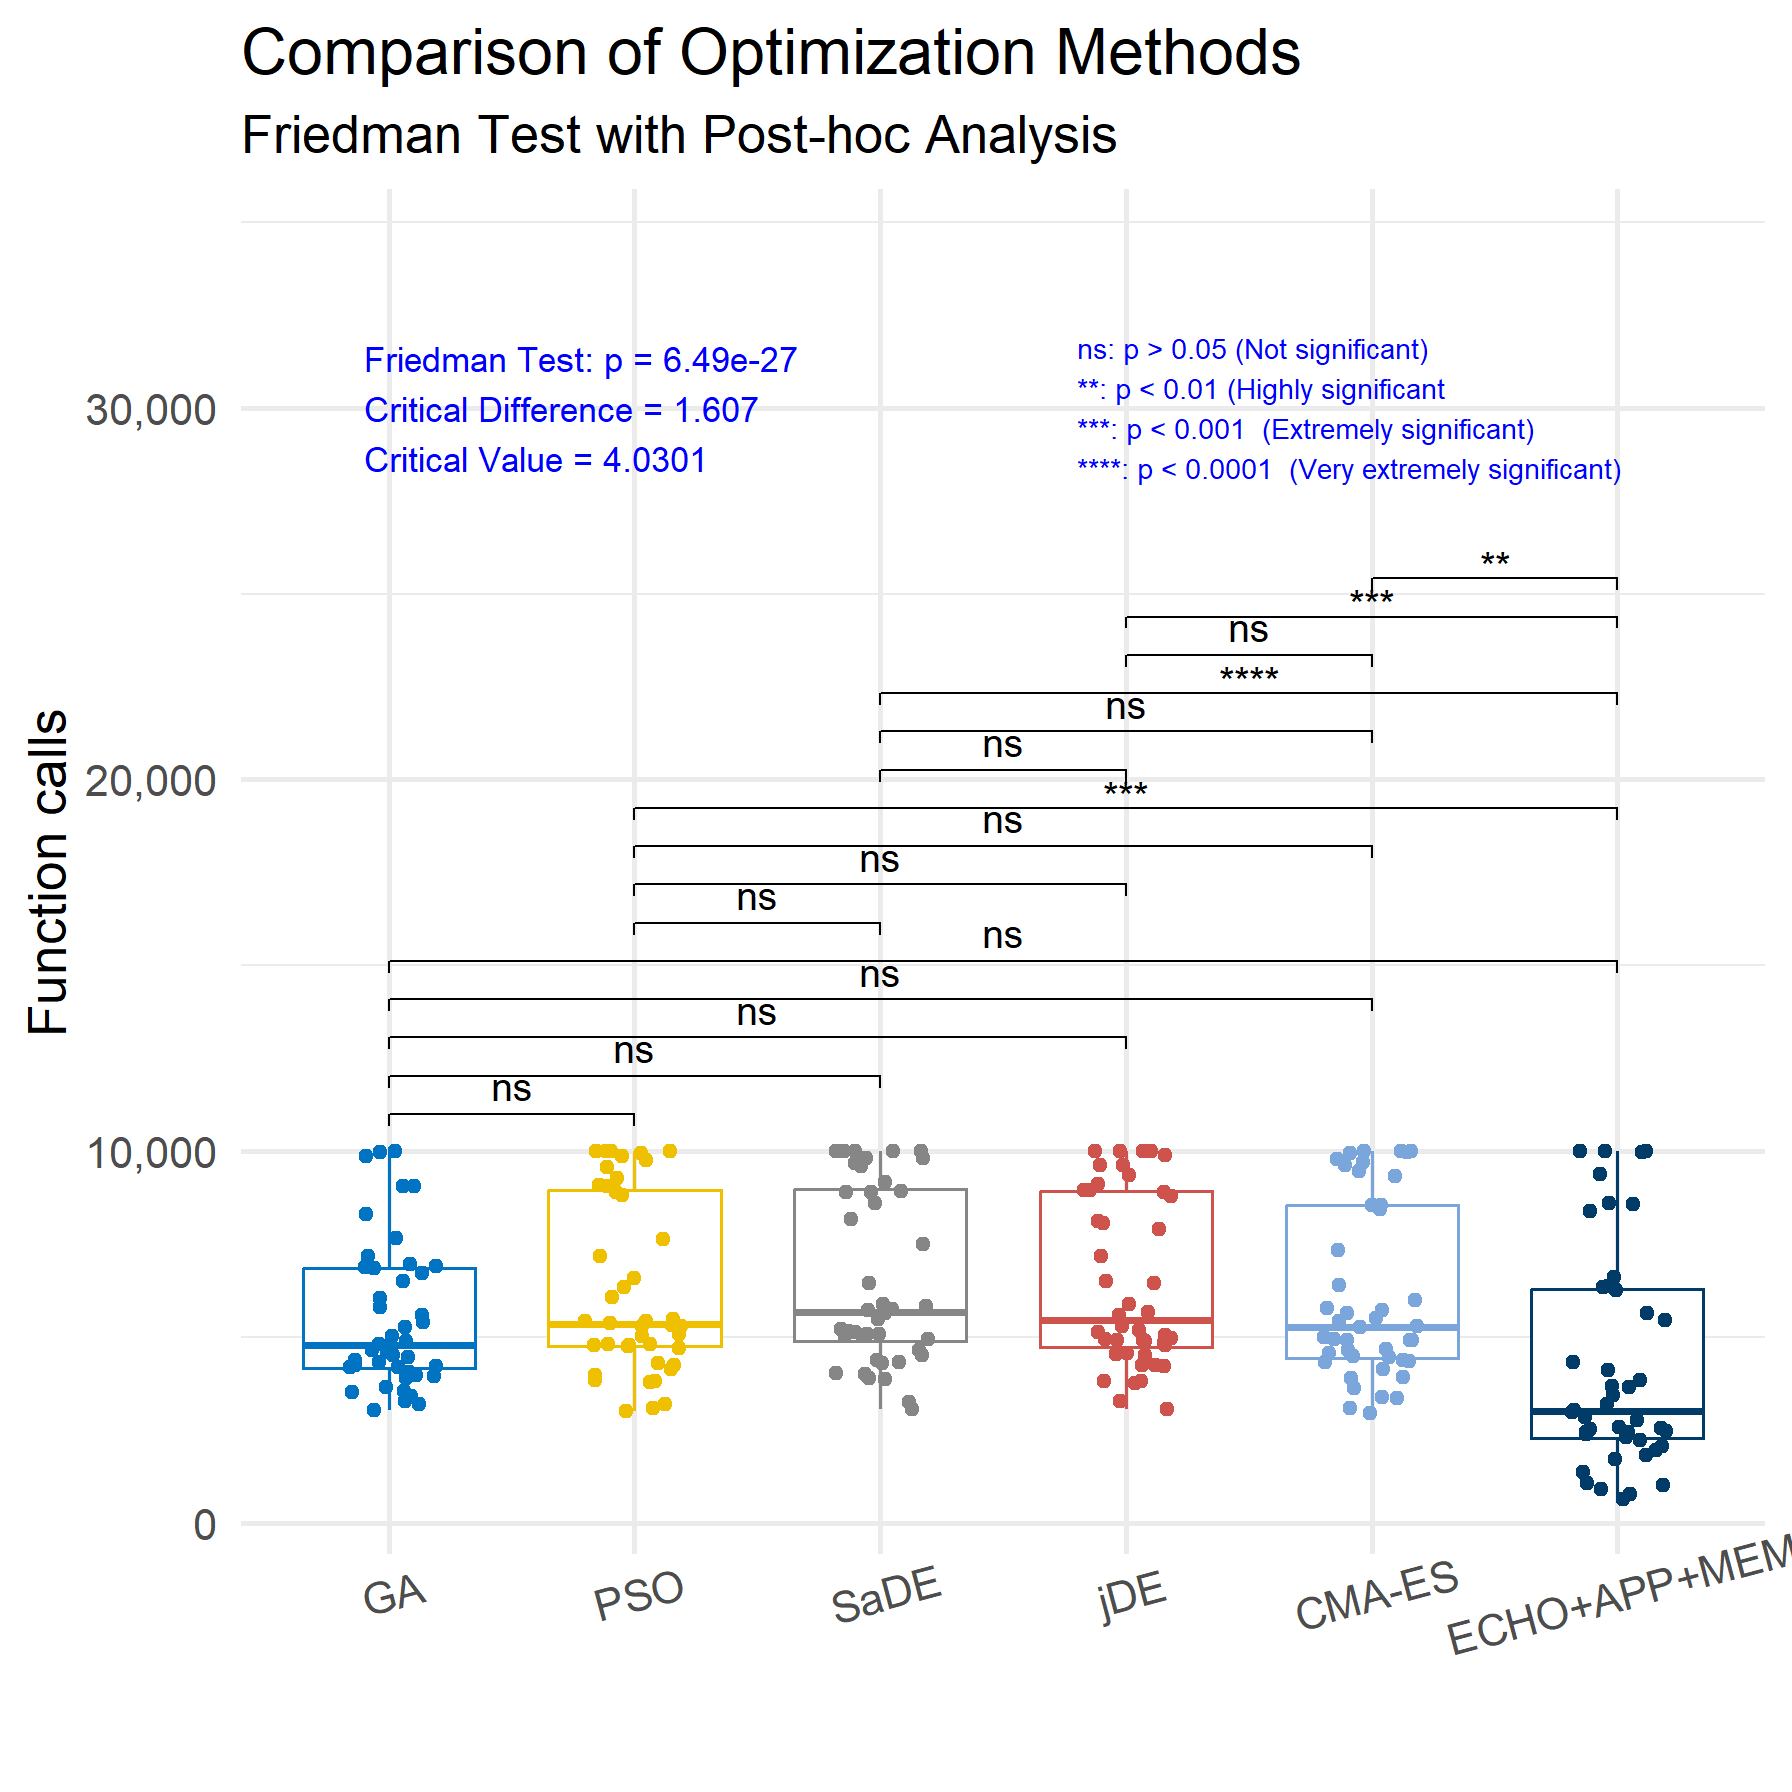
\includegraphics[scale=0.65]{pop200}

\caption{Statistical comparison of function calls of the different optimization
methods for low-dimensional benchmark functions\label{fig:statCalls200}}

\end{figure}

From the execution of the Friedman statistical test for comparing
the ECHO+APP+MEM method with other well-known optimization techniques,
a p-value of 6.49e-27 was obtained, indicating the presence of statistically
significant differences among the methods under study (Figure \ref{fig:statCalls200}).
The critical difference was calculated at 1.607, and the corresponding
critical value from the Tukey distribution was 4.03. These results
confirm that the overall ranking of the methods differs at a highly
significant level, thus justifying the need for a detailed post-hoc
pairwise analysis.

Focusing on the ECHO+APP+MEM method, the post-hoc results show that
its performance differs significantly from all other advanced techniques.
In particular, the comparison between the ECHO+APP+MEM method and
PSO reveals an extremely significant difference (p \textless{} 0.001),
while the difference with SaDE is marked as very extremely significant
(p \textless{} 0.0001). The comparison with jDE is also extremely
significant (p \textless{} 0.001), and with CMA-ES it is highly significant
(p \textless{} 0.01). On the other hand, the differences between the
other methods among themselves, as well as the differences between
GA and all other techniques (including the ECHO+APP+MEM method), were
found to be not statistically significant.

These findings suggest that ECHO+APP+MEM is able to outperform several
well-established and state-of-the-art optimization methods in a statistically
validated way. The strong statistical significance of the differences
observed with PSO, SaDE, jDE, and CMA-ES clearly highlights the superiority
of the ECHO+APP+MEM method in terms of both efficiency and reliability.
The lack of significant difference with GA may be attributed to the
high variability in GA’s performance, which, in many cases, is substantially
lower than that of the more advanced methods. Overall, the results
of the statistical analysis strengthen the validity of the experimental
evaluation and support the effectiveness of the ECHO+APP+MEM method
as a consistently strong approach across a wide range of optimization
problems.

{\footnotesize{}
\begin{table}[H]
{\footnotesize\caption{Comparison of function calls of the different optimization methods
for high-dimensional benchmark functions (population:50)\label{tab:callsHigh50}}
}{\footnotesize\par}
\centering{}{\footnotesize{}%
\begin{tabular}{|l|c|c|c|c|c|}
\hline 
{\footnotesize\textbf{FUNCTION}} & {\footnotesize\textbf{CLPSO}} & {\footnotesize\textbf{jDE}} & {\footnotesize\textbf{SaDE}} & {\footnotesize\textbf{CMA-ES}} & {\scriptsize\textbf{ECHO+APP+MEM}}\tabularnewline
\hline 
\hline 
{\footnotesize\textbf{DIFFERENTPOWERS50}} & {\footnotesize 2419} & {\footnotesize 1124} & {\footnotesize 2709} & {\footnotesize 1046} & {\footnotesize\textbf{\textcolor{green}{589}}}\tabularnewline
\hline 
{\footnotesize\textbf{DIFFERENTPOWERS100}} & {\footnotesize 2180} & {\footnotesize 1133} & {\footnotesize 1669} & {\footnotesize 1133} & {\footnotesize\textbf{\textcolor{green}{561}}}\tabularnewline
\hline 
{\footnotesize\textbf{DIFFERENTPOWERS150}} & {\footnotesize 2180} & {\footnotesize 1257} & {\footnotesize 1354} & {\footnotesize 1253} & {\footnotesize\textbf{\textcolor{green}{620}}}\tabularnewline
\hline 
{\footnotesize\textbf{DIFFERENTPOWERS200}} & {\footnotesize 2049} & {\footnotesize 1407} & {\footnotesize 1532} & {\footnotesize 1407} & {\footnotesize\textbf{\textcolor{green}{764}}}\tabularnewline
\hline 
{\footnotesize\textbf{DIFFERENTPOWERS250}} & {\footnotesize 2236} & {\footnotesize 1470} & {\footnotesize 1477} & {\footnotesize 1470} & {\footnotesize\textbf{\textcolor{green}{803}}}\tabularnewline
\hline 
{\footnotesize\textbf{DISCUS50}} & {\footnotesize 1729} & {\footnotesize\textbf{\textcolor{green}{719}}} & {\footnotesize 2082} & {\footnotesize 720} & {\footnotesize 1711}\tabularnewline
\hline 
{\footnotesize\textbf{DISCUS100}} & {\footnotesize 1929} & {\footnotesize\textbf{\textcolor{green}{719}}} & {\footnotesize 1028} & {\footnotesize\textbf{\textcolor{green}{719}}} & {\footnotesize 1694}\tabularnewline
\hline 
{\footnotesize\textbf{DISCUS150}} & {\footnotesize 1923} & {\footnotesize\textbf{\textcolor{green}{720}}} & {\footnotesize 943} & {\footnotesize 722} & {\footnotesize 1727}\tabularnewline
\hline 
{\footnotesize\textbf{DISCUS200}} & {\footnotesize 1384} & {\footnotesize\textbf{\textcolor{green}{721}}} & {\footnotesize 914} & {\footnotesize\textbf{\textcolor{green}{721}}} & {\footnotesize 1844}\tabularnewline
\hline 
{\footnotesize\textbf{DISCUS250}} & {\footnotesize 1413} & {\footnotesize\textbf{\textcolor{green}{721}}} & {\footnotesize 913} & {\footnotesize\textbf{\textcolor{green}{721}}} & {\footnotesize 1665}\tabularnewline
\hline 
{\footnotesize\textbf{ELLIPSOIDAL50}} & {\footnotesize 3336} & {\footnotesize\textbf{\textcolor{green}{888}}} & {\footnotesize 7532} & {\footnotesize 889} & {\footnotesize 3453}\tabularnewline
\hline 
{\footnotesize\textbf{ELLIPSOIDAL100}} & {\footnotesize 2959} & {\footnotesize\textbf{\textcolor{green}{1053}}} & {\footnotesize 5039} & {\footnotesize 1058} & {\footnotesize 4188}\tabularnewline
\hline 
{\footnotesize\textbf{ELLIPSOIDAL150}} & {\footnotesize 3114} & {\footnotesize\textbf{\textcolor{green}{1255}}} & {\footnotesize 4093} & {\footnotesize 1261} & {\footnotesize 4639}\tabularnewline
\hline 
{\footnotesize\textbf{ELLIPSOIDAL200}} & {\footnotesize 3031} & {\footnotesize\textbf{\textcolor{green}{1487}}} & {\footnotesize 3569} & {\footnotesize 1494} & {\footnotesize 4922}\tabularnewline
\hline 
{\footnotesize\textbf{ELLIPSOIDAL250}} & {\footnotesize 3339} & {\footnotesize 1729} & {\footnotesize 3074} & {\footnotesize\textbf{\textcolor{green}{1728}}} & {\footnotesize 5336}\tabularnewline
\hline 
{\footnotesize\textbf{EQUALMAXIMA50}} & {\footnotesize 1651} & {\footnotesize 1246} & {\footnotesize 2051} & {\footnotesize 724} & {\footnotesize\textbf{\textcolor{green}{545}}}\tabularnewline
\hline 
{\footnotesize\textbf{EQUALMAXIMA100}} & {\footnotesize 1776} & {\footnotesize 1297} & {\footnotesize 2228} & {\footnotesize 726} & {\footnotesize\textbf{\textcolor{green}{647}}}\tabularnewline
\hline 
{\footnotesize\textbf{EQUALMAXIMA150}} & {\footnotesize 1657} & {\footnotesize 1377} & {\footnotesize 2151} & {\footnotesize 728} & {\footnotesize\textbf{\textcolor{green}{727}}}\tabularnewline
\hline 
{\footnotesize\textbf{EQUALMAXIMA200}} & {\footnotesize 2003} & {\footnotesize 1424} & {\footnotesize 2359} & {\footnotesize\textbf{\textcolor{green}{729}}} & {\footnotesize 774}\tabularnewline
\hline 
{\footnotesize\textbf{EQUALMAXIMA250}} & {\footnotesize 1937} & {\footnotesize 1472} & {\footnotesize 2378} & {\footnotesize\textbf{\textcolor{green}{729}}} & {\footnotesize 822}\tabularnewline
\hline 
{\footnotesize\textbf{EXPONENTIAL50}} & {\footnotesize 2205} & {\footnotesize 1033} & {\footnotesize 4941} & {\footnotesize 748} & {\footnotesize\textbf{\textcolor{green}{95}}}\tabularnewline
\hline 
{\footnotesize\textbf{EXPONENTIAL100}} & {\footnotesize 1396} & {\footnotesize 747} & {\footnotesize 1033} & {\footnotesize 747} & {\footnotesize\textbf{\textcolor{green}{97}}}\tabularnewline
\hline 
{\footnotesize\textbf{EXPONENTIAL150}} & {\footnotesize 832} & {\footnotesize 751} & {\footnotesize 749} & {\footnotesize 753} & {\footnotesize\textbf{\textcolor{green}{101}}}\tabularnewline
\hline 
{\footnotesize\textbf{EXPONENTIAL200}} & {\footnotesize 803} & {\footnotesize 759} & {\footnotesize 755} & {\footnotesize 759} & {\footnotesize\textbf{\textcolor{green}{109}}}\tabularnewline
\hline 
{\footnotesize\textbf{EXPONENTIAL250}} & {\footnotesize 805} & {\footnotesize 759} & {\footnotesize 759} & {\footnotesize 759} & {\footnotesize\textbf{\textcolor{green}{109}}}\tabularnewline
\hline 
{\footnotesize\textbf{GRIEWANKROSENBROCK50}} & {\footnotesize 2314} & {\footnotesize 1237} & {\footnotesize 2730} & {\footnotesize 1168} & {\footnotesize\textbf{\textcolor{green}{562}}}\tabularnewline
\hline 
{\footnotesize\textbf{GRIEWANKROSENBROCK100}} & {\footnotesize 2323} & {\footnotesize 1352} & {\footnotesize 1438} & {\footnotesize 1332} & {\footnotesize\textbf{\textcolor{green}{574}}}\tabularnewline
\hline 
{\footnotesize\textbf{GRIEWANKROSENBROCK150}} & {\footnotesize 2239} & {\footnotesize 1452} & {\footnotesize 1490} & {\footnotesize 1427} & {\footnotesize\textbf{\textcolor{green}{642}}}\tabularnewline
\hline 
{\footnotesize\textbf{GRIEWANKROSENBROCK200}} & {\footnotesize 1976} & {\footnotesize 1640} & {\footnotesize 1675} & {\footnotesize 1609} & {\footnotesize\textbf{\textcolor{green}{824}}}\tabularnewline
\hline 
{\footnotesize\textbf{GRIEWANKROSENBROCK250}} & {\footnotesize 1903} & {\footnotesize 1683} & {\footnotesize 1683} & {\footnotesize 1658} & {\footnotesize\textbf{\textcolor{green}{907}}}\tabularnewline
\hline 
{\footnotesize\textbf{ROSENBROCK50}} & {\footnotesize 2384} & {\footnotesize 1160} & {\footnotesize 2256} & {\footnotesize\textbf{\textcolor{green}{1083}}} & {\footnotesize 4610}\tabularnewline
\hline 
{\footnotesize\textbf{ROSENBROCK100}} & {\footnotesize 2043} & {\footnotesize 1329} & {\footnotesize 1412} & {\footnotesize\textbf{\textcolor{green}{1311}}} & {\footnotesize 5856}\tabularnewline
\hline 
{\footnotesize\textbf{ROSENBROCK150}} & {\footnotesize 2077} & {\footnotesize 1555} & {\footnotesize 1580} & {\footnotesize\textbf{\textcolor{green}{1535}}} & {\footnotesize 6601}\tabularnewline
\hline 
{\footnotesize\textbf{ROSENBROCK200}} & {\footnotesize 2023} & {\footnotesize 1766} & {\footnotesize 1775} & {\footnotesize\textbf{\textcolor{green}{1741}}} & {\footnotesize 7141}\tabularnewline
\hline 
{\footnotesize\textbf{ROSENBROCK250}} & {\footnotesize 2388} & {\footnotesize 2025} & {\footnotesize 2025} & {\footnotesize\textbf{\textcolor{green}{2002}}} & {\footnotesize 6813}\tabularnewline
\hline 
{\footnotesize\textbf{SHARPRIDGE50}} & {\footnotesize 2561} & {\footnotesize 964} & {\footnotesize 5340} & {\footnotesize 861} & {\footnotesize\textbf{\textcolor{green}{437(0.96)}}}\tabularnewline
\hline 
{\footnotesize\textbf{SHARPRIDGE100}} & {\footnotesize 1738} & {\footnotesize 858} & {\footnotesize 1760} & {\footnotesize 853} & {\footnotesize\textbf{\textcolor{green}{414}}}\tabularnewline
\hline 
{\footnotesize\textbf{SHARPRIDGE150}} & {\footnotesize 1609} & {\footnotesize 881(0.96)} & {\footnotesize 1273} & {\footnotesize 871} & {\footnotesize\textbf{\textcolor{green}{435}}}\tabularnewline
\hline 
{\footnotesize\textbf{SHARPRIDGE200}} & {\footnotesize 1287} & {\footnotesize 883} & {\footnotesize 1161} & {\footnotesize 883} & {\footnotesize\textbf{\textcolor{green}{607}}}\tabularnewline
\hline 
{\footnotesize\textbf{SHARPRIDGE250}} & {\footnotesize 1414(0.96)} & {\footnotesize 880} & {\footnotesize 1110} & {\footnotesize 884} & {\footnotesize\textbf{\textcolor{green}{610}}}\tabularnewline
\hline 
{\footnotesize\textbf{SINUSOIDAL50}} & {\footnotesize 2403(0.5)} & {\footnotesize 919(0.3)} & {\footnotesize 1007(0.3)} & {\footnotesize 930(0.6)} & {\footnotesize\textbf{\textcolor{green}{271(0.3)}}}\tabularnewline
\hline 
{\footnotesize\textbf{SINUSOIDAL100}} & {\footnotesize 1155(0)} & {\footnotesize 899(0)} & {\footnotesize 1451(0.6)} & {\footnotesize 898(0.3)} & {\footnotesize\textbf{\textcolor{green}{249(0)}}}\tabularnewline
\hline 
{\footnotesize\textbf{SINUSOIDAL150}} & {\footnotesize 753(0)} & {\footnotesize 703(0)} & {\footnotesize 703(0)} & {\footnotesize 708(0.3)} & {\footnotesize\textbf{\textcolor{green}{53(0)}}}\tabularnewline
\hline 
{\footnotesize\textbf{SINUSOIDAL200}} & {\footnotesize 753(0)} & {\footnotesize 703(0)} & {\footnotesize 703(0)} & {\footnotesize 703(0)} & {\footnotesize\textbf{\textcolor{green}{53(0)}}}\tabularnewline
\hline 
{\footnotesize\textbf{SINUSOIDAL250}} & {\footnotesize 753(0)} & {\footnotesize 703(0)} & {\footnotesize 703(0)} & {\footnotesize 703(0)} & {\footnotesize\textbf{\textcolor{green}{53(0)}}}\tabularnewline
\hline 
{\footnotesize\textbf{ZAKHAROV50}} & {\footnotesize 1623} & {\footnotesize 803} & {\footnotesize 1254} & {\footnotesize 866} & {\footnotesize\textbf{\textcolor{green}{550}}}\tabularnewline
\hline 
{\footnotesize\textbf{ZAKHAROV100}} & {\footnotesize 1742} & {\footnotesize 876} & {\footnotesize 1433} & {\footnotesize 920} & {\footnotesize\textbf{\textcolor{green}{631}}}\tabularnewline
\hline 
{\footnotesize\textbf{ZAKHAROV150}} & {\footnotesize 1792} & {\footnotesize 920} & {\footnotesize 1558} & {\footnotesize 990} & {\footnotesize\textbf{\textcolor{green}{849}}}\tabularnewline
\hline 
{\footnotesize\textbf{ZAKHAROV200}} & {\footnotesize 1842} & {\footnotesize 961} & {\footnotesize 1769} & {\footnotesize 1014} & {\footnotesize\textbf{\textcolor{green}{933}}}\tabularnewline
\hline 
{\footnotesize\textbf{ZAKHAROV250}} & {\footnotesize 1816} & {\footnotesize\textbf{\textcolor{green}{960}}} & {\footnotesize 1795} & {\footnotesize 1338} & {\footnotesize 969}\tabularnewline
\hline 
{\footnotesize\textbf{TOTAL}} & {\footnotesize\textbf{95,197(0.9)}} & {\footnotesize\textbf{55,380(0.9)}} & {\footnotesize\textbf{98,416(0.9)}} & {\footnotesize\textbf{\textcolor{green}{52,032(0.9)}}} & {\footnotesize\textbf{80,186(0.9)}}\tabularnewline
\hline 
\end{tabular}}{\footnotesize\par}
\end{table}
}{\footnotesize\par}

From Table \ref{tab:callsHigh50}, which provides a comparative analysis
of high-dimensional functions (ranging from 50 to 250 dimensions),
important conclusions can be drawn regarding the performance of the
ECHO+APP+MEM method against contemporary optimization benchmarks.
The ECHO+APP+MEM method records a total of 80,186 objective function
calls, with a success rate of 90\%. This performance places it between
jDE (55,380 calls) and CMA-ES (52,032 calls), but it stands out for
its remarkable efficiency on specific types of problems.

In several key categories of functions, the ECHO+APP+MEM method demonstrates
clear superiority. In exponential-type functions (EXPONENTIAL), it
achieves dramatically fewer function calls. For example, in EXPONENTIAL50
it requires only 95 calls, compared to 2205 for CLPSO, 1033 for jDE,
and 4941 for SaDE. A similar pattern is observed across other dimensions
(EXPONENTIAL100--250), where the ECHO+APP+MEM method never exceeds
109 calls, while the competing algorithms often require more than
700. This showcases the method’s ability to rapidly locate global
minima in smooth landscapes.

In functions with many local minima, such as SHARPRIDGE and SINUSOIDAL,
the ECHO+APP+MEM method maintains competitive performance. In SHARPRIDGE50,
it reaches the optimum with 437 calls and a 96\% success rate, outperforming
CMA-ES (861 calls) and SaDE (5340 calls). In the SINUSOIDAL functions,
although all methods demonstrate low success rates (0--30\%), the
ECHO+APP+MEM method consistently requires the fewest calls for example,
53 calls for SINUSOIDAL150 compared to 753 for CLPSO. This indicates
strong efficiency even in rugged landscapes where exact success is
hard to achieve.

However, in some more demanding functions such as ROSENBROCK and ELLIPSOIDAL,
the ECHO+APP+MEM method exhibits higher computational cost. In ROSENBROCK250,
it requires 6813 calls, significantly more than jDE (2025 calls) and
CMA-ES (2002 calls). A similar pattern appears in the ELLIPSOIDAL
functions, where, for 250 dimensions, it needs 5336 calls about three
times more than CMA-ES (1728 calls). This suggests that in problems
characterized by strong curvature, the method may require more iterations
to converge.

Overall, with an average success rate of 90\%, the ECHO+APP+MEM method
maintains reliable accuracy, even though in some cases it lags behind
jDE and CMA-ES in convergence speed. Its ability to drastically reduce
function calls in exponential and non-convex functions (such as SHARPRIDGE)
makes it particularly suitable for problems with wide attraction basins
or numerous shallow local minima. Nevertheless, improving its performance
on high-curvature functions (e.g., ROSENBROCK-type problems) remains
a potential direction for future enhancement.

\begin{figure}[H]
\begin{centering}
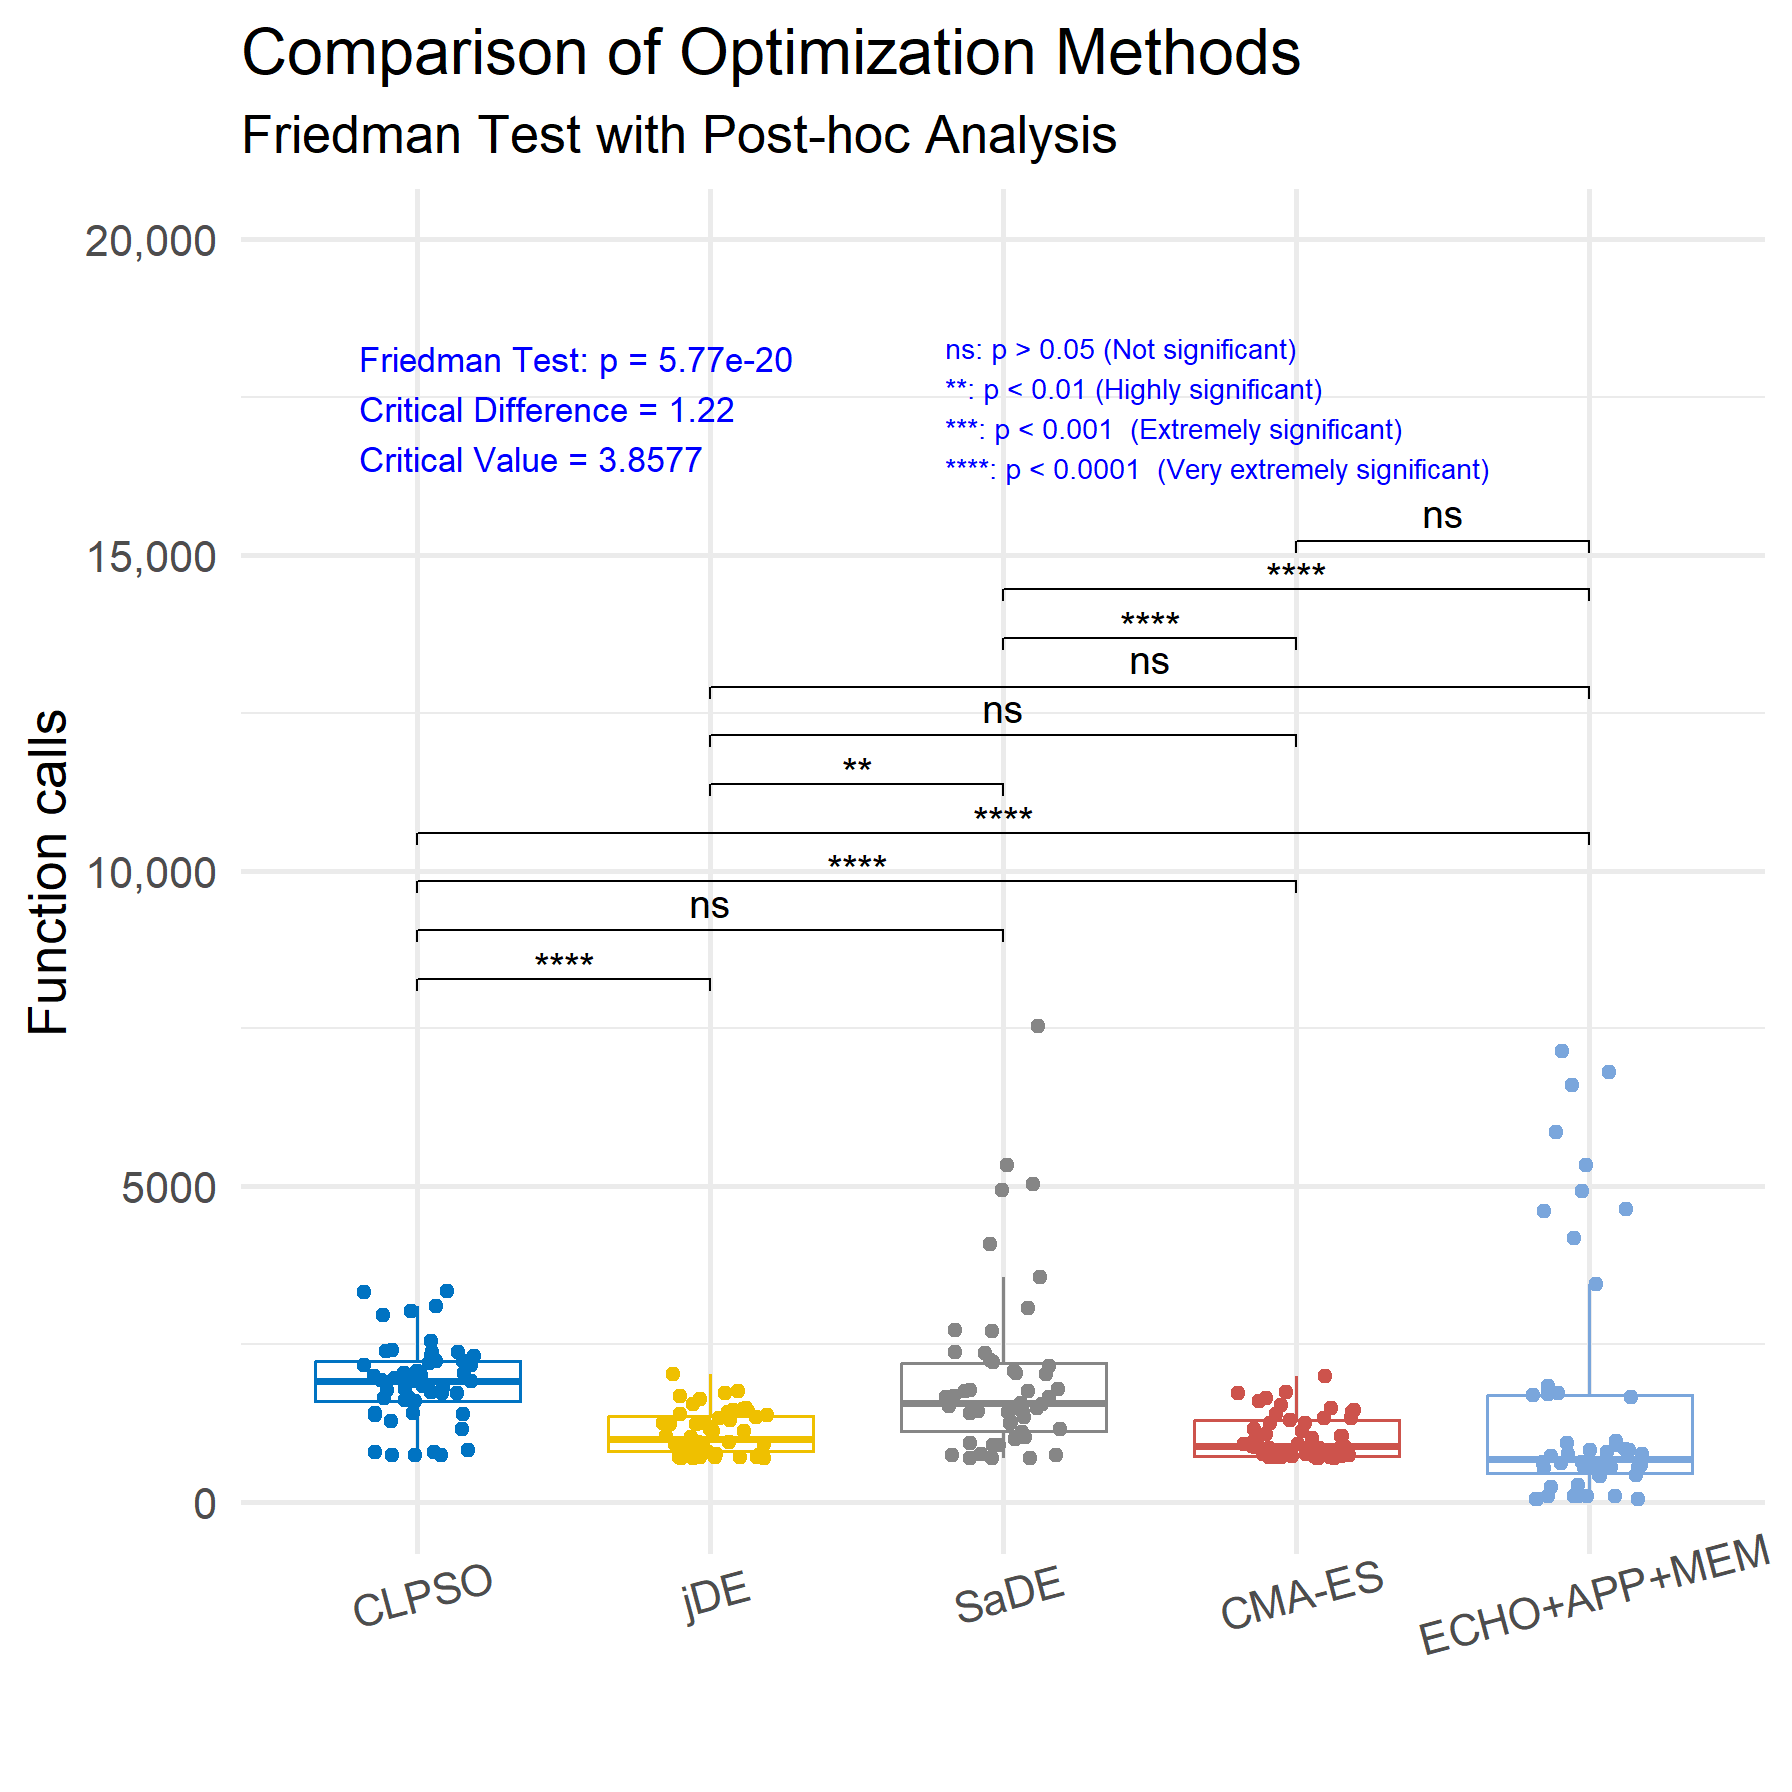
\includegraphics[scale=0.65]{pop50}
\par\end{centering}
\caption{Statistical comparison of function calls of the different optimization
methods for high-dimensional benchmark functions (population: 50)
\label{fig:statCallsPop50}}
\end{figure}

In Figure \ref{fig:statCallsPop50}, the Friedman test reported a
p-value of 5.77e-20, indicating statistically significant differences
among the optimization methods. The critical difference was calculated
as 1.22, with a corresponding critical value of 3.85. The ECHO+APP+MEM
method showed very extremely significant differences compared to CLPSO
(p \textless{} 0.0001) and SaDE (p \textless{} 0.0001), confirming
its superiority over these methods. No statistically significant difference
was observed when compared to jDE and CMA-ES, suggesting that its
performance is comparable to these more advanced approaches. Overall,
the analysis highlights the ECHO+APP+MEM method as clearly superior
to simpler techniques such as CLPSO and SaDE, while maintaining equivalent
performance to established methods like jDE and CMA-ES, reinforcing
its reliability and competitiveness in optimization problems using
a population size of 50.

\begin{table}[H]
\caption{Comparison of function calls of the different optimization methods
for high-dimensional benchmark functions $Np=4+\left\lfloor 3\cdot\log(\text{dimension})\right\rfloor $\label{tab:callsHighFormula}}

\centering{}{\footnotesize{}%
\begin{tabular}{|l|c|c|c|c|c|}
\hline 
{\footnotesize\textbf{FUNCTION}} & {\footnotesize\textbf{CLPSO}} & {\footnotesize\textbf{jDE}} & {\footnotesize\textbf{SaDE}} & {\footnotesize\textbf{CMA-ES}} & {\footnotesize\textbf{ECHO+APP+MEM}}\tabularnewline
\hline 
\hline 
{\footnotesize\textbf{DIFFERENTPOWERS50}} & {\footnotesize 877} & {\footnotesize 537} & {\footnotesize 1871} & {\footnotesize 555} & {\footnotesize\textbf{\textcolor{green}{362}}}\tabularnewline
\hline 
{\footnotesize\textbf{DIFFERENTPOWERS100}} & {\footnotesize 1002} & {\footnotesize 746} & {\footnotesize 1071} & {\footnotesize 740} & {\footnotesize\textbf{\textcolor{green}{492}}}\tabularnewline
\hline 
{\footnotesize\textbf{DIFFERENTPOWERS150}} & {\footnotesize 1061} & {\footnotesize 837} & {\footnotesize 1037} & {\footnotesize 834} & {\footnotesize\textbf{\textcolor{green}{617}}}\tabularnewline
\hline 
{\footnotesize\textbf{DIFFERENTPOWERS200}} & {\footnotesize 1102} & {\footnotesize 986} & {\footnotesize 1037} & {\footnotesize 985} & {\footnotesize\textbf{\textcolor{green}{723}}}\tabularnewline
\hline 
{\footnotesize\textbf{DIFFERENTPOWERS250}} & {\footnotesize 1281} & {\footnotesize 1077} & {\footnotesize 1104} & {\footnotesize 1073} & {\footnotesize\textbf{\textcolor{green}{821}}}\tabularnewline
\hline 
{\footnotesize\textbf{DISCUS50}} & {\footnotesize 635} & {\footnotesize\textbf{\textcolor{green}{238}}} & {\footnotesize 1252} & {\footnotesize 232} & {\footnotesize 397}\tabularnewline
\hline 
{\footnotesize\textbf{DISCUS100}} & {\footnotesize 588} & {\footnotesize\textbf{\textcolor{green}{259}}} & {\footnotesize 962} & {\footnotesize 259} & {\footnotesize 451}\tabularnewline
\hline 
{\footnotesize\textbf{DISCUS150}} & {\footnotesize 523} & {\footnotesize\textbf{\textcolor{green}{287}}} & {\footnotesize 628} & {\footnotesize 287} & {\footnotesize 563}\tabularnewline
\hline 
{\footnotesize\textbf{DISCUS200}} & {\footnotesize 559} & {\footnotesize\textbf{\textcolor{green}{287}}} & {\footnotesize 470} & {\footnotesize 287} & {\footnotesize 584}\tabularnewline
\hline 
{\footnotesize\textbf{DISCUS250}} & {\footnotesize 694} & {\footnotesize\textbf{\textcolor{green}{302}}} & {\footnotesize 451} & {\footnotesize\textbf{\textcolor{green}{302}}} & {\footnotesize 630}\tabularnewline
\hline 
{\footnotesize\textbf{ELLIPSOIDAL50}} & {\footnotesize 1255} & {\footnotesize 405} & {\footnotesize 3061} & {\footnotesize\textbf{\textcolor{green}{395}}} & {\footnotesize 1297}\tabularnewline
\hline 
{\footnotesize\textbf{ELLIPSOIDAL100}} & {\footnotesize 1394} & {\footnotesize\textbf{\textcolor{green}{588}}} & {\footnotesize 3098} & {\footnotesize 593} & {\footnotesize 1820}\tabularnewline
\hline 
{\footnotesize\textbf{ELLIPSOIDAL150}} & {\footnotesize 1463} & {\footnotesize\textbf{\textcolor{green}{876}}} & {\footnotesize 2699} & {\footnotesize 881} & {\footnotesize 2206}\tabularnewline
\hline 
{\footnotesize\textbf{ELLIPSOIDAL200}} & {\footnotesize 1532} & {\footnotesize\textbf{\textcolor{green}{1030}}} & {\footnotesize 2686} & {\footnotesize 1041} & {\footnotesize 2505}\tabularnewline
\hline 
{\footnotesize\textbf{ELLIPSOIDAL250}} & {\footnotesize 1728} & {\footnotesize\textbf{\textcolor{green}{1344}}} & {\footnotesize 2673} & {\footnotesize 1346} & {\footnotesize 2790}\tabularnewline
\hline 
{\footnotesize\textbf{EQUALMAXIMA50}} & {\footnotesize 866} & {\footnotesize 726} & {\footnotesize 914} & {\footnotesize\textbf{\textcolor{green}{219}}} & {\footnotesize 513}\tabularnewline
\hline 
{\footnotesize\textbf{EQUALMAXIMA100}} & {\footnotesize 1033} & {\footnotesize 824} & {\footnotesize 1096} & {\footnotesize\textbf{\textcolor{green}{249}}} & {\footnotesize 603}\tabularnewline
\hline 
{\footnotesize\textbf{EQUALMAXIMA150}} & {\footnotesize 1090} & {\footnotesize 961} & {\footnotesize 1215} & {\footnotesize\textbf{\textcolor{green}{279}}} & {\footnotesize 714}\tabularnewline
\hline 
{\footnotesize\textbf{EQUALMAXIMA200}} & {\footnotesize 1184} & {\footnotesize 988} & {\footnotesize 1356} & {\footnotesize\textbf{\textcolor{green}{279}}} & {\footnotesize 741}\tabularnewline
\hline 
{\footnotesize\textbf{EQUALMAXIMA250}} & {\footnotesize 1235} & {\footnotesize 1054} & {\footnotesize 1371} & {\footnotesize\textbf{\textcolor{green}{294}}} & {\footnotesize 794}\tabularnewline
\hline 
{\footnotesize\textbf{EXPONENTIAL50}} & {\footnotesize 727} & {\footnotesize 481} & {\footnotesize 2402} & {\footnotesize 254} & {\footnotesize\textbf{\textcolor{green}{59}}}\tabularnewline
\hline 
{\footnotesize\textbf{EXPONENTIAL100}} & {\footnotesize 590} & {\footnotesize 285} & {\footnotesize 883} & {\footnotesize 285} & {\footnotesize\textbf{\textcolor{green}{64}}}\tabularnewline
\hline 
{\footnotesize\textbf{EXPONENTIAL150}} & {\footnotesize 335} & {\footnotesize 317} & {\footnotesize 317} & {\footnotesize 317} & {\footnotesize\textbf{\textcolor{green}{70}}}\tabularnewline
\hline 
{\footnotesize\textbf{EXPONENTIAL200}} & {\footnotesize 336} & {\footnotesize 325} & {\footnotesize 323} & {\footnotesize 325} & {\footnotesize\textbf{\textcolor{green}{78}}}\tabularnewline
\hline 
{\footnotesize\textbf{EXPONENTIAL250}} & {\footnotesize 355} & {\footnotesize 340} & {\footnotesize 339} & {\footnotesize 339} & {\footnotesize\textbf{\textcolor{green}{80}}}\tabularnewline
\hline 
{\footnotesize\textbf{GRIEWANKROSENBROCK50}} & {\footnotesize 1119} & {\footnotesize 813} & {\footnotesize 1598} & {\footnotesize 711} & {\footnotesize\textbf{\textcolor{green}{370}}}\tabularnewline
\hline 
{\footnotesize\textbf{GRIEWANKROSENBROCK100}} & {\footnotesize 1084} & {\footnotesize 886} & {\footnotesize 990} & {\footnotesize 870} & {\footnotesize\textbf{\textcolor{green}{503}}}\tabularnewline
\hline 
{\footnotesize\textbf{GRIEWANKROSENBROCK150}} & {\footnotesize 1237} & {\footnotesize 1054} & {\footnotesize 1088} & {\footnotesize 1030} & {\footnotesize\textbf{\textcolor{green}{513}}}\tabularnewline
\hline 
{\footnotesize\textbf{GRIEWANKROSENBROCK200}} & {\footnotesize 1265} & {\footnotesize 1208} & {\footnotesize 1234} & {\footnotesize 1187} & {\footnotesize\textbf{\textcolor{green}{704}}}\tabularnewline
\hline 
{\footnotesize\textbf{GRIEWANKROSENBROCK250}} & {\footnotesize 1359} & {\footnotesize 1264} & {\footnotesize 1267} & {\footnotesize 1239} & {\footnotesize\textbf{\textcolor{green}{856}}}\tabularnewline
\hline 
{\footnotesize\textbf{ROSENBROCK50}} & {\footnotesize 922} & {\footnotesize 632} & {\footnotesize 1546} & {\footnotesize\textbf{\textcolor{green}{592}}} & {\footnotesize 1896}\tabularnewline
\hline 
{\footnotesize\textbf{ROSENBROCK100}} & {\footnotesize 1102} & {\footnotesize 855} & {\footnotesize 971} & {\footnotesize\textbf{\textcolor{green}{841}}} & {\footnotesize 2510}\tabularnewline
\hline 
{\footnotesize\textbf{ROSENBROCK150}} & {\footnotesize 1313} & {\footnotesize 1123} & {\footnotesize 1136} & {\footnotesize\textbf{\textcolor{green}{1104}}} & {\footnotesize 3116}\tabularnewline
\hline 
{\footnotesize\textbf{ROSENBROCK200}} & {\footnotesize 1493} & {\footnotesize 1339} & {\footnotesize 1362} & {\footnotesize\textbf{\textcolor{green}{1314}}} & {\footnotesize 3430}\tabularnewline
\hline 
{\footnotesize\textbf{ROSENBROCK250}} & {\footnotesize 1731} & {\footnotesize 1594} & {\footnotesize 1601} & {\footnotesize\textbf{\textcolor{green}{1568}}} & {\footnotesize 3628}\tabularnewline
\hline 
{\footnotesize\textbf{SHARPRIDGE50}} & {\footnotesize 830} & {\footnotesize 503} & {\footnotesize 2443(0.96)} & {\footnotesize 379} & {\footnotesize\textbf{\textcolor{green}{275}}}{\footnotesize\textcolor{green}{(0.96)}}\tabularnewline
\hline 
{\footnotesize\textbf{SHARPRIDGE100}} & {\footnotesize 1741} & {\footnotesize 424(0.96)} & {\footnotesize 1789} & {\footnotesize 419(0.96)} & {\footnotesize\textbf{\textcolor{green}{267}}}\tabularnewline
\hline 
{\footnotesize\textbf{SHARPRIDGE150}} & {\footnotesize 630} & {\footnotesize 434(0.96)} & {\footnotesize 1128(0.96)} & {\footnotesize 427(0.96)} & {\footnotesize\textbf{\textcolor{green}{259}}}\tabularnewline
\hline 
{\footnotesize\textbf{SHARPRIDGE200}} & {\footnotesize 697} & {\footnotesize 438} & {\footnotesize 867} & {\footnotesize 437} & {\footnotesize\textbf{\textcolor{green}{291}}}\tabularnewline
\hline 
{\footnotesize\textbf{SHARPRIDGE250}} & {\footnotesize 569(0.93)} & {\footnotesize 422(0.96)} & {\footnotesize 841} & {\footnotesize 426(0.96)} & {\footnotesize\textbf{\textcolor{green}{265}}}{\footnotesize\textcolor{green}{(0.96)}}\tabularnewline
\hline 
{\footnotesize\textbf{SINUSOIDAL50}} & {\footnotesize 529(0.1)} & {\footnotesize 441(0)} & {\footnotesize 490(0)} & {\footnotesize 436(0)} & {\footnotesize\textbf{\textcolor{green}{224}}}{\footnotesize\textcolor{green}{(0)}}\tabularnewline
\hline 
{\footnotesize\textbf{SINUSOIDAL100}} & {\footnotesize 747(0)} & {\footnotesize 370(0)} & {\footnotesize 801(0)} & {\footnotesize 370(0)} & {\footnotesize\textbf{\textcolor{green}{149}}}{\footnotesize\textcolor{green}{(0)}}\tabularnewline
\hline 
{\footnotesize\textbf{SINUSOIDAL150}} & {\footnotesize 288(0)} & {\footnotesize 269(0)} & {\footnotesize 269(0)} & {\footnotesize 269(0)} & {\footnotesize\textbf{\textcolor{green}{22}}}{\footnotesize\textcolor{green}{(0)}}\tabularnewline
\hline 
{\footnotesize\textbf{SINUSOIDAL200}} & {\footnotesize 288(0)} & {\footnotesize 269(0)} & {\footnotesize 269(0)} & {\footnotesize 269(0)} & {\footnotesize\textbf{\textcolor{green}{22}}}{\footnotesize\textcolor{green}{(0)}}\tabularnewline
\hline 
{\footnotesize\textbf{SINUSOIDAL250}} & {\footnotesize 303(0)} & {\footnotesize 283(0)} & {\footnotesize 283(0)} & {\footnotesize 283(0)} & {\footnotesize\textbf{\textcolor{green}{23}}}{\footnotesize\textcolor{green}{(0)}}\tabularnewline
\hline 
{\footnotesize\textbf{ZAKHAROV50}} & {\footnotesize 483} & {\footnotesize 323} & {\footnotesize 475} & {\footnotesize 352} & {\footnotesize\textbf{\textcolor{green}{325}}}\tabularnewline
\hline 
{\footnotesize\textbf{ZAKHAROV100}} & {\footnotesize 604} & {\footnotesize 416} & {\footnotesize 693} & {\footnotesize\textbf{\textcolor{green}{413}}} & {\footnotesize 487}\tabularnewline
\hline 
{\footnotesize\textbf{ZAKHAROV150}} & {\footnotesize 713} & {\footnotesize 487} & {\footnotesize 817} & {\footnotesize\textbf{\textcolor{green}{504}}} & {\footnotesize 486}\tabularnewline
\hline 
{\footnotesize\textbf{ZAKHAROV200}} & {\footnotesize 750} & {\footnotesize\textbf{\textcolor{green}{528}}} & {\footnotesize 821} & {\footnotesize 579} & {\footnotesize 663}\tabularnewline
\hline 
{\footnotesize\textbf{ZAKHAROV250}} & {\footnotesize 885} & {\footnotesize 538} & {\footnotesize 893} & {\footnotesize 693} & {\footnotesize\textbf{\textcolor{green}{501}}}\tabularnewline
\hline 
{\footnotesize\textbf{TOTAL}} & {\footnotesize\textbf{46,127(0.9)}} & {\footnotesize\textbf{33,013(0.89)}} & {\footnotesize\textbf{59,988(0.89)}} & {\footnotesize\textbf{\textcolor{green}{29,362(0.89)}}} & {\footnotesize\textbf{41,759(0.89)}}\tabularnewline
\hline 
\end{tabular}}{\footnotesize\par}
\end{table}

Table \ref{tab:callsHighFormula} presents the comparative performance
of the ECHO+APP+MEM method against other modern optimization techniques
on high-dimensional problems (ranging from 50 to 250 dimensions),
where the population size is determined dynamically according to the
formula: $Np=4+\left\lfloor 3\cdot\log(\text{dimension})\right\rfloor $.
The first row lists the methods under comparison: CLPSO, jDE, SaDE,
CMA-ES, and the ECHO+APP+MEM method. The first column contains the
test functions used in the evaluation, while the table entries report
the number of objective function calls required to reach an acceptable
solution. In some cases, the success rate is also indicated in parentheses,
showing the percentage of runs in which the global minimum was successfully
found.

The overall performance of the ECHO+APP+MEM method is highly satisfactory,
with a total of 41,759 calls and an average success rate of 89\%,
comparable to the other methods. jDE and CMA-ES achieve slightly fewer
total calls (33,013 and 29,362 respectively), but in many individual
cases the ECHO+APP+MEM method converges more quickly. For example,
in the EXPONENTIAL150 to EXPONENTIAL250 functions, the ECHO+APP+MEM
method requires only 70 to 80 calls, outperforming or matching the
most efficient competitors. A similar trend is seen in the SINUSOIDAL
functions, where all methods exhibit low success rates, yet the ECHO+APP+MEM
method consistently requires far fewer calls only 22 or 23, compared
to 269 and above for the others.

In the SHARPRIDGE functions, the ECHO+APP+MEM method shows very strong
performance with low function evaluations and high success rates.
For instance, in SHARPRIDGE250, it needs only 265 calls with a 96\%
success rate, while jDE and CMA-ES require more than 420 calls. This
suggests an effective handling of rugged landscapes with many local
minima and abrupt variations.

However, in more demanding functions such as ROSENBROCK and ELLIPSOIDAL,
the ECHO+APP+MEM method shows higher computational cost compared to
its competitors. In ROSENBROCK250, for example, it requires 3628 calls,
while jDE and CMA-ES achieve similar results in approximately 2000
calls. A similar pattern appears in ELLIPSOIDAL250, where the ECHO+APP+MEM
method requires 2790 calls compared to roughly 1340 for CMA-ES. This
indicates that for problems characterized by high curvature or strong
inter-variable dependencies, the ECHO+APP+MEM method may require more
iterations to converge.

Overall, the results in this table suggest that the ECHO+APP+MEM method
is particularly effective in problems with broad attraction basins,
many local optima, or non-convex structures, as it manages to reach
good solutions with relatively few function evaluations. In contrast,
it may need more effort for convergence in problems with pronounced
curvature. Nevertheless, its high success rate and the consistent
stability across various problem types make it a competitive and robust
choice for high-dimensional optimization tasks.

\begin{figure}[H]
\begin{centering}
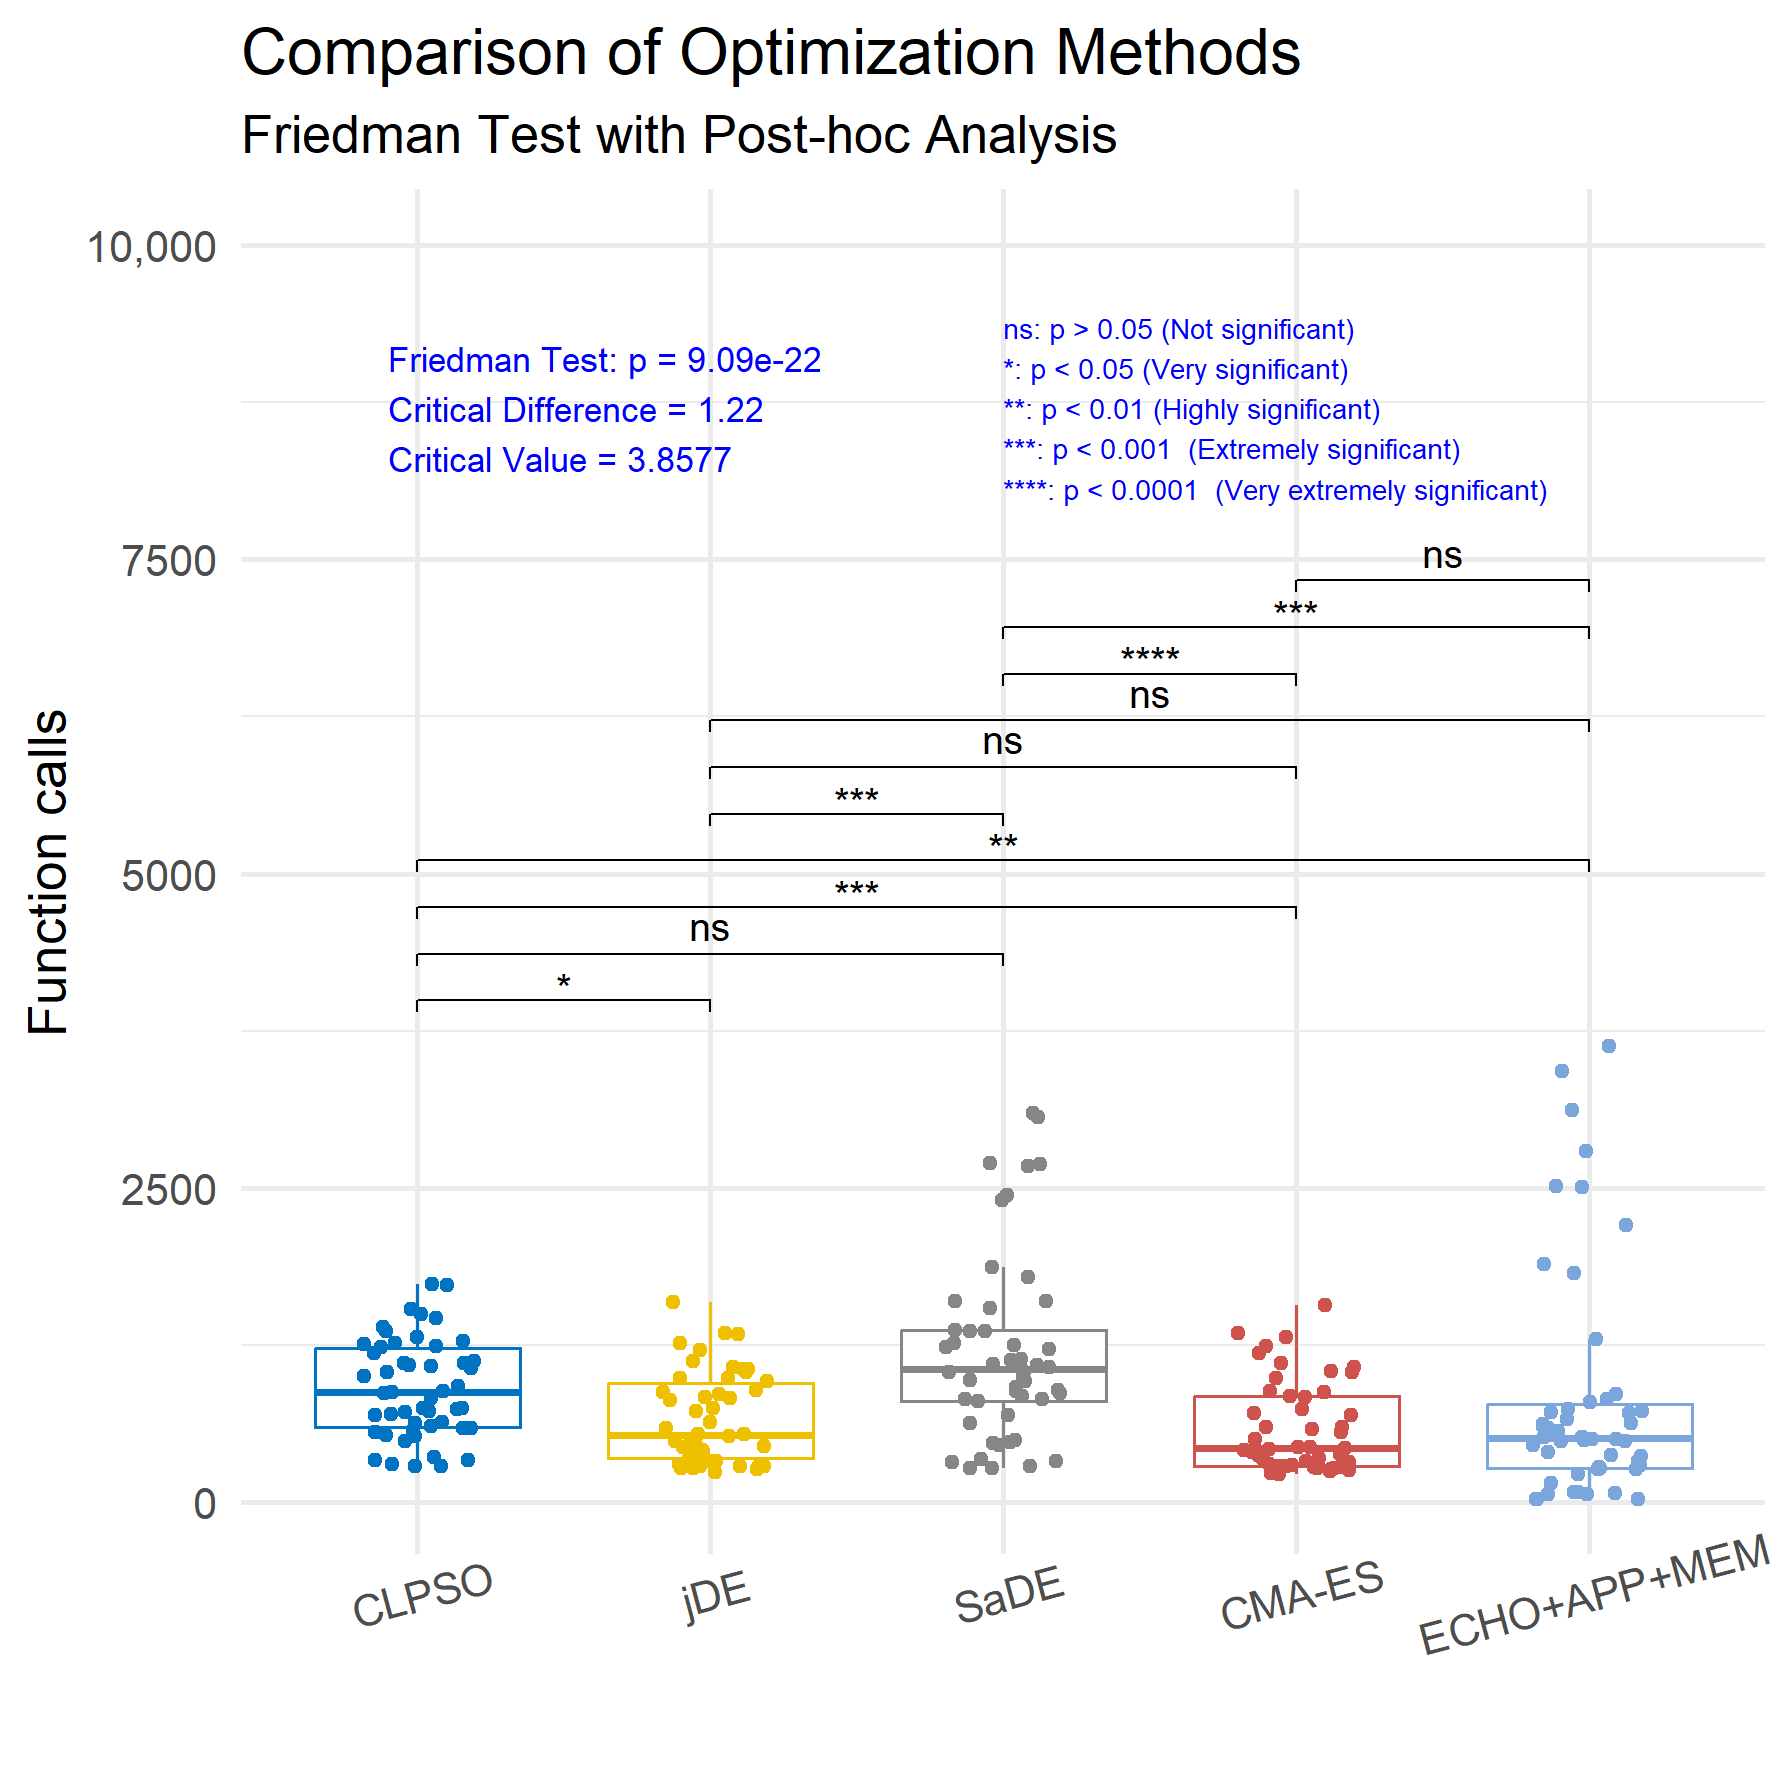
\includegraphics[scale=0.65]{poptype}
\par\end{centering}
\caption{Statistical comparison of function calls of the different optimization
methods for high-dimensional benchmark functions (population: formula)
\label{fig:statCallsPopFormula}}

\end{figure}

In Figure \ref{fig:statCallsPopFormula} the comparative analysis
between the ECHO+APP+MEM method and other well-known optimization
methods showed significant results based on the Friedman test, where
the p-value is extremely small (9.09e-22), indicating statistically
significant differences among the methods. The critical difference
is 1.22 and the critical value is 3.85. The ECHO+APP+MEM method demonstrated
statistically significant superiority compared to CLPSO (p\textless 0.01)
and SaDE (p\textless 0.001), while there were no statistically significant
differences compared to jDE and CMA-ES. Overall, the ECHO+APP+MEM
method appears to perform better or at least equivalently compared
to most of the methods tested, which reinforces its reliability and
effectiveness.

\begin{figure}[H]
\begin{centering}
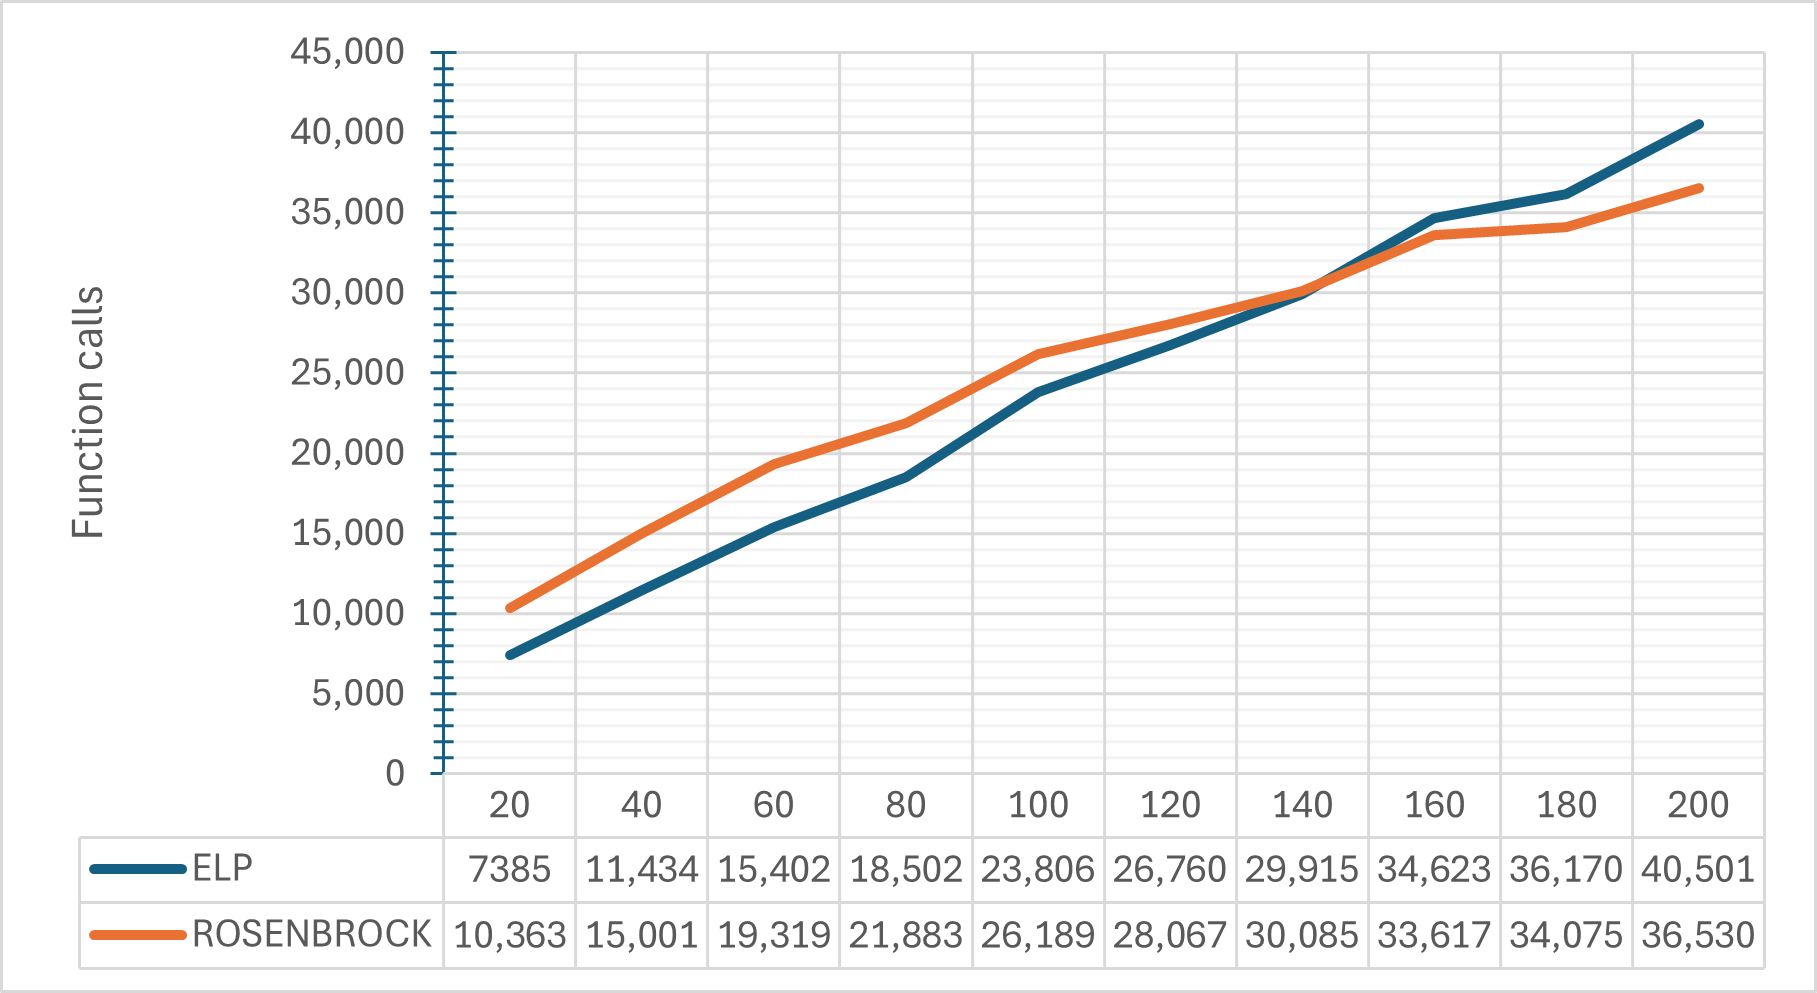
\includegraphics{callsMulti}
\par\end{centering}
\caption{Computational performance (Function calls) of the ECHO+APP+MEM method
on ELP and ROSENBROCK across dimensions 20-200 \label{fig:callsDim}}
\end{figure}

Figure \ref{fig:callsDim} illustrates the complexity of the ECHO+APP+MEM
method in relation to the problem dimensionality, which ranges from
20 to 200. The values represent the number of objective function calls
for the ELP and ROSENBROCK functions. It is observed that as dimensionality
increases, the number of function calls rises significantly for both
functions, indicating that the complexity of the method grows with
the problem size. For ELP, the calls increase from 7385 at dimension
20 to 40,501 at dimension 200, while for ROSENBROCK, the calls increase
from 10,363 to 36,530 respectively. This shows that the method requires
more computations for higher dimensions, which is expected for complex
optimization problems.

\begin{figure}[H]
\begin{centering}
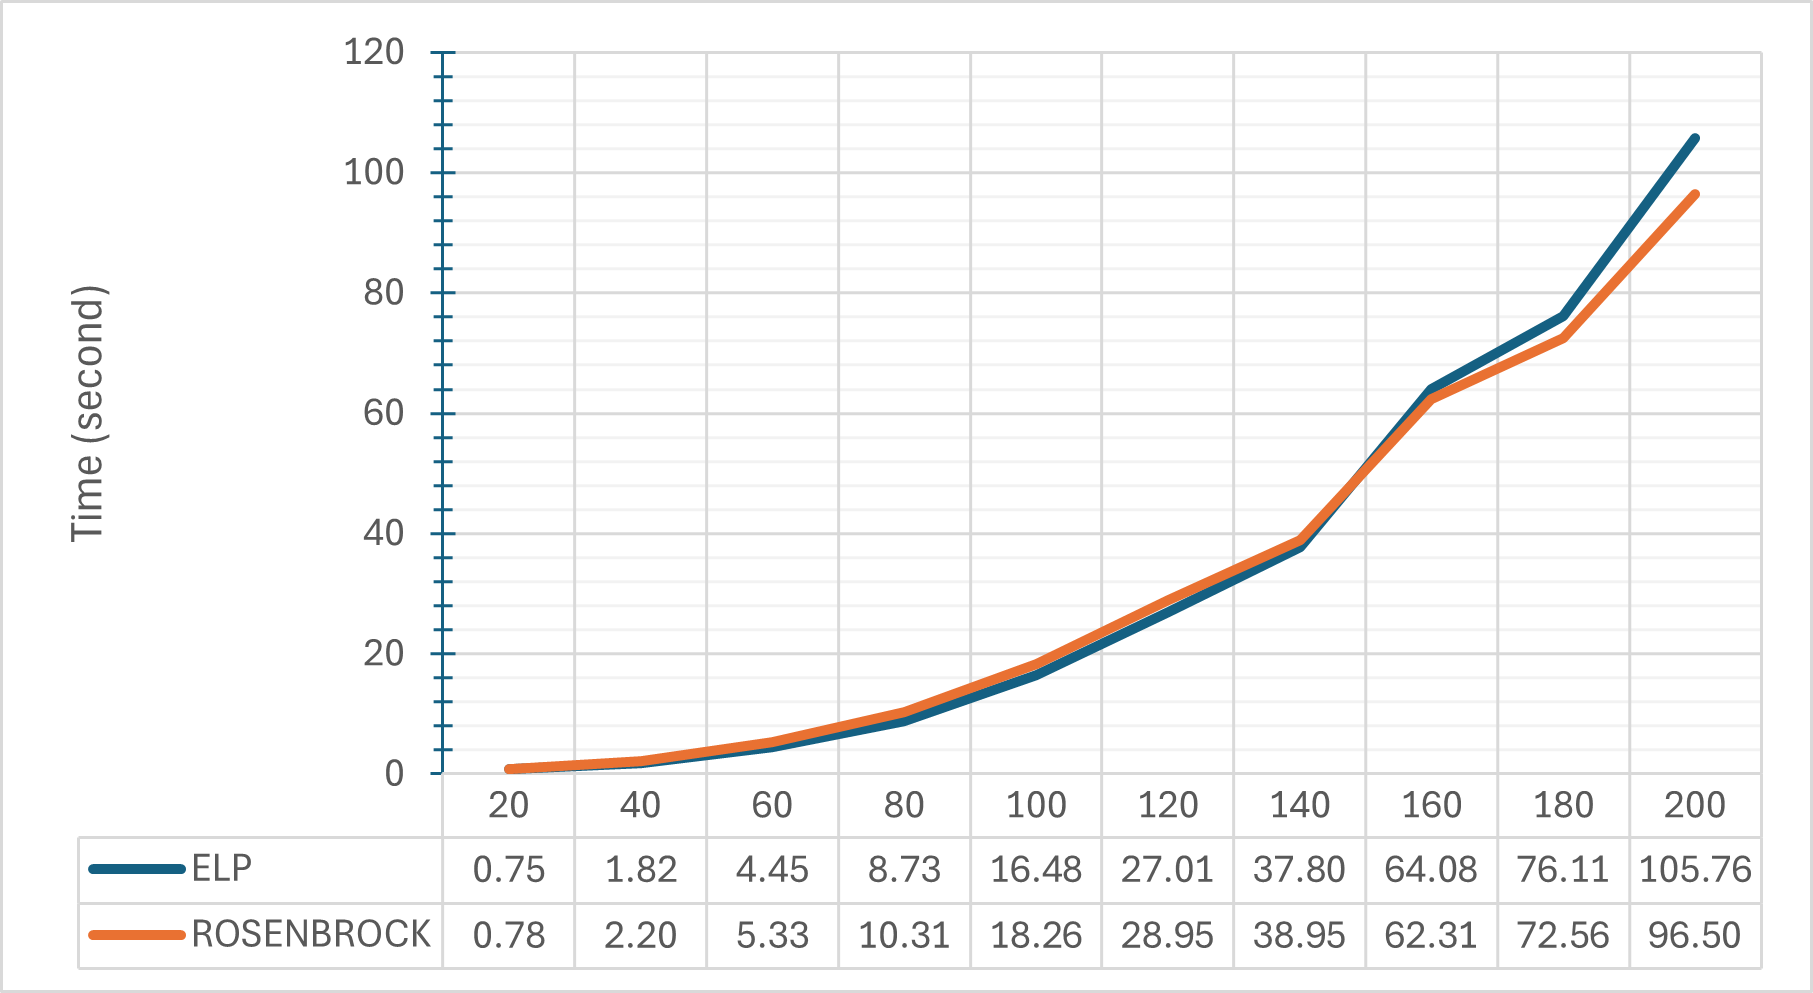
\includegraphics{timeMulti}
\par\end{centering}
\caption{Computational performance (Time) of the ECHO+APP+MEM method on ELP
and ROSENBROCK across dimensions 20-200 \label{fig:timesDim}}

\end{figure}

Figure \ref{fig:timesDim} shows the complexity of the ECHO+APP+MEM
method based on the solving time in seconds for the same functions
and dimensionalities. The solving time also increases with dimensionality,
starting from less than one second at dimension 20 and reaching approximately
106 seconds for ELP and 96.5 seconds for ROSENBROCK at dimension 200.
The increase in time is steady and corresponds to the increase in
the number of objective function calls, confirming that the method’s
complexity is linked to the dimensionality and the computational effort
required to solve the problems. Overall, both figures clearly show
that the ECHO+APP+MEM method remains functional and scalable but with
increasing computational cost as the problem dimension grows.

\subsection{Experiments on Real-World Problems}

In this section, experiments were conducted with a focus on real-world
optimization problems, selected from the set of functions listed in
Table \ref{tab:realProblems}, which represent approximately 85\%
of the entire CEC2011 benchmark set and encompass both classical and
contemporary challenges in global optimization. The experimental procedure
was carefully designed to ensure strict comparability among the different
algorithms under study. Specifically, a fixed population size of 100
samples, generated with a uniform distribution within the feasible
domain of each problem, was used for all methods except CMA-ES. For
CMA-ES, standard practice from the relevant literature was followed,
setting the population size according to the formula $Np=4+\left\lfloor 3\cdot\log(\text{dimension})\right\rfloor $
to optimally leverage the algorithm’s dynamics relative to problem
dimensionality. It is noteworthy that no local optimization phase
was applied in any experiment, thus allowing the pure global search
capability of each algorithm to be evaluated without the assistance
of local refinement procedures. All other parameters governing the
operation of the algorithms including evolution coefficients, stopping
rules, and acceptance criteriaremained unchanged and were set according
to the detailed configurations presented in Table 1, thereby ensuring
maximum objectivity in the comparative assessment of results. Through
this systematic approach, the experimental outcomes faithfully reflect
the behavior of the methods on demanding real-world problems, enabling
reliable conclusions to be drawn regarding their practical effectiveness.

The analysis of the results presented in Tables \ref{tab:algorithmsBestAndMean},
\ref{tab:rankingBestAndMean}, and \ref{tab:finalRanking} was based
on a rigorously standardized experimental protocol to ensure the reliability
and comparability of the methods. Specifically, for Table 9, the termination
criterion was strictly set to a fixed number of function evaluations
(1,500,000), providing all methods with equal opportunities for exploration
in the solution space. For each method, the best value (i.e., the
lowest objective function value found) and the mean value over 30
independent runs were recorded, thus capturing both the maximum and
average performance in a statistically substantiated manner. Subsequently,
in Table 10, the methods were ranked for each problem according to
their performance, with 1 corresponding to the best and 5 to the least
effective performance among the five methods. For drawing overall
conclusions, Table 11 presents the total sum of the ranks obtained
by each method for both the best and mean values, and this aggregate
score was divided by the total number of positions (i.e., the number
of methods multiplied by two, to account for both criteria), providing
a composite measure for comparing overall performance. Thus, the smallest
average total score indicates the most effective method, enabling
an objective evaluation of the comparative superiority of each approach
across the full set of problems.

{\tiny{}
\begin{table}[H]
{\footnotesize\caption{Real world problems CEC2011.\label{tab:realProblems}}
}{\footnotesize\par}
\centering{}{\tiny{}%
\begin{tabular}{|c|c|c|c|}
\hline 
{\tiny\textbf{PROBLEM}} & {\tiny\textbf{FORMULA}} & {\tiny\textbf{Dim}} & {\tiny\textbf{BOUNDS}}\tabularnewline
\hline 
\hline 
\begin{cellvarwidth}[t]
\centering
{\tiny\textbf{Parameter}}{\tiny\par}

{\tiny\textbf{Estimation for}}{\tiny\par}

{\tiny\textbf{Frequency-Modulated}}{\tiny\par}

{\tiny\textbf{Sound Waves}}
\end{cellvarwidth} & \begin{cellvarwidth}[t]
\centering
{\tiny$\min_{x\in[-6.4,6.35]^{6}}\;f(x)=\frac{1}{N}\sum_{n=1}^{N}\left|y(n;x)-y_{\text{target}}(n)\right|^{2}$}{\tiny\par}

{\tiny$y(n;x)=x_{0}\sin\left(x_{1}n+x_{2}\sin(x_{3}n+x_{4}\sin(x_{5}n))\right)$}
\end{cellvarwidth} & {\tiny 6} & {\tiny$x_{i}\in[-6.4,6.35]$}\tabularnewline
\hline 
\begin{cellvarwidth}[t]
\centering
{\tiny\textbf{Lennard-Jones}}{\tiny\par}

{\tiny\textbf{Potential}}
\end{cellvarwidth} & {\tiny$\min_{x\in\mathbb{R}^{3N-6}}\;f(x)=4\sum_{i=1}^{N-1}\sum_{j=i+1}^{N}\left[\left(\frac{1}{r_{ij}}\right)^{12}-\left(\frac{1}{r_{ij}}\right)^{6}\right]$} & {\tiny 30} & \begin{cellvarwidth}[t]
\centering
{\tiny$x_{0}\in(0,0,0)$}{\tiny\par}

{\tiny$x_{1},x_{2}\in[0,4]$}{\tiny\par}

{\tiny$x_{3}\in[0,\pi]$}{\tiny\par}

{\tiny$x_{3k-3}$}{\tiny\par}

{\tiny$x_{3k-2}$}{\tiny\par}

{\tiny$x_{i}\in[-b_{k},+b_{k}]$}
\end{cellvarwidth}\tabularnewline
\hline 
\begin{cellvarwidth}[t]
\centering
{\tiny\textbf{Bifunctional}}{\tiny\par}

{\tiny\textbf{Catalyst}}{\tiny\par}

{\tiny\textbf{Blend}}{\tiny\par}

{\tiny\textbf{Optimal}}{\tiny\par}

{\tiny\textbf{Control}}
\end{cellvarwidth} & \begin{cellvarwidth}[t]
\centering
{\tiny$\frac{dx_{1}}{dt}=-k_{1}x_{1}$, $\frac{dx_{2}}{dt}=k_{1}x_{1}-k_{2}x_{2}+k_{3}x_{2}+k_{4}x_{3}$,}{\tiny\par}

{\tiny$\frac{dx_{3}}{dt}=k_{2}x_{2}$, $\frac{dx_{4}}{dt}=-k_{4}x_{4}+k_{5}x_{5}$,}{\tiny\par}

{\tiny$\frac{dx_{5}}{dt}=-k_{3}x_{2}+k_{6}x_{4}-k_{5}x_{5}+k_{7}x_{6}+k_{8}x_{7}+k_{9}x_{5}+k_{10}x_{7}$}{\tiny\par}

{\tiny$\frac{dx_{6}}{dt}=k_{8}x_{5}-k_{7}x_{6}$, $\frac{dx_{7}}{dt}=k_{9}x_{5}-k_{10}x_{7}$}{\tiny\par}

{\tiny$k_{i}(u)=c_{i1}+c_{i2}u+c_{i3}u^{2}+c_{i4}u^{3}$}
\end{cellvarwidth} & {\tiny 1} & {\tiny$u\in[0.6,0.9]$}\tabularnewline
\hline 
\begin{cellvarwidth}[t]
\centering
{\tiny\textbf{Optimal}}{\tiny\par}

{\tiny\textbf{Control of a}}{\tiny\par}

{\tiny\textbf{Non-Linear}}{\tiny\par}

{\tiny\textbf{Stirred}}{\tiny\par}

{\tiny\textbf{Tank Reactor}}
\end{cellvarwidth} & \begin{cellvarwidth}[t]
\centering
{\tiny$J(u)=\int_{0}^{0.72}\left[x_{1}(t)^{2}+x_{2}(t)^{2}+0.1u^{2}\right]dt$}{\tiny\par}

{\tiny$\frac{dx_{1}}{dt}=-2x_{1}+x_{2}+1.25u+0.5\exp\left(\frac{x_{1}}{x_{1}+2}\right)$}{\tiny\par}

{\tiny$\frac{dx_{2}}{dt}=-x_{2}+0.5\exp\left(\frac{x_{1}}{x_{1}+2}\right)$}{\tiny\par}

{\tiny$x_{1}(0)=0.9,\quad x_{2}(0)=0.09$, $t\in[0,0.72]$}
\end{cellvarwidth} & {\tiny 1} & {\tiny$u\in[0,5]$}\tabularnewline
\hline 
\begin{cellvarwidth}[t]
\centering
{\tiny\textbf{Tersoff}}{\tiny\par}

{\tiny\textbf{Potential}}{\tiny\par}

{\tiny\textbf{for model Si (B)}}
\end{cellvarwidth} & \begin{cellvarwidth}[t]
\centering
{\tiny$\min_{\mathbf{x}\in\Omega}f(\mathbf{x})=\sum_{i=1}^{N}E(\mathbf{x}_{i})$}{\tiny\par}

{\tiny$E(\mathbf{x}_{i})=\frac{1}{2}\sum_{j\neq i}f_{c}(r_{ij})\left[V_{R}(r_{ij})-B_{ij}V_{A}(r_{ij})\right]$}{\tiny\par}

{\tiny where $r_{ij}=\|\mathbf{x}_{i}-\mathbf{x}_{j}\|$, $V_{R}(r)=A\exp(-\lambda_{1}r)$}{\tiny\par}

{\tiny$V_{A}(r)=B\exp(-\lambda_{2}r)$}{\tiny\par}

{\tiny$f_{c}(r)$: cutoff function with $f_{c}(r)$: angle parameter}
\end{cellvarwidth} & {\tiny 30} & \begin{cellvarwidth}[t]
\centering
{\tiny$x_{1}\in[0,4]$}{\tiny\par}

{\tiny$x_{2}\in[0,4]$}{\tiny\par}

{\tiny$x_{3}\in[0,\pi]$}{\tiny\par}

{\tiny$x_{i}\in\left[\frac{4(i-3)}{4},\ 4\right]$}
\end{cellvarwidth}\tabularnewline
\hline 
\begin{cellvarwidth}[t]
\centering
{\tiny\textbf{Tersoff}}{\tiny\par}

{\tiny\textbf{Potential}}{\tiny\par}

{\tiny\textbf{for model Si (C)}}
\end{cellvarwidth} & \begin{cellvarwidth}[t]
\centering
{\tiny$\min_{\mathbf{x}}\;V(\mathbf{x})=\sum_{i=1}^{N}\sum_{j>i}^{N}f_{C}(r_{ij})\left[a_{ij}f_{R}(r_{ij})+b_{ij}f_{A}(r_{ij})\right]$}{\tiny\par}

{\tiny$f_{C}(r)=\begin{cases}
1, & r<R-D\\
\frac{1}{2}+\frac{1}{2}\cos\left(\frac{\pi(r-R+D)}{2D}\right), & |r-R|\leq D\\
0, & r>R+D
\end{cases}$}{\tiny\par}

{\tiny$f_{R}(r)=A\exp(-\lambda_{1}r)$}{\tiny\par}

{\tiny$f_{A}(r)=-B\exp(-\lambda_{2}r)$}{\tiny\par}

{\tiny$b_{ij}=\left[1+(\beta^{n})\zeta_{ij}^{n}\right]^{-1/(2n)}$}{\tiny\par}

{\tiny$\sum_{k\neq i,j}f_{C}(r_{ik})g(\theta_{ijk})\exp\left[\lambda_{3}^{3}(r_{ij}-r_{ik})^{3}\right]$}
\end{cellvarwidth} & {\tiny 30} & \begin{cellvarwidth}[t]
\centering
{\tiny$x_{1}\in[0,4]$}{\tiny\par}

{\tiny$x_{2}\in[0,4]$}{\tiny\par}

{\tiny$x_{3}\in[0,\pi]$}{\tiny\par}

{\tiny$x_{i}\in\left[\frac{4(i-3)}{4},\ 4\right]$}
\end{cellvarwidth}\tabularnewline
\hline 
\begin{cellvarwidth}[t]
\centering
{\tiny\textbf{Spread}}{\tiny\par}

{\tiny\textbf{Spectrum Radar}}{\tiny\par}

{\tiny\textbf{Polly phase}}{\tiny\par}

{\tiny\textbf{Code Design}}
\end{cellvarwidth} & \begin{cellvarwidth}[t]
\centering
{\tiny$\min_{x\in X}\;f(x)=\max\left\{ |\varphi_{1}(x)|,|\varphi_{2}(x)|,\ldots,|\varphi_{m}(x)|\right\} $}{\tiny\par}

{\tiny$X=\{x\in\mathbb{R}^{n}\mid0\leq x_{j}\leq2\pi,\;j=1,\ldots,n\}m=2n-1$}{\tiny\par}

{\tiny$\varphi_{j}(x)=\begin{cases}
{\displaystyle \sum_{k=1}^{n-j}\cos(x_{k}-x_{k+j})} & \text{for }j=1,\ldots,n-1\\
{\displaystyle n} & \text{for }j=n\\
{\displaystyle \varphi_{2n-j}(x)} & \text{for }j=n+1,\ldots,2n-1
\end{cases}$}{\tiny\par}

{\tiny$\varphi_{j}(x)=\sum_{k=1}^{n-j}\cos(x_{k}-x_{k+j}),\quad j=1,\ldots,n-1$}{\tiny\par}

{\tiny$\varphi_{n}(x)=n$, $\varphi_{n+\ell}(x)=\varphi_{n-\ell}(x),\quad\ell=1,\ldots,n-1$}
\end{cellvarwidth} & {\tiny 20} & {\tiny$x_{j}\in[0,2\pi]$}\tabularnewline
\hline 
\begin{cellvarwidth}[t]
\centering
{\tiny\textbf{Transmission}}{\tiny\par}

{\tiny\textbf{Network}}{\tiny\par}

{\tiny\textbf{Expansion}}{\tiny\par}

{\tiny\textbf{Planning}}
\end{cellvarwidth} & \begin{cellvarwidth}[t]
\centering
{\tiny$\min\sum_{l\in\Omega}c_{l}n_{l}+W_{1}\sum_{l\in OL}|f_{l}-\bar{f}_{l}|+W_{2}\sum_{l\in\Omega}\max(0,n_{l}-\bar{n}_{l})$}{\tiny\par}

{\tiny$Sf=g-d$}{\tiny\par}

{\tiny$f_{l}=\gamma_{l}n_{l}\Delta\theta_{l},\quad\forall l\in\Omega$}{\tiny\par}

{\tiny$|f_{l}|\leq\bar{f}_{l}n_{l},\quad\forall l\in\Omega$}{\tiny\par}

{\tiny$0\leq n_{l}\leq\bar{n}_{l},\quad n_{l}\in\mathbb{Z},\quad\forall l\in\Omega$}
\end{cellvarwidth} & {\tiny 7} & \begin{cellvarwidth}[t]
\centering
{\tiny$0\leq n_{i}\leq\bar{n}_{l}$}{\tiny\par}

{\tiny$n_{i}\in\mathbb{Z}$}
\end{cellvarwidth}\tabularnewline
\hline 
\begin{cellvarwidth}[t]
\centering
{\tiny\textbf{Electricity}}{\tiny\par}

{\tiny\textbf{Transmission}}{\tiny\par}

{\tiny\textbf{Pricing}}
\end{cellvarwidth} & \begin{cellvarwidth}[t]
\centering
{\tiny$\min_{x}\;\;f(x)=\sum_{i=1}^{N_{g}}\left(\frac{C_{i}^{gen}}{P_{i}^{gen}}-R_{i}^{gen}\right)^{2}+\sum_{j=1}^{N_{d}}\left(\frac{C_{j}^{load}}{P_{j}^{load}}-R_{j}^{load}\right)^{2}$}{\tiny\par}

{\tiny$\sum_{j}GD_{i,j}+\sum_{j}BT_{i,j}=P_{i}^{gen},\quad\forall i$}{\tiny\par}

{\tiny$\sum_{i}GD_{i,j}+\sum_{i}BT_{i,j}=P_{j}^{load},\quad\forall j$}{\tiny\par}

{\tiny$GD_{i,j}^{max}=\min(P_{i}^{gen}-BT_{i,j},\;P_{j}^{load}-BT_{i,j})$}
\end{cellvarwidth} & {\tiny 126} & {\tiny$GD_{i,j}\in[0,GD_{i,j}^{max}]$}\tabularnewline
\hline 
\begin{cellvarwidth}[t]
\centering
{\tiny\textbf{Circular}}{\tiny\par}

{\tiny\textbf{Antenna}}{\tiny\par}

{\tiny\textbf{Array}}{\tiny\par}

{\tiny\textbf{Design}}
\end{cellvarwidth} & \begin{cellvarwidth}[t]
\centering
{\tiny$\min_{r_{1},\ldots,r_{6},\,\varphi_{1},\ldots,\varphi_{6}}\quad f(\mathbf{x})=\max_{\theta\in\Omega}AF(\mathbf{x},\theta)$}{\tiny\par}

{\tiny$AF(\mathbf{x},\theta)=\left|\sum_{k=1}^{6}\exp\left(j\left[2\pi r_{k}\cos(\theta-\theta_{k})+\varphi_{k}\frac{\pi}{180}\right]\right)\right|$}
\end{cellvarwidth} & {\tiny 12} & \begin{cellvarwidth}[t]
\centering
{\tiny$r_{k}\in[0.2,1]$}{\tiny\par}

{\tiny$\varphi_{k}\in[-180,180]$}
\end{cellvarwidth}\tabularnewline
\hline 
\begin{cellvarwidth}[t]
\centering
{\tiny\textbf{Dynamic}}{\tiny\par}

{\tiny\textbf{Economic}}{\tiny\par}

{\tiny\textbf{Dispatch 1}}
\end{cellvarwidth} & \begin{cellvarwidth}[t]
\centering
{\tiny$\min_{\mathbf{P}}\quad f(\mathbf{P})=\sum_{t=1}^{24}\sum_{i=1}^{5}\left(a_{i}P_{i,t}^{2}+b_{i}P_{i,t}+c_{i}\right)$}{\tiny\par}

{\tiny$P_{i}^{\min}\leq P_{i,t}\leq P_{i}^{\max},\quad\forall i=1,\ldots,5,\;t=1,\ldots,24$}{\tiny\par}

{\tiny$\sum_{i=1}^{5}P_{i,t}=D_{t},\quad\forall t=1,\ldots,24$}{\tiny\par}

{\tiny$P_{\min}=[10,20,30,40,50]$}{\tiny\par}

{\tiny$P_{\max}=[75,125,175,250,300]$}
\end{cellvarwidth} & {\tiny 120} & {\tiny$P_{i}^{\min}\leq P_{i,t}\leq P_{i}^{\max}$}\tabularnewline
\hline 
\begin{cellvarwidth}[t]
\centering
{\tiny\textbf{Dynamic}}{\tiny\par}

{\tiny\textbf{Economic}}{\tiny\par}

{\tiny\textbf{Dispatch 2}}
\end{cellvarwidth} & \begin{cellvarwidth}[t]
\centering
{\tiny$\min_{\mathbf{P}}\quad f(\mathbf{P})=\sum_{t=1}^{24}\sum_{i=1}^{9}\left(a_{i}P_{i,t}^{2}+b_{i}P_{i,t}+c_{i}\right)$}{\tiny\par}

{\tiny$P_{i}^{\min}\leq P_{i,t}\leq P_{i}^{\max},\quad\forall i=1,\ldots,5,\;t=1,\ldots,24$}{\tiny\par}

{\tiny$\sum_{i=1}^{5}P_{i,t}=D_{t},\quad\forall t=1,\ldots,24$}{\tiny\par}

{\tiny$P_{\min}=[150,135,73,60,73,57,20,47,20]$}{\tiny\par}

{\tiny$P_{\max}=[470,460,340,300,243,160,130,120,80]$}
\end{cellvarwidth} & {\tiny 216} & {\tiny$P_{i}^{\min}\leq P_{i,t}\leq P_{i}^{\max}$}\tabularnewline
\hline 
\begin{cellvarwidth}[t]
\centering
{\tiny\textbf{Static}}{\tiny\par}

{\tiny\textbf{Economic}}{\tiny\par}

{\tiny\textbf{Load}}{\tiny\par}

{\tiny\textbf{Dispatch}}{\tiny\par}

{\tiny\textbf{(1,2,3,4,5)}}
\end{cellvarwidth} & \begin{cellvarwidth}[t]
\centering
{\tiny$\min_{P_{1},\ldots,P_{N_{G}}}F=\sum_{i=1}^{N_{G}}f_{i}(P_{i})$}{\tiny\par}

{\tiny$f_{i}(P_{i})=a_{i}P_{i}^{2}+b_{i}P_{i}+c_{i},\quad i=1,2,\ldots,N_{G}$}{\tiny\par}

{\tiny$f_{i}(P_{i})=a_{i}P_{i}^{2}+b_{i}P_{i}+c_{i}+|e_{i}\sin(f_{i}(P_{i}^{\min}-P_{i}))|$}{\tiny\par}

{\tiny$P_{i}^{\min}\leq P_{i}\leq P_{i}^{\max},\quad i=1,2,\ldots,N_{G}$}{\tiny\par}

{\tiny$\sum_{i=1}^{N_{G}}P_{i}=P_{D}+P_{L}$}{\tiny\par}

{\tiny$P_{L}=\sum_{i=1}^{N_{G}}\sum_{j=1}^{N_{G}}P_{i}B_{ij}P_{j}+\sum_{i=1}^{N_{G}}B_{0i}P_{i}+B_{00}$}{\tiny\par}

{\tiny$P_{i}-P_{i}^{0}\leq UR_{i}\quad P_{i}^{0}-P_{i}\leq DR_{i}$}
\end{cellvarwidth} & \begin{cellvarwidth}[t]
\centering
{\tiny 6}{\tiny\par}

{\tiny 13}{\tiny\par}

{\tiny 15}{\tiny\par}

{\tiny 40}{\tiny\par}

{\tiny 140}
\end{cellvarwidth} & \begin{cellvarwidth}[t]
\centering
{\tiny See}{\tiny\par}

{\tiny Technical}{\tiny\par}

{\tiny Report}{\tiny\par}

{\tiny of}{\tiny\par}

{\tiny CEC2011}
\end{cellvarwidth}\tabularnewline
\hline 
\end{tabular}}{\tiny\par}
\end{table}
}{\tiny{}
\begin{sidewaystable}[H]
{\footnotesize\caption{Algorithms’ Comparison Based on Best and Mean after 1.5e+5 FEs.+\label{tab:algorithmsBestAndMean}}
}{\footnotesize\par}
\centering{}{\scriptsize{}%
\begin{tabular}{|V{\linewidth}|c|c|c|c|c|c|c|c|c|c|}
\hline 
{\scriptsize\textbf{PROBLEM}} & \begin{cellvarwidth}[t]
\centering
{\scriptsize\textbf{CLPSO}}{\scriptsize\par}

{\scriptsize\textbf{best}}
\end{cellvarwidth} & \begin{cellvarwidth}[t]
\centering
{\scriptsize\textbf{CLPSO}}{\scriptsize\par}

{\scriptsize\textbf{Mean}}
\end{cellvarwidth} & \begin{cellvarwidth}[t]
\centering
{\scriptsize\textbf{SaDE}}{\scriptsize\par}

{\scriptsize\textbf{best}}
\end{cellvarwidth} & \begin{cellvarwidth}[t]
\centering
{\scriptsize\textbf{SaDE}}{\scriptsize\par}

{\scriptsize\textbf{Mean}}
\end{cellvarwidth} & \begin{cellvarwidth}[t]
\centering
{\scriptsize\textbf{jDE}}{\scriptsize\par}

{\scriptsize\textbf{Best}}
\end{cellvarwidth} & \begin{cellvarwidth}[t]
\centering
{\scriptsize\textbf{jDE}}{\scriptsize\par}

{\scriptsize\textbf{Mean}}
\end{cellvarwidth} & \begin{cellvarwidth}[t]
\centering
{\scriptsize\textbf{CMA-ES}}{\scriptsize\par}

{\scriptsize\textbf{best}}
\end{cellvarwidth} & \begin{cellvarwidth}[t]
\centering
{\scriptsize\textbf{CMA-ES}}{\scriptsize\par}

{\scriptsize\textbf{Mean}}
\end{cellvarwidth} & \begin{cellvarwidth}[t]
\centering
{\scriptsize\textbf{EO}}{\scriptsize\par}

{\scriptsize\textbf{Best}}
\end{cellvarwidth} & \begin{cellvarwidth}[t]
\centering
{\scriptsize\textbf{EO}}{\scriptsize\par}

{\scriptsize\textbf{Mean}}
\end{cellvarwidth}\tabularnewline
\hline 
\hline 
{\scriptsize\textbf{Parameter Estimation for}}{\scriptsize\par}

{\scriptsize\textbf{Frequency-Modulated Sound Waves}} & {\scriptsize 0.1314837477} & {\scriptsize 0.2124981688} & {\scriptsize 0.1899428536} & {\scriptsize 0.2025566839} & {\scriptsize 0.2915779318} & {\scriptsize 0.372177177} & {\scriptsize 0.18160916} & {\scriptsize 0.256863966} & {\scriptsize 0.2521750203} & {\scriptsize 0.2954215036}\tabularnewline
\hline 
{\scriptsize\textbf{Lennard-Jones}}{\scriptsize\par}

{\scriptsize\textbf{Potential}} & {\scriptsize -13.43649135} & {\scriptsize -10.25073403} & {\scriptsize -24.86870825} & {\scriptsize -22.6693403} & {\scriptsize -26.96868295} & {\scriptsize -23.05977012} & {\scriptsize -28.42253189} & {\scriptsize -25.78783328} & {\scriptsize -15.93299933} & {\scriptsize -12.14897801}\tabularnewline
\hline 
{\scriptsize\textbf{BifunctionalCatalyst Blend}}{\scriptsize\par}

{\scriptsize\textbf{Optimal Control}} & {\scriptsize 0.2374871493} & {\scriptsize 0.4314871688} & {\scriptsize 0.545953325} & {\scriptsize 0.624508763} & {\scriptsize 0.545624975} & {\scriptsize 0.6003624983} & {\scriptsize 0.1314837477} & {\scriptsize 0.2445629767} & {\scriptsize 0.245874592} & {\scriptsize 0.3935178477}\tabularnewline
\hline 
{\scriptsize\textbf{Optimal Control of a Non-}}{\scriptsize\par}

{\scriptsize\textbf{Linear Stirred Tank Reactor}} & {\scriptsize 0.3903767228} & {\scriptsize 0.3903767228} & {\scriptsize 0.3903767228} & {\scriptsize 0.3903767228} & {\scriptsize 0.4913066735} & {\scriptsize 7.309621249e+10} & {\scriptsize 0.3903767228} & {\scriptsize 0.390376723} & {\scriptsize 38.94304848} & {\scriptsize 26682.93618}\tabularnewline
\hline 
{\scriptsize\textbf{Tersoff Potential}}{\scriptsize\par}

{\scriptsize\textbf{for model Si (B)}} & {\scriptsize -28.23544117} & {\scriptsize -26.18834522} & {\scriptsize -3.107773136} & {\scriptsize 25.4711091} & {\scriptsize -22.10581388} & {\scriptsize -2.387797305} & {\scriptsize -29.26244222} & {\scriptsize -27.5889735} & {\scriptsize -26.7539495} & {\scriptsize -24.83294286}\tabularnewline
\hline 
{\scriptsize\textbf{Tersoff Potential}}{\scriptsize\par}

{\scriptsize\textbf{for model Si (C)}} & {\scriptsize -30.85200257} & {\scriptsize -28.87349048} & {\scriptsize -11.60719468} & {\scriptsize 22.08963599} & {\scriptsize -23.1614585} & {\scriptsize -7.886665429} & {\scriptsize -33.19699356} & {\scriptsize -31.79270914} & {\scriptsize -31.49334757} & {\scriptsize -28.7003262}\tabularnewline
\hline 
{\scriptsize\textbf{Spread Spectrum Radar}}{\scriptsize\par}

{\scriptsize\textbf{Polly phaseCode Design}} & {\scriptsize 1.085334991} & {\scriptsize 1.343956153} & {\scriptsize 1.536501579} & {\scriptsize 2.150881715} & {\scriptsize 0.9189283507} & {\scriptsize 1.616525419} & {\scriptsize 0.014848227} & {\scriptsize 0.171988666} & {\scriptsize 0.5931349058} & {\scriptsize 0.8611681213}\tabularnewline
\hline 
{\scriptsize\textbf{Transmission Network}}{\scriptsize\par}

{\scriptsize\textbf{Expansion Planning}} & {\scriptsize 250} & {\scriptsize 250} & {\scriptsize 250} & {\scriptsize 250} & {\scriptsize 250} & {\scriptsize 250} & {\scriptsize 250} & {\scriptsize 250} & {\scriptsize 250} & {\scriptsize 250}\tabularnewline
\hline 
{\scriptsize\textbf{Electricity Transmission}}{\scriptsize\par}

{\scriptsize\textbf{Pricing}} & {\scriptsize 13775010.1} & {\scriptsize 13775395.07} & {\scriptsize 23481009.86} & {\scriptsize 30034934.81} & {\scriptsize 13776257.77} & {\scriptsize 14484728.07} & {\scriptsize 13775841.77} & {\scriptsize 13787550.18} & {\scriptsize 13776506.06} & {\scriptsize 13777507.07}\tabularnewline
\hline 
{\scriptsize\textbf{Circular Antenna}}{\scriptsize\par}

{\scriptsize\textbf{Array Design}} & {\scriptsize 0.006933401045} & {\scriptsize 0.05181551798} & {\scriptsize 0.02142329927} & {\scriptsize 0.03892428051} & {\scriptsize 0.04238306654} & {\scriptsize 0.1610286721} & {\scriptsize 0.007204797576} & {\scriptsize 0.008635655364} & {\scriptsize 0.03477651401} & {\scriptsize 0.1675322066}\tabularnewline
\hline 
{\scriptsize\textbf{Dynamic Economic}}{\scriptsize\par}

{\scriptsize\textbf{Dispatch 1}} & {\scriptsize 428607927.6} & {\scriptsize 435250914.5} & {\scriptsize 968042312.1} & {\scriptsize 1034679775} & {\scriptsize 968042312.1} & {\scriptsize 1071143842} & {\scriptsize 88285.6024} & {\scriptsize 102776.7103} & {\scriptsize 473972051.7} & {\scriptsize 496720571.7}\tabularnewline
\hline 
{\scriptsize\textbf{Dynamic Economic}}{\scriptsize\par}

{\scriptsize\textbf{Dispatch 2}} & {\scriptsize 33031590.31} & {\scriptsize 53906147.38} & {\scriptsize 845287898.3} & {\scriptsize 913715793.2} & {\scriptsize 350885523} & {\scriptsize 456293948.4} & {\scriptsize 502699.4187} & {\scriptsize 477720.1511} & {\scriptsize 77187145.39} & {\scriptsize 92911983.83}\tabularnewline
\hline 
{\scriptsize\textbf{Static Economic}}{\scriptsize\par}

{\scriptsize\textbf{Load Dispatch 1}} & {\scriptsize 6554.672173} & {\scriptsize 7668.333603} & {\scriptsize 16877.92071} & {\scriptsize 101588.3887} & {\scriptsize 6473.96039} & {\scriptsize 939805.3726} & {\scriptsize 6657.613028} & {\scriptsize 415917.4625} & {\scriptsize 6878.581584} & {\scriptsize 12522.32104}\tabularnewline
\hline 
{\scriptsize\textbf{Static Economic}}{\scriptsize\par}

{\scriptsize\textbf{Load Dispatch 2}} & {\scriptsize 19030.36081} & {\scriptsize 20699.00219} & {\scriptsize 2600565.214} & {\scriptsize 9329466.813} & {\scriptsize 41350.66254} & {\scriptsize 8649652.933} & {\scriptsize 763001.2185} & {\scriptsize 1425815.44} & {\scriptsize 19406.19272} & {\scriptsize 44368.22458}\tabularnewline
\hline 
{\scriptsize\textbf{Static Economic}}{\scriptsize\par}

{\scriptsize\textbf{Load Dispatch 3}} & {\scriptsize 470192288.3} & {\scriptsize 470294703.2} & {\scriptsize 478069615.3} & {\scriptsize 541898763} & {\scriptsize 474743051.8} & {\scriptsize 514454706.1} & {\scriptsize 470023232.3} & {\scriptsize 470023232.3} & {\scriptsize 470437730.6} & {\scriptsize 470713100.1}\tabularnewline
\hline 
{\scriptsize\textbf{Static Economic}}{\scriptsize\par}

{\scriptsize\textbf{Load Dispatch 4}} & {\scriptsize 884980.5569} & {\scriptsize 1423887.358} & {\scriptsize 14170362.58} & {\scriptsize 106749078.5} & {\scriptsize 14657102.04} & {\scriptsize 32906828.34} & {\scriptsize 476053.5197} & {\scriptsize 2925852.935} & {\scriptsize 149544.9615} & {\scriptsize 417426.7844}\tabularnewline
\hline 
{\scriptsize\textbf{Static Economic}}{\scriptsize\par}

{\scriptsize\textbf{Load Dispatch 5}} & {\scriptsize 8105947615} & {\scriptsize 8110924071} & {\scriptsize 8901002004} & {\scriptsize 9943082701} & {\scriptsize 8446155955} & {\scriptsize 463055675} & {\scriptsize 8072077963} & {\scriptsize 8084017791} & {\scriptsize 8119017656} & {\scriptsize 8263919973}\tabularnewline
\hline 
\end{tabular}}{\scriptsize\par}
\end{sidewaystable}
}
\begin{sidewaystable}[H]
\caption{Algorithms’ Comparison Based on Best and Mean after 1.5e+5 FEs.\label{tab:rankingBestAndMean}}

\centering{}{\footnotesize{}%
\begin{tabular}{|V{\linewidth}|c|c|c|c|c|c|c|c|c|c|}
\hline 
{\footnotesize\textbf{PROBLEM}} & \begin{cellvarwidth}[t]
\centering
{\footnotesize\textbf{CLPSO}}{\footnotesize\par}

{\footnotesize\textbf{best}}
\end{cellvarwidth} & \begin{cellvarwidth}[t]
\centering
{\footnotesize\textbf{CLPSO}}{\footnotesize\par}

{\footnotesize\textbf{Mean}}
\end{cellvarwidth} & \begin{cellvarwidth}[t]
\centering
{\footnotesize\textbf{SaDE}}{\footnotesize\par}

{\footnotesize\textbf{best}}
\end{cellvarwidth} & \begin{cellvarwidth}[t]
\centering
{\footnotesize\textbf{SaDE}}{\footnotesize\par}

{\footnotesize\textbf{Mean}}
\end{cellvarwidth} & \begin{cellvarwidth}[t]
\centering
{\footnotesize\textbf{jDE}}{\footnotesize\par}

{\footnotesize\textbf{Best}}
\end{cellvarwidth} & \begin{cellvarwidth}[t]
\centering
{\footnotesize\textbf{jDE}}{\footnotesize\par}

{\footnotesize\textbf{Mean}}
\end{cellvarwidth} & \begin{cellvarwidth}[t]
\centering
{\footnotesize\textbf{CMA-ES}}{\footnotesize\par}

{\footnotesize\textbf{best}}
\end{cellvarwidth} & \begin{cellvarwidth}[t]
\centering
{\footnotesize\textbf{CMA-ES}}{\footnotesize\par}

{\footnotesize\textbf{Mean}}
\end{cellvarwidth} & \begin{cellvarwidth}[t]
\centering
{\footnotesize\textbf{EO}}{\footnotesize\par}

{\footnotesize\textbf{Best}}
\end{cellvarwidth} & \begin{cellvarwidth}[t]
\centering
{\footnotesize\textbf{EO}}{\footnotesize\par}

{\footnotesize\textbf{Mean}}
\end{cellvarwidth}\tabularnewline
\hline 
\hline 
{\footnotesize\textbf{Parameter Estimation for}}{\footnotesize\par}

{\footnotesize\textbf{Frequency-Modulated Sound Waves}} & {\footnotesize 1} & {\footnotesize 2} & {\footnotesize 3} & {\footnotesize 1} & {\footnotesize 5} & {\footnotesize 5} & {\footnotesize 2} & {\footnotesize 3} & {\footnotesize 4} & {\footnotesize 4}\tabularnewline
\hline 
{\footnotesize\textbf{Lennard-Jones}}{\footnotesize\par}

{\footnotesize\textbf{Potential}} & {\footnotesize 5} & {\footnotesize 5} & {\footnotesize 3} & {\footnotesize 3} & {\footnotesize 2} & {\footnotesize 2} & {\footnotesize 1} & {\footnotesize 1} & {\footnotesize 4} & {\footnotesize 4}\tabularnewline
\hline 
{\footnotesize\textbf{BifunctionalCatalyst Blend}}{\footnotesize\par}

{\footnotesize\textbf{Optimal Control}} & {\footnotesize 2} & {\footnotesize 2} & {\footnotesize 5} & {\footnotesize 5} & {\footnotesize 4} & {\footnotesize 4} & {\footnotesize 1} & {\footnotesize 1} & {\footnotesize 3} & {\footnotesize 3}\tabularnewline
\hline 
{\footnotesize\textbf{Optimal Control of a}}{\footnotesize\par}

{\footnotesize\textbf{Non-Linear Stirred}}{\footnotesize\par}

{\footnotesize\textbf{Tank Reactor}} & {\footnotesize 1} & {\footnotesize 1} & {\footnotesize 1} & {\footnotesize 1} & {\footnotesize 3} & {\footnotesize 3} & {\footnotesize 1} & {\footnotesize 1} & {\footnotesize 4} & {\footnotesize 4}\tabularnewline
\hline 
{\footnotesize\textbf{Tersoff Potential}}{\footnotesize\par}

{\footnotesize\textbf{for model Si (B)}} & {\footnotesize 2} & {\footnotesize 2} & {\footnotesize 5} & {\footnotesize 5} & {\footnotesize 4} & {\footnotesize 4} & {\footnotesize 1} & {\footnotesize 1} & {\footnotesize 3} & {\footnotesize 3}\tabularnewline
\hline 
{\footnotesize\textbf{Tersoff Potential}}{\footnotesize\par}

{\footnotesize\textbf{for model Si (C)}} & {\footnotesize 2} & {\footnotesize 2} & {\footnotesize 5} & {\footnotesize 5} & {\footnotesize 4} & {\footnotesize 4} & {\footnotesize 1} & {\footnotesize 1} & {\footnotesize 3} & {\footnotesize 3}\tabularnewline
\hline 
{\footnotesize\textbf{Spread Spectrum Radar}}{\footnotesize\par}

{\footnotesize\textbf{Polly phaseCode Design}} & {\footnotesize 4} & {\footnotesize 3} & {\footnotesize 5} & {\footnotesize 5} & {\footnotesize 3} & {\footnotesize 4} & {\footnotesize 1} & {\footnotesize 1} & {\footnotesize 2} & {\footnotesize 2}\tabularnewline
\hline 
{\footnotesize\textbf{Transmission Network}}{\footnotesize\par}

{\footnotesize\textbf{Expansion Planning}} & {\footnotesize 1} & {\footnotesize 1} & {\footnotesize 1} & {\footnotesize 1} & {\footnotesize 1} & {\footnotesize 1} & {\footnotesize 1} & {\footnotesize 1} & {\footnotesize 1} & {\footnotesize 1}\tabularnewline
\hline 
{\footnotesize\textbf{Electricity Transmission}}{\footnotesize\par}

{\footnotesize\textbf{Pricing}} & {\footnotesize 2} & {\footnotesize 1} & {\footnotesize 5} & {\footnotesize 5} & {\footnotesize 1} & {\footnotesize 4} & {\footnotesize 3} & {\footnotesize 3} & {\footnotesize 4} & {\footnotesize 2}\tabularnewline
\hline 
{\footnotesize\textbf{Circular Antenna}}{\footnotesize\par}

{\footnotesize\textbf{Array Design}} & {\footnotesize 1} & {\footnotesize 3} & {\footnotesize 3} & {\footnotesize 2} & {\footnotesize 5} & {\footnotesize 4} & {\footnotesize 2} & {\footnotesize 1} & {\footnotesize 4} & {\footnotesize 5}\tabularnewline
\hline 
{\footnotesize\textbf{Dynamic Economic}}{\footnotesize\par}

{\footnotesize\textbf{Dispatch 1}} & {\footnotesize 2} & {\footnotesize 2} & {\footnotesize 4} & {\footnotesize 4} & {\footnotesize 4} & {\footnotesize 5} & {\footnotesize 1} & {\footnotesize 1} & {\footnotesize 3} & {\footnotesize 3}\tabularnewline
\hline 
{\footnotesize\textbf{Dynamic Economic}}{\footnotesize\par}

{\footnotesize\textbf{Dispatch 2}} & {\footnotesize 2} & {\footnotesize 2} & {\footnotesize 5} & {\footnotesize 5} & {\footnotesize 4} & {\footnotesize 4} & {\footnotesize 1} & {\footnotesize 1} & {\footnotesize 3} & {\footnotesize 3}\tabularnewline
\hline 
{\footnotesize\textbf{Static Economic}}{\footnotesize\par}

{\footnotesize\textbf{Load Dispatch 1}} & {\footnotesize 2} & {\footnotesize 1} & {\footnotesize 5} & {\footnotesize 3} & {\footnotesize 1} & {\footnotesize 5} & {\footnotesize 3} & {\footnotesize 4} & {\footnotesize 4} & {\footnotesize 2}\tabularnewline
\hline 
{\footnotesize\textbf{Static Economic}}{\footnotesize\par}

{\footnotesize\textbf{Load Dispatch 2}} & {\footnotesize 1} & {\footnotesize 1} & {\footnotesize 3} & {\footnotesize 5} & {\footnotesize 4} & {\footnotesize 4} & {\footnotesize 5} & {\footnotesize 3} & {\footnotesize 2} & {\footnotesize 2}\tabularnewline
\hline 
{\footnotesize\textbf{Static Economic}}{\footnotesize\par}

{\footnotesize\textbf{Load Dispatch 3}} & {\footnotesize 2} & {\footnotesize 2} & {\footnotesize 5} & {\footnotesize 5} & {\footnotesize 4} & {\footnotesize 4} & {\footnotesize 1} & {\footnotesize 1} & {\footnotesize 3} & {\footnotesize 3}\tabularnewline
\hline 
{\footnotesize\textbf{Static Economic}}{\footnotesize\par}

{\footnotesize\textbf{Load Dispatch 4}} & {\footnotesize 3} & {\footnotesize 2} & {\footnotesize 4} & {\footnotesize 5} & {\footnotesize 5} & {\footnotesize 4} & {\footnotesize 2} & {\footnotesize 3} & {\footnotesize 1} & {\footnotesize 1}\tabularnewline
\hline 
{\footnotesize\textbf{Static Economic}}{\footnotesize\par}

{\footnotesize\textbf{Load Dispatch 5}} & {\footnotesize 2} & {\footnotesize 2} & {\footnotesize 5} & {\footnotesize 5} & {\footnotesize 4} & {\footnotesize 4} & {\footnotesize 1} & {\footnotesize 1} & {\footnotesize 3} & {\footnotesize 3}\tabularnewline
\hline 
{\footnotesize\textbf{TOTAL}} & {\footnotesize\textbf{35}} & {\footnotesize\textbf{34}} & {\footnotesize\textbf{68}} & {\footnotesize\textbf{66}} & {\footnotesize 60} & {\footnotesize 68} & {\footnotesize\textbf{28}} & {\footnotesize\textbf{28}} & {\footnotesize\textbf{54}} & {\footnotesize 51}\tabularnewline
\hline 
\end{tabular}}{\footnotesize\par}
\end{sidewaystable}
\begin{table}[H]
\caption{Comparison of algorithms and final ranking\label{tab:finalRanking}}

\begin{centering}
\begin{tabular}{|c|c|c|c|c|c|}
\hline 
\textbf{Problem} & \textbf{Best} & \textbf{Mean} & \textbf{Overall} & \textbf{Average} & \textbf{Rang}\tabularnewline
\hline 
\hline 
\textbf{CMA-ES} & 28 & 28 & 56 & 1.647 & \textbf{1}\tabularnewline
\hline 
\textbf{CLPSO} & 35 & 34 & 69 & 2.029 & \textbf{2}\tabularnewline
\hline 
\textbf{EO} & 51 & 48 & 99 & 2.9116 & \textbf{3}\tabularnewline
\hline 
\textbf{jDE} & 58 & 65 & 123 & 3.617 & \textbf{4}\tabularnewline
\hline 
\textbf{SaDE} & 67 & 65 & 132 & 3.882 & \textbf{5}\tabularnewline
\hline 
\end{tabular}
\par\end{centering}
\end{table}

In the comparative assessment conducted in this subsection, the basic
form of the EO was benchmarked against other modern and internationally
recognized evolutionary algorithms such as SaDE, jDE, CLPSO, and CMA-ES,
which serve as the state-of-the-art reference for real-world global
optimization problems. The selection of these algorithms ensures a
fair and realistic comparison, as all are noted for their stability
and proven effectiveness in a wide range of practical applications
and complex problems, as also reflected in the CEC2011 benchmark.
The EO was implemented in its pure form, without the use of additional
memory or surrogate evaluation mechanisms, thus highlighting the intrinsic
ability of the method to address high-dimensional and complex problems
transparently.

Analysis of the results demonstrates that EO remains highly competitive,
and in many cases superior, to the other examined methods across a
substantial subset of the tested problems. EO often achieves lower
or comparable best and mean values, as well as reduced dispersion
between independent runs a feature indicative of stable performance
and reliability in real-world scenarios. Although in certain instances
minor deviations are observed in favor of competing algorithms, especially
in highly specialized problem landscapes or regions favoring intensive
local exploitation, the overall picture confirms the effectiveness
of EO. The uniform use of a fixed population size (100 samples, except
for CMA-ES), identical stopping criteria and parameters (as specified
in Table 1), and the absence of local optimization ensure absolute
objectivity and fairness in the evaluation framework.

Consequently, EO proves to be a highly promising alternative among
contemporary global optimization algorithms, highlighting its potential
for future development and adoption in real-world applications, where
the balance between speed, reliability, and implementation simplicity
remains a core requirement.


\subsection{The Echo method and neural networks}

An additional experiment was conducted, where the ECHO+APP+MEM method
was used to train artificial neural networks \citep{nn1,nn2}, by
minimizing the so - called training error defined as:
\begin{equation}
E\left(N\left(\overrightarrow{x},\overrightarrow{w}\right)\right)=\sum_{i=1}^{M}\left(N\left(\overrightarrow{x}_{i},\overrightarrow{w}\right)-y_{i}\right)^{2}\label{eq:eq1}
\end{equation}
In this equation the function $N\left(\overrightarrow{x},\overrightarrow{w}\right)$
represents the artificial neural network which is applied on a vector
$\overrightarrow{x}$ and the vector $\overrightarrow{w}$ denotes
the parameter vector of the neural network. The set $\left(\overrightarrow{x_{i}},y_{i}\right),\ i=1,...,M$
represents the training set of the objective problem and the values
$y_{i}$ are the expected outputs for each pattern $\overrightarrow{x_{i}}$. 

To validate the ECHO+APP+MEM method, an extensive collection of classification
datasets was employed, sourced from various publicly available online
repositories. These datasets were obtained from:
\begin{enumerate}
\item The UCI database, \url{https://archive.ics.uci.edu/}(accessed on
5 July 2025)\citep{uci}
\item The Keel website, \url{https://sci2s.ugr.es/keel/datasets.php}(accessed
on 5 July2025)\citep{Keel}.
\item The Statlib URL \url{https://lib.stat.cmu.edu/datasets/index}(accessed
on 5 July 2025). 
\end{enumerate}
The experiments were conducted using the following datasets:
\begin{enumerate}
\item \textbf{Appendictis} which is a medical dataset \citep{appendicitis}. 
\item \textbf{Alcohol}, which is dataset regarding alcohol consumption \citep{alcohol}. 
\item \textbf{Australian}, which is a dataset produced from various bank
transactions \citep{australian}.
\item \textbf{Balance} dataset \citep{balance}, produced from various psychological
experiments.
\item \textbf{Circular} dataset, which is an artificial dataset.
\item \textbf{Cleveland}, a medical dataset which was discussed in a series
of papers \citep{cleveland1,cleveland2}. 
\item \textbf{Dermatology}, a medical dataset for dermatology problems \citep{dermatology}.
\item \textbf{Ecoli}, which is related to protein problems \citep{ecoli}.
\item \textbf{Glass} dataset, that contains measurements from glass component
analysis.
\item \textbf{Haberman}, a medical dataset related to breast cancer.
\item \textbf{Hayes-roth} dataset \citep{hayes-roth}.
\item \textbf{Heart}, which is a dataset related to heart diseases \citep{heart}.
\item \textbf{HeartAttack}, which is a medical dataset for the detection
of heart diseases
\item \textbf{Housevotes}, a dataset which is related to the Congressional
voting in USA \citep{housevotes}.
\item \textbf{Ionosphere}, a dataset that contains measurements from the
ionosphere \citep{ion1,ion2}.
\item \textbf{Liverdisorder}, a medical dataset that was studied thoroughly
in a series of papers\citep{liver,liver1}.
\item \textbf{Lymography} \citep{lymography}.
\item \textbf{Mammographic}, which is a medical dataset used for the prediction
of breast cancer \citep{mammographic}.
\item \textbf{Parkinsons}, which is a medical dataset used for the detection
of Parkinson's disease \citep{parkinsons1,parkinsons2}.
\item \textbf{Pima}, which is a medical dataset for the detection of diabetes\citep{pima}.
\item \textbf{Popfailures}, a dataset related to experiments regarding climate
\citep{popfailures}.
\item \textbf{Regions2}, a medical dataset applied to liver problems \citep{regions2}.
\item \textbf{Saheart}, which is a medical dataset concerning heart diseases\citep{saheart}.
\item \textbf{Segment} dataset \citep{segment}.
\item The \textbf{Sonar} dataset, related to sonar signals \citep{sonar}.
\item \textbf{Statheart}, a medical dataset related to heart diseases.
\item \textbf{Student}, which is a dataset regarding experiments in schools
\citep{student}.
\item \textbf{Transfusion}, which is a medical dataset \citep{transfusion}.
\item \textbf{Wdbc}, which is a medical dataset regarding breast cancer
\citep{wdbc1,wdbc2}.
\item \textbf{Wine}, a dataset regarding measurements about the quality
of wines \citep{wine1,wine2}.
\item \textbf{EEG}, which is dataset regardingEEG recordings \citep{eeg1,eeg2}.
From this dataset the following cases were used: Z\_F\_S, ZO\_NF\_S,
and ZONF\_S.
\item \textbf{Zoo}, which is a dataset regarding animal classification \citep{zoo}
.
\end{enumerate}
\begin{table}[H]
\begin{centering}
{\footnotesize{}%
\begin{tabular}{|l|c|c|c|c|c|c|c|c|}
\hline 
{\scriptsize\textbf{DATASET}} & {\footnotesize\textbf{GENETIC}} & {\footnotesize\textbf{ADAM}} & {\footnotesize\textbf{NEAT}} & {\footnotesize\textbf{PRUNE}} & {\footnotesize\textbf{ECHO}} & {\footnotesize\textbf{ECHO+APP}} & \begin{cellvarwidth}[t]
\centering
{\footnotesize\textbf{ECHO}}\\
{\footnotesize\textbf{+MEM}}
\end{cellvarwidth} & \begin{cellvarwidth}[t]
\centering
{\footnotesize\textbf{ECHO}}\\
{\footnotesize\textbf{+APP+MEM}}
\end{cellvarwidth}\tabularnewline
\hline 
\hline 
{\scriptsize\textbf{Appendicitis}} & {\footnotesize 18.10\%} & {\footnotesize 16.50\%} & {\footnotesize 17.20\%} & {\footnotesize 15.97\%} & {\footnotesize 22.07\%} & {\footnotesize 22.47\%} & {\footnotesize 22.60\%} & {\footnotesize 22.77\%}\tabularnewline
\hline 
{\scriptsize\textbf{Alcohol}} & {\footnotesize 39.57\%} & {\footnotesize 57.78\%} & {\footnotesize 66.80\%} & {\footnotesize 15.75\%} & {\footnotesize 18.91\%} & {\footnotesize 17.24\%} & {\footnotesize 17.77\%} & {\footnotesize 16.96\%}\tabularnewline
\hline 
{\scriptsize\textbf{Australian}} & {\footnotesize 32.10\%} & {\footnotesize 35.65\%} & {\footnotesize 31.98\%} & {\footnotesize 43.66\%} & {\footnotesize 22.34\%} & {\footnotesize 22.34\%} & {\footnotesize 22.91\%} & {\footnotesize 23.16\%}\tabularnewline
\hline 
{\scriptsize\textbf{Balance}} & {\footnotesize 8.97\%} & {\footnotesize 12.27\%} & {\footnotesize 23.14\%} & {\footnotesize 9.00\%} & {\footnotesize 7.10\%} & {\footnotesize 7.10\%} & {\footnotesize 7.22\%} & {\footnotesize 7.23\%}\tabularnewline
\hline 
{\scriptsize\textbf{Circular}} & {\footnotesize 5.99\%} & {\footnotesize 19.95\%} & {\footnotesize 35.18\%} & {\footnotesize 12.76\%} & {\footnotesize 4.48\%} & {\footnotesize 4.48\%} & {\footnotesize 4.37\%} & {\footnotesize 4.37\%}\tabularnewline
\hline 
{\scriptsize\textbf{Cleveland}} & {\footnotesize 51.60\%} & {\footnotesize 67.55\%} & {\footnotesize 53.44\%} & {\footnotesize 51.48\%} & {\footnotesize 45.74\%} & {\footnotesize 45.74\%} & {\footnotesize 46.60\%} & {\footnotesize 46.60\%}\tabularnewline
\hline 
{\scriptsize\textbf{Dermatology}} & {\footnotesize 30.58\%} & {\footnotesize 26.14\%} & {\footnotesize 35.18\%} & {\footnotesize 12.76\%} & {\footnotesize 9.34\%} & {\footnotesize 9.34\%} & {\footnotesize 11.51\%} & {\footnotesize 11.51\%}\tabularnewline
\hline 
{\scriptsize\textbf{Ecoli}} & {\footnotesize 54.67\%} & {\footnotesize 64.43\%} & {\footnotesize 43.44\%} & {\footnotesize 60.32\%} & {\footnotesize 45.89\%} & {\footnotesize 45.89\%} & {\footnotesize 48.94\%} & {\footnotesize 48.94\%}\tabularnewline
\hline 
{\scriptsize\textbf{Fert}} & {\footnotesize 28.50\%} & {\footnotesize 23.98\%} & {\footnotesize 15.37\%} & {\footnotesize 25.20\%} & {\footnotesize 24.40\%} & {\footnotesize 24.13\%} & {\footnotesize 26.50\%} & {\footnotesize 24.57\%}\tabularnewline
\hline 
{\scriptsize\textbf{Glass}} & {\footnotesize 58.30\%} & {\footnotesize 61.38\%} & {\footnotesize 55.71\%} & {\footnotesize 66.19\%} & {\footnotesize 50.24\%} & {\footnotesize 50.24\%} & {\footnotesize 49.43\%} & {\footnotesize 49.22\%}\tabularnewline
\hline 
{\scriptsize\textbf{Haberman}} & {\footnotesize 28.66\%} & {\footnotesize 29.00\%} & {\footnotesize 24.04\%} & {\footnotesize 29.38\%} & {\footnotesize 28.71\%} & {\footnotesize 28.71\%} & {\footnotesize 28.80\%} & {\footnotesize 28.80\%}\tabularnewline
\hline 
{\scriptsize\textbf{Hayes-roth}} & {\footnotesize 56.18\%} & {\footnotesize 59.70\%} & {\footnotesize 50.15\%} & {\footnotesize 45.44\%} & {\footnotesize 35.21\%} & {\footnotesize 35.21\%} & {\footnotesize 37.46\%} & {\footnotesize 37.46\%}\tabularnewline
\hline 
{\scriptsize\textbf{Heart}} & {\footnotesize 28.34\%} & {\footnotesize 38.53\%} & {\footnotesize 39.27\%} & {\footnotesize 27.21\%} & {\footnotesize 18.10\%} & {\footnotesize 18.10\%} & {\footnotesize 19.00\%} & {\footnotesize 19.02\%}\tabularnewline
\hline 
{\scriptsize\textbf{HeartAttack}} & {\footnotesize 29.03\%} & {\footnotesize 45.55\%} & {\footnotesize 32.34\%} & {\footnotesize 29.26\%} & {\footnotesize 20.06\%} & {\footnotesize 20.06\%} & {\footnotesize 20.15\%} & {\footnotesize 20.15\%}\tabularnewline
\hline 
{\scriptsize\textbf{Housevotes}} & {\footnotesize 6.62\%} & {\footnotesize 7.48\%} & {\footnotesize 10.89\%} & {\footnotesize 5.81\%} & {\footnotesize 7.58\%} & {\footnotesize 7.68\%} & {\footnotesize 7.20\%} & {\footnotesize 7.10\%}\tabularnewline
\hline 
{\scriptsize\textbf{Ionosphere}} & {\footnotesize 15.14\%} & {\footnotesize 16.64\%} & {\footnotesize 19.67\%} & {\footnotesize 11.32\%} & {\footnotesize 14.53\%} & {\footnotesize 14.53\%} & {\footnotesize 15.03\%} & {\footnotesize 15.08\%}\tabularnewline
\hline 
{\scriptsize\textbf{Liverdisorder}} & {\footnotesize 31.11\%} & {\footnotesize 41.53\%} & {\footnotesize 30.67\%} & {\footnotesize 49.72\%} & {\footnotesize 31.82\%} & {\footnotesize 31.82\%} & {\footnotesize 32.48\%} & {\footnotesize 32.48\%}\tabularnewline
\hline 
{\scriptsize\textbf{LYMOGRAPHY}} & {\footnotesize 28.42\%} & {\footnotesize 39.79\%} & {\footnotesize 33.70\%} & {\footnotesize 22.02\%} & {\footnotesize 24.60\%} & {\footnotesize 24.60\%} & {\footnotesize 26.02\%} & {\footnotesize 25.31\%}\tabularnewline
\hline 
{\scriptsize\textbf{Mammographic}} & {\footnotesize 19.88\%} & {\footnotesize 46.25\%} & {\footnotesize 22.85\%} & {\footnotesize 38.10\%} & {\footnotesize 17.44\%} & {\footnotesize 17.45\%} & {\footnotesize 17.36\%} & {\footnotesize 17.36\%}\tabularnewline
\hline 
{\scriptsize\textbf{Parkinsons}} & {\footnotesize 18.05\%} & {\footnotesize 24.06\%} & {\footnotesize 18.56\%} & {\footnotesize 22.12\%} & {\footnotesize 15.04\%} & {\footnotesize 14.95\%} & {\footnotesize 15.74\%} & {\footnotesize 15.21\%}\tabularnewline
\hline 
{\scriptsize\textbf{Pima}} & {\footnotesize 32.19\%} & {\footnotesize 34.85\%} & {\footnotesize 34.51\%} & {\footnotesize 35.08\%} & {\footnotesize 26.34\%} & {\footnotesize 26.34\%} & {\footnotesize 26.78\%} & {\footnotesize 26.78\%}\tabularnewline
\hline 
{\scriptsize\textbf{Popfailures}} & {\footnotesize 5.94\%} & {\footnotesize 5.18\%} & {\footnotesize 7.05\%} & {\footnotesize 4.79\%} & {\footnotesize 6.88\%} & {\footnotesize 6.88\%} & {\footnotesize 6.84\%} & {\footnotesize 6.84\%}\tabularnewline
\hline 
{\scriptsize\textbf{Regions2}} & {\footnotesize 29.39\%} & {\footnotesize 29.85\%} & {\footnotesize 33.23\%} & {\footnotesize 34.26\%} & {\footnotesize 28.21\%} & {\footnotesize 28.21\%} & {\footnotesize 30.07\%} & {\footnotesize 30.12\%}\tabularnewline
\hline 
{\scriptsize\textbf{Saheart}} & {\footnotesize 34.86\%} & {\footnotesize 34.04\%} & {\footnotesize 34.51\%} & {\footnotesize 37.70\%} & {\footnotesize 32.71\%} & {\footnotesize 32.91\%} & {\footnotesize 32.46\%} & {\footnotesize 32.46\%}\tabularnewline
\hline 
{\scriptsize\textbf{Segment}} & {\footnotesize 57.72\%} & {\footnotesize 49.75\%} & {\footnotesize 66.72\%} & {\footnotesize 60.40\%} & {\footnotesize 14.82\%} & {\footnotesize 14.82\%} & {\footnotesize 16.91\%} & {\footnotesize 16.87\%}\tabularnewline
\hline 
{\scriptsize\textbf{Sonar}} & {\footnotesize 22.40\%} & {\footnotesize 30.33\%} & {\footnotesize 34.10\%} & {\footnotesize 23.80\%} & {\footnotesize 19.98\%} & {\footnotesize 20.52\%} & {\footnotesize 20.37\%} & {\footnotesize 20.07\%}\tabularnewline
\hline 
{\scriptsize\textbf{Spiral}} & {\footnotesize 48.66\%} & {\footnotesize 47.67\%} & {\footnotesize 48.66\%} & {\footnotesize 50.38\%} & {\footnotesize 41.91\%} & {\footnotesize 41.91\%} & {\footnotesize 42.24\%} & {\footnotesize 42.24\%}\tabularnewline
\hline 
{\scriptsize\textbf{STATHEART}} & {\footnotesize 27.25\%} & {\footnotesize 44.04\%} & {\footnotesize 44.36\%} & {\footnotesize 28.37\%} & {\footnotesize 19.45\%} & {\footnotesize 19.45\%} & {\footnotesize 20.24\%} & {\footnotesize 20.24\%}\tabularnewline
\hline 
{\scriptsize\textbf{Student}} & {\footnotesize 5.61\%} & {\footnotesize 5.13\%} & {\footnotesize 10.20\%} & {\footnotesize 10.84\%} & {\footnotesize 5.84\%} & {\footnotesize 5.84\%} & {\footnotesize 5.98\%} & {\footnotesize 5.98\%}\tabularnewline
\hline 
{\scriptsize\textbf{Transfusion}} & {\footnotesize 24.87\%} & {\footnotesize 25.68\%} & {\footnotesize 24.87\%} & {\footnotesize 29.35\%} & {\footnotesize 23.70\%} & {\footnotesize 23.70\%} & {\footnotesize 24.09\%} & {\footnotesize 24.09\%}\tabularnewline
\hline 
{\scriptsize\textbf{Wdbc}} & {\footnotesize 8.56\%} & {\footnotesize 35.35\%} & {\footnotesize 12.88\%} & {\footnotesize 15.48\%} & {\footnotesize 3.92\%} & {\footnotesize 3.92\%} & {\footnotesize 4.72\%} & {\footnotesize 4.60\%}\tabularnewline
\hline 
{\scriptsize\textbf{Wine}} & {\footnotesize 19.20\%} & {\footnotesize 29.40\%} & {\footnotesize 25.43\%} & {\footnotesize 16.62\%} & {\footnotesize 10.45\%} & {\footnotesize 10.45\%} & {\footnotesize 12.84\%} & {\footnotesize 13.88\%}\tabularnewline
\hline 
{\scriptsize\textbf{Z\_F\_S}} & {\footnotesize 10.73\%} & {\footnotesize 47.81\%} & {\footnotesize 38.41\%} & {\footnotesize 17.91\%} & {\footnotesize 8.48\%} & {\footnotesize 8.48\%} & {\footnotesize 8.71\%} & {\footnotesize 7.89\%}\tabularnewline
\hline 
{\scriptsize\textbf{ZO\_NF\_S}} & {\footnotesize 21.54\%} & {\footnotesize 47.43\%} & {\footnotesize 43.75\%} & {\footnotesize 15.57\%} & {\footnotesize 5.15\%} & {\footnotesize 5.15\%} & {\footnotesize 5.61\%} & {\footnotesize 5.99\%}\tabularnewline
\hline 
{\scriptsize\textbf{ZONF\_S}} & {\footnotesize 4.36\%} & {\footnotesize 11.99\%} & {\footnotesize 5.44\%} & {\footnotesize 3.27\%} & {\footnotesize 2.96\%} & {\footnotesize 2.96\%} & {\footnotesize 2.91\%} & {\footnotesize 2.83\%}\tabularnewline
\hline 
{\scriptsize\textbf{ZOO}} & {\footnotesize 9.50\%} & {\footnotesize 14.13\%} & {\footnotesize 20.27\%} & {\footnotesize 8.53\%} & {\footnotesize 3.60\%} & {\footnotesize 3.60\%} & {\footnotesize 3.60\%} & {\footnotesize 3.70\%}\tabularnewline
\hline 
{\scriptsize\textbf{AVERAGE}} & {\footnotesize\textbf{26.46\%}} & {\footnotesize\textbf{34.08\%}} & {\footnotesize\textbf{31.78\%}} & {\footnotesize\textbf{27.38\%}} & {\footnotesize\textbf{19.94\%}} & {\footnotesize\textbf{19.92\%}} & {\footnotesize\textbf{20.60\%}} & {\footnotesize\textbf{20.50\%}}\tabularnewline
\hline 
\end{tabular}}{\footnotesize\par}
\par\end{centering}
\caption{Comparative Classification Error Rates Across Datasets Using ECHO-Based
and a series of Optimization Methods\label{tab:mlp}}

\end{table}

Table \ref{tab:mlp} presents the classification error rates for a
wide range of datasets, evaluated using a series of techniques to
train an artificial neural network with 10 processing nodes. These
methods include
\begin{enumerate}
\item A standard Genetic Algorithm (GENETIC)
\item The column ADAM stands for the ADAM optimization method \citep{nn_adam},
which is used to train a neural network with $H=10$ processing nodes.
\item The column NEAT stands for the incorporation of the NEAT method (NeuroEvolution
of Augmenting Topologies ) \citep{neat}.
\item The column PRUNE stands for the the usage of OBS pruning method \citep{prune},
provided by Fast Compressed Neural Networks library \citep{fcn}.
\item The basic version of the ECHO+APP+MEM method
\item Three enhanced variants ECHO combined with approximate evaluations
(APP), memory (MEM), and both (APP+MEM). Each value in the table corresponds
to the percentage error for the respective dataset and method. The
final row provides the average error rate across all datasets for
each method, serving as an overall performance indicator. Lower values
indicate better classification accuracy.
\end{enumerate}
The comparative analysis of the error rates presented in this table
clearly highlights the overall superiority of the ECHO and ECHO+APP
methods compared to both classic evolutionary algorithms and the other
variants of the same family. The average error rates for these two
methods are particularly low (19.94\% for ECHO and 19.92\% for ECHO+APP),
outperforming not only the Genetic Algorithm (26.46\%) but also the
ECHO variants that include memory mechanisms (20.60\% and 20.50\%).

The consistently improved performance of ECHO and ECHO+APP demonstrates
the strength of the core algorithm in maintaining a balance between
exploration and exploitation, while simultaneously offering adaptability
to a wide range of datasets and problem types. The integration of
the approximate evaluations technique in ECHO+APP plays a significant
role in reducing computational cost without a substantial loss in
accuracy, as evidenced by the minimal difference in average error
between ECHO and ECHO+APP. This result shows that the practical advantage
of faster fitness estimation does not come at the expense of classification
quality.

In contrast, the use of memory mechanisms (MEM), whether combined
with or without approximate evaluations, appears to introduce additional
complexity that limits the algorithm’s flexibility and adaptability
to heterogeneous datasets. While in certain specific problems, such
as Z\_F\_S, memory-based variants achieve marginally better results,
their overall performance remains slightly inferior.

In major benchmark datasets such as Alcohol, Dermatology, Segment,
and Wine, ECHO+APP achieves the lowest error rates, demonstrating
its stability and reliability even in challenging classification scenarios.
The fact that the simplest variants consistently remain at the top,
often outperforming the more complex ones, confirms the effectiveness
and practical utility of ECHO and ECHO+APP, especially in machine
learning applications of small to moderate complexity.

In conclusion, the results summarized in the table provide strong
evidence that ECHO and ECHO+APP combine high accuracy with low computational
overhead, offering a robust and efficient solution for a wide range
of classification problems, with significant potential for practical
deployment in real-world scenarios.

\section{Conclusions\label{sec:Conclusions}}

The Echo Optimizer, inspired by the natural behavior of sound echoes,
which utilizes original mechanisms such as echoic memory and approximate
evaluation for the effective resolution of complex problems. The algorithm
is designed to balance the exploration of new regions within the search
space and the exploitation of the best-known solutions, offering a
flexible and adaptive approach to challenges that involve significant
computational complexity. Its innovative mechanisms, including echo
memory and approximate evaluation, enable efficient management of
computational resources without compromising accuracy or convergence
speed.

Experimental evaluations highlight the competitive, and even superior,
performance of the Echo Optimizer across a wide range of benchmark
optimization functions. Multimodal functions, characterized by numerous
local minima, are a domain where the algorithm excels. The echo memory
mechanism, by storing and reusing previously evaluated solutions,
significantly reduces the number of required objective function evaluations.
This balance allows the algorithm to effectively explore the search
space while avoiding redundant computations in already explored regions.

The approximate evaluation mechanism, on the other hand, accelerates
the process by identifying and rejecting unpromising solutions before
fully evaluating the objective function. This makes the Echo Optimizer
highly efficient for functions with broad basins of attraction, where
the goal is rapid convergence to the global minimum. Furthermore,
the integration of these two techniques ensures that solutions stored
in memory are evaluated accurately, enhancing the reliability of the
algorithm. While high-dimensional problems remain challenging, the
algorithm maintains robust performance by adjusting its parameters
to meet the demands of each specific problem.

The method’s effectiveness is further supported by its structural
flexibility. Parameters such as the decay factor and reflection coefficient
can be fine-tuned to adapt to different problems, while the memory
and approximation mechanisms are designed to function either independently
or synergistically, optimizing the use of available resources. For
instance, in problems with numerous local minima, such as RASTRIGIN
and GKLS, the echo memory proves extremely effective. Conversely,
in smoother functions, the approximate evaluation accelerates the
process by reducing overall execution time.

Moreover, the method adapts to the requirements of complex, high-dimensional
problems. While computational demands increase in larger search spaces,
the algorithm remains competitive compared to leading state-of-the-art
methods such as CMA-ES. Its ability to efficiently manage the complexity
of the search space without an exponential increase in computational
resources underscores the adaptability of the Echo Optimizer.

In summary, the Echo Optimizer provides a comprehensive optimization
framework that combines design simplicity with computational efficiency.
Experimental results confirm that the method is ideal for addressing
multimodal problems, achieving rapid convergence in smooth functions,
and maintaining competitive performance in high-dimensional environments.
These characteristics make the algorithm an excellent choice for applications
requiring high accuracy, speed, and flexibility, offering significant
potential for future research and development in solving complex optimization
challenges.

Future Research Directions include several promising avenues:
\begin{itemize}
\item Dynamic Parameter Adjustment: Developing mechanisms to dynamically
adapt parameters such as reflection and decay coefficients based on
the algorithm's behavior during execution.
\item Hybrid Approaches: Combining EO with other optimization methods like
swarm algorithms or genetic algorithms could further enhance performance,
particularly for highly complex problems.
\item Real-World Applications: Implementing the algorithm in domains such
as energy optimization, supply chain management, and neural network
training.
\item Theoretical Convergence Analysis: Further investigation of the algorithm's
mathematical properties, including convergence rate and probability
of escaping local optima.
\item Intelligent Adaptation Systems: Incorporating artificial intelligence
for automatic adaptation of EO to specific problem characteristics.
\item Distributed Computing: Evaluating EO's performance in parallel and
distributed systems, especially for large-scale problems.
\end{itemize}
Continued research on EO promises to further improve its flexibility
and effectiveness, expanding its applicability to an even broader
range of scientific and industrial problems. These research directions
could lead to significant advances in both theoretical understanding
and practical applications of this technique.

\medskip{}


\institutionalreview{Not Applicable.}

\informedconsent{Not applicable.}

\acknowledgments{This research has been financed by the European Union: Next Generation
EU through the Program Greece 2.0 National Recovery and Resilience
Plan, under the call RESEARCH--CREATE--INNOVATE, project name “iCREW:
Intelligent small craft simulator for advanced crew training using
Virtual Reality techniques” (project code: TAEDK-06195).}

\conflictsofinterest{The authors declare no conflicts of interest.}

\appendixtitles{no}

\begin{adjustwidth}{-\extralength}{0cm}{}

\begin{thebibliography}{999}
\bibitem[(2021)]{Tapkin}Tapkin, A. (2023). A Comprehensive Overview
of Gradient Descent and its Optimization Algorithms. International
Advanced Research Journal in Science, Engineering and Technology,
10 (11), 37-45. DOI: 10.17148/IARJSET.2023.101106

\bibitem[(2024)]{Cawade}Cawade, S., Kudtarkar, A., Sawant, S. \&
Wadekar, H. (2024). The Newton-Raphson Method: A Detailed Analysis.
International Journal for Research in Applied Science \& Engineering
Technology (IJRASET), 12(11):729-734. DOI: 10.22214/ijraset.2024.65147.

\bibitem[(2001)]{Bonate}Bonate, P.L. (2001). A Brief Introduction
to Monte Carlo Simulation. Clinical Pharmacokinetics 40(1):15-22.
DOI: 10.2165/00003088-200140010-00002.

\bibitem[(1990)]{Eglese}Eglese, R. W. (1990). Simulated annealing:
a tool for operational research. European journal of operational research,
46(3), 271-281.

\bibitem[(1997)]{Siarry}Siarry, P., Berthiau, G., Durdin, F., \&
Haussy, J. (1997). Enhanced simulated annealing for globally minimizing
functions of many-continuous variables. ACM Transactions on Mathematical
Software (TOMS), 23(2), 209-228

\bibitem[(2023)]{Sohail}Sohail, A. (2023). Genetic algorithms in
the fields of artificial intelligence and data sciences. Annals of
Data Science, 10(4), 1007-1018.

\bibitem[(2021)]{Deng}Deng, W., Shang, S., Cai, X., Zhao, H., Song,
Y., \& Xu, J. (2021). An improved differential evolution algorithm
and its application in optimization problem. Soft Computing, 25, 5277-5298.

\bibitem[(2020)]{Pant}Pant, M., Zaheer, H., Garcia-Hernandez, L.,
\& Abraham, A. (2020). Differential Evolution: A review of more than
two decades of research. Engineering Applications of Artificial Intelligence,
90, 103479.

\bibitem[(2022)]{Charilogis}Charilogis, V., Tsoulos, I.G.,Tzallas,
A., Karvounis, E. (2022). Modifications for the Differential Evolution
Algorithm. Symmetry, 2022,14, 447. Doi: https://doi.org/10.3390/sym14030447

\bibitem[(2023)]{Charilogis2}Charilogis, V.; Tsoulos, I.G. A Parallel
Implementation of the Differential Evolution Method. Analytics 2023,
2, 17--30. 

\bibitem[(2021)]{Vishnoi}Vishnoi, N. K. (2021). Algorithms for convex
optimization. Cambridge University Press. DOI: https://doi.org/10.1017/9781108699211.016. 

\bibitem[(2018)]{Vishnoi-1}Vishnoi, N. (2018, May 3). Cutting plane
and ellipsoid methods for linear programming (Lecture notes, CS 435,
Lecture 9). Yale University. https://nisheethvishnoi.wordpress.com/wp-content/uploads/2018/05/lecture91.pdf

\bibitem[(2011)]{Pi=0000F3ro}Pióro,M. (2004). Routing, Flow, and
Capacity Design in Communication and Computer Networks. Chapter 5,
151-210. 

\bibitem[(1965)]{Nelder}Nelder, J. A., \& Mead, R. (1965). A simplex
method for function minimization. The Computer Journal, 7(4), 308--313.
Doi: https://doi.org/10.1093/comjnl/7.4.308

\bibitem[(1998)]{Jones}Jones, D. R., Schonlau, M., \& Welch, W. J.
(1998). Efficient global optimization of expensive black-box functions.
Journal of Global Optimization, 13(4), 455--492. Doi: https://doi.org/10.1023/A:1008306431147

\bibitem[(2012)]{Snoek}Snoek, J., Larochelle, H., \& Adams, R. P.
(2012).Practical Bayesian optimization of machine learning algorithms.In
Advances in Neural Information Processing Systems (NeurIPS 2012),
25, 2951--2959.

\bibitem[(1975)]{Mockus}Mockus, J. (1975). Bayesian approach to global
optimization: Theory and applications. Vilnius: Mokslas.

\bibitem[(1964)]{Fletcher}Fletcher, R., \& Reeves, C. M. (1964).Function
minimization by conjugate gradients.The Computer Journal, 7(2), 149--154.
Doi: https://doi.org/10.1093/comjnl/7.2.149.

\bibitem[(1969)]{Polak}Polak, E., \& Ribière, G. (1969).Note sur
la convergence de méthodes de directions conjuguées.Revue Française
d’Informatique et de Recherche Opérationnelle. Série Rouge, 3(16),
35--43.

\bibitem[(2006)]{Nocedal}Nocedal, J., \& Wright, S. J. (2006). Numerical
optimization (2nd ed.). Springer.ISBN: 978-0387303031

\bibitem[(1962)]{Benders}Benders, J. F. (1962).Partitioning procedures
for solving linear programming problems.Numerische Mathematik, 4(1),
238--252.Doi: https://doi.org/10.1007/BF02192511.

\bibitem[(2021)]{Geoffrion}Geoffrion, A. M., \& Dempster, M. A. H.
(2021).Benders decomposition in the age of big data and machine learning.Journal
of Optimization Theory and Applications, 179(2), 401--425. Doi: https://doi.org/10.1007/s10957-021-01774-5.

\bibitem[(1960)]{Dantzig}Dantzig, G. B., \& Wolfe, P. (1960).Decomposition
principle for linear programs.Operations Research, 8(1), 101--111.
Doi: https://doi.org/10.1287/opre.8.1.101.

\bibitem[(1993)]{Jones-1}Jones, D. R., \& Perttunen, C. D. (1993).Lipschitzian
optimization without the Lipschitz constant.Journal of Optimization
Theory and Applications, 79(1), 157--181.Doi: https://doi.org/10.1007/BF00941236.

\bibitem[(1960)]{Land}Land, A. H., \& Doig, A. G. (1960).An automatic
method of solving discrete programming problems.Econometrica, 28(3),
497--520. DOI: https://doi.org/10.2307/1907756.

\bibitem[(2020)]{Lemarechal}Lemarechal, C., \& Lasserre, J. (2020).Branch-and-Bound
methods in Mixed Integer Nonlinear Programming.Handbook of Discrete
Optimization, Elsevier, pp. 297-335. Doi: https://doi.org/10.1016/B978-0-12-801857-3.00009-3

\bibitem[(2022)]{Shami}Shami, T. M., El-Saleh, A. A., Alswaitti,
M., Al-Tashi, Q., Summakieh, M. A., \& Mirjalili, S. (2022). Particle
swarm optimization: A comprehensive survey. Ieee Access, 10, 10031-10061.

\bibitem[(2022)]{Gad}Gad, A. G. (2022). Particle swarm optimization
algorithm and its applications: a systematic review. Archives of computational
methods in engineering, 29(5), 2531-2561

\bibitem[(1996)]{Dorigo}Dorigo, M., Maniezzo, V., \& Colorni, A.
(1996).Ant system: Optimization by a colony of cooperating agents.IEEE
Transactions on Systems, Man, and Cybernetics, Part B (Cybernetics),
26(1), 29--41. Doi: https://doi.org/10.1109/3477.484436.

\bibitem[(2021)]{Rappoport}Rappoport, D., \& Schreiber, M. (2021).Recent
Advances in Crystal Structure Optimization and Prediction.Crystals,
11(6), 715. Doi: https://doi.org/10.3390/cryst11060715. 

\bibitem[(2009)]{Rashedi}Rashedi, E., Nezamabadi-Pour, H., \& Saryazdi,
S. (2009).GSA: A gravitational search algorithm.Information Sciences,
179(13), 2232--2248. Doi: https://doi.org/10.1016/j.ins.2009.03.004

\bibitem[(1996)]{Jang}Jang, J. S. R., Sun, C. T., \& Mizutani, E.
(1997). Neuro-fuzzy and soft computing: A computational approach to
learning and machine intelligence. Prentice Hall.

\bibitem[(2010)]{Zhang-1}Zhang, X., \& Wu, J. (2010).Photosynthesis
algorithm: A new optimization algorithm inspired by natural photosynthesis
process.Proceedings of the 2010 International Conference on Artificial
Intelligence and Computational Intelligence, 79--83. Doi: https://doi.org/10.1109/AICI.2010.23. 

\bibitem[(1994)]{Adleman}Adleman, L. (1994).Towards a mathematical
theory of DNA-based computation.DNA Computing, 1, 1--22. Doi: https://doi.org/10.1007/978-1-4615-5890-1\_1.

\bibitem[(2019)]{Crepinsek}Črepinšek, M., Liu, S.-H., Mernik, M.,
\& Ravber, M. (2019). Long Term Memory Assistance for Evolutionary
Algorithms. Mathematics, 7(11), 1129. Doi: https://doi.org/10.3390/math7111129

\bibitem[(2015)]{Loper}Loper, M. (2015). Modeling and Simulation
in the Systems Engineering Life Cycle. Surrogate Modeling:Chapter,
pp 201--216. SpringerLink, 2015. Doi: https://doi.org/10.1007/978-1-4471-5634-5\_1

\bibitem[(2020)]{Lam}Lam, A. (2020). BFGS in a Nutshell: An Introduction
to Quasi-Newton Methods Demystifying the inner workings of BFGS optimization.
Towards Data Science.

\bibitem[(2025)]{Gianni}Gianni, A. M., Tsoulos, I. G., Charilogis,
V., \& Kyrou, G. (2025). Enhancing differential evolution: A dual
mutation strategy with majority dimension voting and new stopping
criteria. Symmetry, 17(6), 844. https://doi.org/10.3390/sym17060844

\bibitem[(2022)]{Charilogis-1}Charilogis, V. \& Tsoulos, I.G.(2022).Toward
an Ideal Particle Swarm Optimizer for Multidimensional Functions.
Information, 13, 217.Doi: https://doi.org/10.3390/info13050217

\bibitem[(2007)]{Lagaris}Lagaris, I.E. \& Tsoulos, I.G. (2007). Stopping
rules for box-constrained stochastic global optimization.Applied Mathematics
and Computation 197 (2008) 622--632. Doi:10.1016/j.amc.2007.08.001

\bibitem[(1989)]{Goldberg}Goldberg, D. E. (1989). Genetic Algorithms
in Search, Optimization, and Machine Learning. Addison-Wesley, Chapters
3 \& 5.

\bibitem[(2007)]{Koyuncu}Koyuncu, H., \& Ceylan, R. (2019). A PSO
based approach: Scout particle swarm algorithm for continuous global
optimization problems. Journal of Computational Design and Engineering,
6(2), 129-142.

\bibitem[(2021)]{LaTorre}LaTorre, A., Molina, D., Osaba, E., Poyatos,
J., Del Ser, J., \& Herrera, F. (2021). A prescription of methodological
guidelines for comparing bio-inspired optimization algorithms. Swarm
and Evolutionary Computation, 67, 100973.

\bibitem[(2003)]{Gaviano}Gaviano, M., Ksasov, D. E., Lera, D., \&
Sergeyev, Y. D. (2003). Software for generation of classes of test
functions with known local and global minima for global optimization.
ACM Transactions on Mathematical Software, 29(4), 469--480.

\bibitem{Lennard}Lennard-Jones, J. E. (1924). On the Determination
of Molecular Fields. Proceedings of the Royal Society of London. Series
A, 106(738), 463--477.

\bibitem{Zabinsky}Zabinsky, Z. B., Graesser, D. L., Tuttle, M. E.,
\& Kim, G. I. (1992). Global optimization of composite laminates using
improving hit and run. In Recent Advances in Global Optimization (pp.
343--368).

\bibitem[(2003)]{Tsoulos}Tsoulos, I.G., Charilogis, V., Kyrou, G.,
Stavrou, V.N. \& Tzallas,A. (2025). OPTIMUS: A Multidimensional Global
Optimization Package. Journal of Open Source Software, 10(108), 7584.
Doi: https://doi.org/10.21105/joss.07584.

\bibitem[(2006)]{Qin}Qin, A. K., Huang, V. L., \& Suganthan, P. N.
(2009). Differential evolution algorithm with strategy adaptation
for global numerical optimization. IEEE Transactions on Evolutionary
Computation, 13(2), 398--417. Doi: https://doi.org/10.1109/TEVC.2008.927706

\bibitem[(2006)]{Brest}Brest, J., Greiner, S., Boskovic, B., Mernik,
M., \& Zumer, V. (2006). Self-adapting control parameters in differential
evolution: A comparative study on numerical benchmark problems. IEEE
Transactions on Evolutionary Computation, 10(6), 646--657. Doi: https://doi.org/10.1109/TEVC.2006.872133

\bibitem[(2001)]{Hansen}Hansen, N., \& Ostermeier, A. (2001). Completely
derandomized self-adaptation in evolution strategies. Evolutionary
Computation, 9(2), 159--195. Doi: https://doi.org/10.1162/106365601750190398

\bibitem[(2006)]{Liang}Liang, J. J., Qin, A. K., Suganthan, P. N.,
\& Baskar, S. (2006). Comprehensive learning particle swarm optimizer
for global optimization of multimodal functions. IEEE Transactions
on Evolutionary Computation, 10(3), 281--295.Doi: https://doi.org/10.1109/TEVC.2005.857610

\bibitem[(1937)]{Friedman}Friedman, M. (1937). The use of ranks to
avoid the assumption of normality implicit in the analysis of variance.
Journal of the american statistical association, 32(200), 675-701.
Doi: https://doi.org/10.1080/01621459.1937.105035

\bibitem[(2018)]{nn1}Abiodun, O. I., Jantan, A., Omolara, A. E.,
Dada, K. V., Mohamed, N. A., \& Arshad, H. (2018). State-of-the-art
in artificial neural network applications: A survey. Heliyon, 4(11).

\bibitem{nn2}Suryadevara, S., \& Yanamala, A. K. Y. (2021). A Comprehensive
Overview of Artificial Neural Networks: Evolution, Architectures,
and Applications. Revista de Inteligencia Artificial en Medicina,
12(1), 51-76.

\bibitem[(1989)]{uci}Kelly, M., Longjohn, R., \& Nottingham, K. (n.d.).
The UCI Machine Learning Repository. Retrieved from https://archive.ics.uci.edu

\bibitem{Keel}Alcalá-Fdez, J., Fernandez, A., Luengo, J., Derrac,
J., García, S., Sánchez, L., \& Herrera, F. (2011). KEEL Data-Mining
Software Tool: Data Set Repository, Integration of Algorithms and
Experimental Analysis Framework. Journal of Multiple-Valued Logic
and Soft Computing, 17, 255--287.

\bibitem{appendicitis}Weiss, S. M., \& Kulikowski, C. A. (1991).
Computer Systems That Learn: Classification and Prediction Methods
from Statistics, Neural Nets, Machine Learning, and Expert Systems.
Morgan Kaufmann Publishers Inc.

\bibitem[Tzimourta(2018)]{alcohol}Tzimourta, K.D.; Tsoulos, I.; Bilero,
I.T.; Tzallas, A.T.; Tsipouras, M.G.; Giannakeas, N. Direct Assessment
of Alcohol Consumption in Mental State Using Brain Computer Interfaces
and Grammatical Evolution. Inventions 2018, 3, 51.

\bibitem[Quinlan(2018)]{australian}Quinlan, J. R. (1987). Simplifying
Decision Trees. International Journal of Man-Machine Studies, 27(3),
221--234.

\bibitem{balance}Shultz, T., Mareschal, D., \& Schmidt, W. (1994).
Modeling Cognitive Development on Balance Scale Phenomena. Machine
Learning, 16, 59--88.

\bibitem[(2004)]{cleveland1}Zhou, Z. H., \& Jiang, Y. (2004). NeC4.5:
neural ensemble based C4.5. IEEE Transactions on Knowledge and Data
Engineering, 16(6), 770--773.

\bibitem{cleveland2}Setiono, R., \& Leow, W. K. (2000). FERNN: An
Algorithm for Fast Extraction of Rules from Neural Networks. Applied
Intelligence, 12(1), 15--25.

\bibitem[(1998)]{dermatology}Demiroz, G., Govenir, H. A., \& Ilter,
N. (1998). Learning Differential Diagnosis of Eryhemato-Squamous Diseases
using Voting Feature Intervals. Artificial Intelligence in Medicine,
13, 147--165.

\bibitem[(1996)]{ecoli}P. Horton, K. Nakai, A Probabilistic Classification
System for Predicting the Cellular Localization Sites of Proteins,
In: Proceedings of International Conference on Intelligent Systems
for Molecular Biology \textbf{4}, pp. 109-15, 1996.

\bibitem[(1977)]{hayes-roth}Hayes-Roth, B., \& Hayes-Roth, F. (1977).
Concept learning and the recognition and classification of exemplars.
Journal of Verbal Learning and Verbal Behavior, 16, 321--338.

\bibitem[(1997)]{heart}Kononenko, I., Šimec, E., \& Robnik-Šikonja,
M. (1997). Overcoming the Myopia of Inductive Learning Algorithms
with RELIEFF. Applied Intelligence, 7, 39--55.

\bibitem[(2002)]{housevotes}French, R. M., \& Chater, N. (2002).
Using noise to compute error surfaces in connectionist networks: a
novel means of reducing catastrophic forgetting. Neural Computation,
14, 1755--1769.

\bibitem[(2004)]{ion1}Dy, J. G., \& Brodley, C. E. (2004). Feature
Selection for Unsupervised Learning. Journal of Machine Learning Research,
5, 845--889.

\bibitem{ion2}Perantonis, S. J., \& Virvilis, V. (1999). Input Feature
Extraction for Multilayered Perceptrons Using Supervised Principal
Component Analysis. Neural Processing Letters, 10, 243--252.

\bibitem[(2002)]{liver}Garcke, J., \& Griebel, M. (2002). Classification
with sparse grids using simplicial basis functions. Intelligent Data
Analysis, 6(5), 483--502.

\bibitem{liver1}McDermott, J., \& Forsyth, R. S. (2016). Diagnosing
a disorder in a classification benchmark. Pattern Recognition Letters,
73, 41--43.

\bibitem[(2002)]{lymography}Cestnik, G., Kononenko, I., \& Bratko,
I. (1987). Assistant-86: A Knowledge-Elicitation Tool for Sophisticated
Users. In Bratko, I. \& Lavrac, N. (Eds.), Progress in Machine Learning
(pp. 31--45). Wilmslow: Sigma Press.

\bibitem[(2007)]{mammographic}Elter, M., Schulz-Wendtland, R., \&
Wittenberg, T. (2007). The prediction of breast cancer biopsy outcomes
using two CAD approaches that both emphasize an intelligible decision
process. Medical Physics, 34, 4164--4172.

\bibitem[(2007)]{parkinsons1}M.A. Little, P.E. McSharry, S.J Roberts
et al, Exploiting Nonlinear Recurrence and Fractal Scaling Properties
for Voice Disorder Detection. BioMed Eng OnLine \textbf{6}, 23, 2007.

\bibitem{parkinsons2}Little, M. A., McSharry, P. E., Roberts, S.
J., Costello, D. A., \& Moroz, I. M. (2007). Exploiting Nonlinear
Recurrence and Fractal Scaling Properties for Voice Disorder Detection.
BioMedical Engineering OnLine, 6(23). https://doi.org/10.1186/1475-925X-6-23

\bibitem[(2007)]{pima}Smith, J. W., Everhart, J. E., Dickson, W.
C., Knowler, W. C., \& Johannes, R. S. (1988). Using the ADAP learning
algorithm to forecast the onset of diabetes mellitus. In Proceedings
of the Symposium on Computer Applications and Medical Care (pp. 261--265).
IEEE Computer Society Press.

\bibitem[(2007)]{popfailures}Lucas, D. D., Klein, R., Tannahill,
J., Ivanova, D., Brandon, S., Domyancic, D., \& Zhang, Y. (2013).
Failure analysis of parameter-induced simulation crashes in climate
models. Geoscientific Model Development, 6(4), 1157--1171.

\bibitem[(2007)]{regions2}Giannakeas, N., Tsipouras, M. G., Tzallas,
A. T., Kyriakidi, K., Tsianou, Z. E., Manousou, P., Hall, A., Karvounis,
E. C., Tsianos, V., \& Tsianos, E. (2015). A clustering based method
for collagen proportional area extraction in liver biopsy images.
In Proceedings of the Annual International Conference of the IEEE
Engineering in Medicine and Biology Society (EMBS) (pp. 3097--3100).

\bibitem[(2007)]{saheart}Hastie, T., \& Tibshirani, R. (1987). Non-parametric
logistic and proportional odds regression. Journal of the Royal Statistical
Society: Series C (Applied Statistics), 36(3), 260--276.

\bibitem{segment}Dash, M., Liu, H., Scheuermann, P., \& Tan, K. L.
(2003). Fast hierarchical clustering and its validation. Data \& Knowledge
Engineering, 44, 109--138.

\bibitem[(1988)]{sonar}Gorman, R.P.; Sejnowski, T.J. Analysis of
Hidden Units in a Layered Network Trained to Classify Sonar Targets.
Neural Netw. 1988, 1, 75--89.

\bibitem[(2007)]{student}Cortez, P., \& Silva, A. M. G. (2008). Using
data mining to predict secondary school student performance. In Proceedings
of the 5th Future Business Technology Conference (FUBUTEC 2008) (pp.
5--12). EUROSIS-ETI.

\bibitem[(2007)]{transfusion}Yeh, I.-C., Yang, K.-J., \& Ting, T.-M.
(2009). Knowledge discovery on RFM model using Bernoulli sequence.
Expert Systems with Applications, 36(3), 5866--5871.

\bibitem[(2007)]{wdbc1}Jeyasingh, S., \& Veluchamy, M. (2017). Modified
bat algorithm for feature selection with the Wisconsin diagnosis breast
cancer (WDBC) dataset. Asian Pacific journal of cancer prevention:
APJCP, 18(5), 1257.

\bibitem[(2007)]{wdbc2}Alshayeji, M. H., Ellethy, H., \& Gupta, R.
(2022). Computer-aided detection of breast cancer on the Wisconsin
dataset: An artificial neural networks approach. Biomedical signal
processing and control, 71, 103141.

\bibitem[(2007)]{wine1}Raymer, M., Doom, T. E., Kuhn, L. A., \& Punch,
W. F. (2003). Knowledge discovery in medical and biological datasets
using a hybrid Bayes classifier/evolutionary algorithm. IEEE Transactions
on Systems, Man, and Cybernetics, Part B: Cybernetics, 33(5), 802--813.

\bibitem{wine2}Zhong, P., \& Fukushima, M. (2007). Regularized nonsmooth
Newton method for multi-class support vector machines. Optimization
Methods and Software, 22(2), 225--236.

\bibitem[(2007)]{eeg1}Andrzejak, R. G., Lehnertz, K., Mormann, F.,
Rieke, C., David, P., \& Elger, C. E. (2001). Indications of nonlinear
deterministic and finite-dimensional structures in time series of
brain electrical activity: dependence on recording region and brain
state. Physical Review E, 64(6), 061907.

\bibitem{eeg2}Tzallas, A. T., Tsipouras, M. G., \& Fotiadis, D. I.
(2007). Automatic Seizure Detection Based on Time-Frequency Analysis
and Artificial Neural Networks. Computational Intelligence and Neuroscience,
2007, Article ID 80510. https://doi.org/10.1155/2007/80510

\bibitem[(2004)]{zoo}M. Koivisto, K. Sood, Exact Bayesian Structure
Discovery in Bayesian Networks, The Journal of Machine Learning Research\textbf{
5}, pp. 549--573, 2004.

\bibitem{nn_adam}D. P. Kingma, J. L. Ba, ADAM: a method for stochastic
optimization, in: Proceedings of the 3rd International Conference
on Learning Representations (ICLR 2015), pp. 1--15, 2015.

\bibitem[(2002)]{neat}K. O. Stanley, R. Miikkulainen, Evolving Neural
Networks through Augmenting Topologies, Evolutionary Computation \textbf{10},
pp. 99-127, 2002.

\bibitem[(2002)]{prune}Zhu, V., Lu, Y., \& Li, Q. (2006). MW-OBS:
An improved pruning method for topology design of neural networks.
Tsinghua Science and Technology, 11(4), 307-312.

\bibitem{fcn}Grzegorz Klima, Fast Compressed Neural Networks, available
from \url{http://fcnn.sourceforge.net/}.

\end{thebibliography}

\end{adjustwidth}{}
\end{document}
